%-------------------------- model.tex -------------------------%
%Exemple per a usar l'estil tfm.class per a la preparaci\'o
%de monografies de treballs final de m\`aster.
%
%
%----------------------------- FMETFM ----------------------------%
\documentclass[reqno,twoside, 12pt]{report}

\usepackage[spanish,english]{babel}
\usepackage[table,xcdraw]{xcolor}
\usepackage{pdfpages}
\usepackage[utf8]{inputenc}
\usepackage{amsmath}
\usepackage{hyperref}
\usepackage{mathtools}
\usepackage{hyperref}
\usepackage{graphicx}
\usepackage{algorithm}
\usepackage{algpseudocode}
\usepackage{parskip}
\usepackage{xcolor,colortbl}
\usepackage{fancyhdr}
\usepackage[export]{adjustbox}
\usepackage{rotating}
\usepackage{wrapfig}
\usepackage{epstopdf}
\usepackage{float}
\usepackage{eurosym} 
\usepackage{subcaption}
\usepackage{lscape}

%Para introducir trozos de código
\usepackage{listings}
\lstloadlanguages{R}
\lstset{language=R,
	basicstyle=\small\ttfamily,
	stringstyle=\color{dkgreen},
	otherkeywords={0,1,2,3,4,5,6,7,8,9},
	morekeywords={TRUE,FALSE},
	deletekeywords={\_},
	keywordstyle=\color{blue},
	commentstyle=\color{DarkGreen},
}


\usepackage{color}
\definecolor{gray97}{gray}{.97}
\definecolor{mauve}{rgb}{0.58,0,0.82}
\definecolor{dkgreen}{rgb}{0,0.6,0}
\definecolor{greentable}{rgb}{0.176, 0.682, 0.396}

%hasta aquí
\usepackage{caption} 
\usepackage{pdflscape}
\usepackage{appendix}
\definecolor{blue}{rgb}{0.372, 0.847, 0.835}
\usepackage[table]{xcolor}
\newcommand{\specialcell}[2][c]{%
	\begin{tabular}[#1]{@{}l@{}}#2\end{tabular}}

\newtheorem{definition}{Definition}[chapter]

\pagestyle{fancy}
\fancyhf{}
\fancyhead[LE,RO]{}
\fancyhead[RE,LO]{\rightmark}
\fancyfoot[CE,CO]{\thepage}
\fancyfoot[LE,RO]{}

\renewcommand{\headrulewidth}{2pt}
\renewcommand{\footrulewidth}{1pt}

\newcolumntype{L}[1]{>{\raggedright\let\newline\\\arraybackslash\hspace{0pt}}m{#1}}
\newcolumntype{C}[1]{>{\centering\let\newline\\\arraybackslash\hspace{0pt}}m{#1}}
\newcolumntype{R}[1]{>{\raggedleft\let\newline\\\arraybackslash\hspace{0pt}}m{#1}}

\setcounter{tocdepth}{5}

%%-------------------------------------------------------------%
\begin{document}

% Seleccioneu l'idioma:
%\selectlanguage{catalan}
\selectlanguage{spanish}
%\selectlanguage{english}

%----------------------------------------------------------------
% Inici del document
%------------------------------------------------------------------
\begin{titlepage}
 
\newlength{\centeroffset}
\setlength{\centeroffset}{-0.5\oddsidemargin}
\addtolength{\centeroffset}{0.5\evensidemargin}
\thispagestyle{empty}

\noindent\hspace*{\centeroffset}\begin{minipage}{\textwidth}

\centering

\includegraphics[width=0.6\textwidth]{imagenes/logo_ugr.jpg}\\[1.4cm]

\textsc{ \Large TRABAJO FIN DE GRADO\\[0.2cm]}
\textsc{ DOBLE GRADO EN INGENIERÍA INFORMÁTICA Y MATEMÁTICAS}\\[1cm]
% Upper part of the page
% 
% Title
{\Huge\bfseries Análisis de sentimientos \\
}
\noindent\rule[-1ex]{\textwidth}{3pt}\\[3.5ex]
{\large\bfseries Aplicación de Deep Learning para la extrancción de características.}
\end{minipage}

\vspace{0.1cm}
\noindent\hspace*{\centeroffset}\begin{minipage}{\textwidth}
\centering

\textbf{Autor}\\ {Nuria Rodríguez Barroso}\\[2.5ex]
\textbf{Directores}\\
{Francisco Herrera Triguero\\
Mª Victoria Luzón García}\\[2cm]

\includegraphics[width=0.3\textwidth]{imagenes/etsiit_logo.png}\\[0.1cm]
\textsc{Escuela Técnica Superior de Ingenierías Informática y de Telecomunicación}\\
\textsc{---}\\
Granada, septiembre de 2018
\end{minipage}
%\addtolength{\textwidth}{\centeroffset}
%\vspace{\stretch{2}}
\end{titlepage}




%-----------------------------------------------------------------
% P�gina inicial
%-----------------------------------------------------------------
%\title{Sentiment Analysis For Touristic Attractions: \\
%A Case Study On The Alhambra}
%
%\def\autor{Ana Valdivia Garc\'{\i}a}
%
%\def\treball{Mater's degree thesis}
%
%
%\def\advisor{Salvador Garc\'{\i}a L\'{\o}pez}
%
%
%
%\vfill
%
%\def\departament{Computer Science and Artificial Intelligence}
%

%-------------------------------------------------------------%
%\maketitle

%-------------------------------------------------------------%
%%%Dedicatoria (opcional)
%-------------------------------------------------------------%
% \cleardoublepage
%\includepdf[pages={1-}]{Dedicatoria.pdf}
%\cleardoublepage
%%-------------------------------------------------------------%
%%-------------------------------------------------------------%
%%%%Prefaci (opcional)
%%-------------------------------------------------------------%
%%----------------------------------------------------------------
%% Declaraci� d'originalitat
%%------------------------------------------------------------------
%\includepdf{DeclaracionOrginalidad.pdf}
%\cleardoublepage
%%-----------------------------------------------------------------
%
%
%%\begin{comment}
%%\begin{preface}
%%\thispagestyle{empty}
%% Tot i que no �s obligat�ria la seva pres�ncia,
%%el pr�leg i el prefaci s�n dos apartats que normalment apareixen a
%%les obres. La funci� de tots dos �s transmetre opinions o reflexions
%%sobre l'obra, explicar el proc�s d'elaboraci� o argumentar-ne
%%l'oportunitat. El pr�leg el redacta una persona diferent de l'autor,
%%i el prefaci, l'autor mateix.
%%\end{preface}
%%\cleardoublepage
%%\end{comment}
%
%%---------------------------------------------------------------
%% Abstract: un resum del contingut del treball (sobre 500 paraules)
%% Ha de contenir una relaci� de paraules clau i dels codis MSC
%%(Math. Subject Classification 2000)
%% Ha d'estar tamb� en angl�s.
%%---------------------------------------------------------------
%%
\includepdf[pages={1}]{pagina_en_blanc.pdf}
%
%\pagenumbering{roman} \setcounter{page}{7} \markboth{}{}
%
%\begin{abstract}
%The development of Web 2.0 has led to an important amount of content in webpage. Users are free to express their opinions about products, places and events. This project research is aimed at introducing sentiment analysis into touristic attractions. To begin with, we scrap TripAdvisor reviews from the most touristic attraction in Spain, the Alhambra. We then create two sentiment labels: the expert sentiment which is the rate of the reviewer; and the machine sentiment which is extracted from a Natural Language Processing toolkit developed in Stanford University. After that, we build classification models so as to predict polarity sentiments. Finally, we develop a subgroup discovery method so as to extract valuable information about negative reviews.
%
%\vspace{1cm}
%
%\textbf{Key words:} opinion mining, sentiment analysis, tourism, natural language processing, subgroup discovery
%\end{abstract}
%
%%\cleardoublepage
%
%%%%%%%%%%%%%%%%%%%%%%%%%%%%%%%%%%%%%%%%%%%%%%%%%%%%%%%%%%%
%%%Notation (optional)
%%%%%%%%%%%%%%%%%%%%%%%%%%%%%%%%%%%%%%%%%%%%%%%%%%%%%%%%%%%
%%\begin{notation}
%%\begin{tabular}{cl}
%%$(a,b)$ & The greatest common divisor of $a$ and $b$\\[0.3em]
%%$\parity{P}{Q}$  & Number of prime factors of $Q$, taken positively and counted with multipicity,\\[0.3em] & such that $P$ is nonresidue of them.\\[0.3em]
%
%%${\mathbb Z}$ & Nombres enters\\[0.3em]
%%${\mathbb Q}$ & Nombres racionals\\[0.3em]
%%${\mathbb R}$ & Nombres reals\\[0.3em]
%%${\mathbb C}$ & Nombres complexos
%%\end{tabular}
%%\end{notation}

%--------------------------------------------------------------
% Taula de continguts
% S'elabora autom�ticament
%-------------------------------------------------------------

\pagenumbering{roman}
\pagestyle{plain}

\setcounter{page}{10}

\includepdf[pages={1-}]{primeraspaginas}
\pagenumbering{gobble}
\tableofcontents

\clearpage

%------------------------------------------------------------
% Cos del treball
%Es poden fer servir Parts, Capitols, Seccions i Subseccions
%-------------------------------------------------------------
\pagenumbering{arabic}
\pagestyle{fancy}
\renewcommand{\thesection}{\arabic{chapter}.\arabic{section}}
\setcounter{page}{11}

\chapter{Introducción} \label{intro}
	
	\section{Contexto} \label{context}
	
	%	TESIS EUGENIO:
	%	Desarrollar aqui el comportamiento humano -> pedir / hacer opiniones
	%	Evolución histórica de la opinión -> Hasta web 2.0
	
	La principal característica del ser humano y la que le diferencia del resto de seres vivos es la racionalidad. El ser humano utiliza la razón para la toma de decisiones, contemplando los diferentes escenarios y evaluando la mejor manera de alcanzar sus objetivos. Sin embargo, el ser humano consta de una racionalidad limitada, por lo que el abanico de posibilidades que baraja en cada momento está limitado por su visión de la realidad. 
	
	Es por esto que el proceso de toma de decisiones constituye un gran reto. Para facilitar el proceso de toma de decisiones y con el fin de ampliar el abanico de consecuencias contempladas, es muy común la acción de ``pedir opinión'' a terceros.
	
	 La ayuda en la toma de decisiones no es la única función de las opiniones. Las personas también utilizamos las opiniones para expresar nuestro juicio acerca de variados temas. Cuando se produce un intercambio de opiniones ambos participantes se enriquecen con el punto de vista del contrario. 
	 
	El uso de las opiniones ha evolucionado con el ser humano a lo largo de la historia. Comenzando en los inicios del lenguaje, pasando a estar por escrito con la llegada de la escritura y disparándose con el auge de la difusión de opinión en la prensa con la invención del a imprenta.
	
	Uno de los acontecimientos más influyentes en la sociedad fue la invención de Internet en la segunda mitad del s. XX. Trajo consigo una gran fuente de información de fácil acceso. A principios del s.XXI enfatizó el cambio social que ya estaba ocurriendo un nuevo concepto de Web, la Web 2.0. Este innovador concepto ofrecía a todo usuario de ella la posibilidad de compartir todo tipo de información en Internet. Así fue como se preparó el camino para la llegada de las redes sociales, los blogs, o los foros. Plataformas donde los usuarios podían compartir todo tipo de pensamientos u opiniones sin ningún flitro. También se sumaron al carro de la Web 2.0 las empresas. Muchas de ellas incorporaron la opción de compra \textit{online} suponiendo una nueva fuente de ingresos e incluso surgieron muchas nuevas empresas que llevan a cabo toda su funcionalidad a través de Internet.
	
	%Poner aquí una frase final que no se quede como en el aire 

	
	\section{Motivación} \label{motivacion}
	%	TFG MIGUEL:
	%	Conectando con lo anterior -> hay muchísimas opiniones en internet
	%	Aparición de grandes empresas
	%	Las empresas quieren/necesitan conocer la opinión/éxito/fracaso de sus productos 
	%	para los procesos de marketing y para posibles mejoras

	En el contexto de la Sección \ref{context}, tanto el auge de las redes sociales como la incorporación de las empresas al negocio \textit{online} no trajeron consigo solo nuevas fuentes de beneficios. La Web 2.0 supuso una nueva (y enorme) fuente de información. Esta generación exponencial de datos de naturaleza desestructurada en Internet propició el nacimiento de lo que hoy conocemos como \textit{Big Data}.
	
	\begin{figure}[h!]
		\centering
		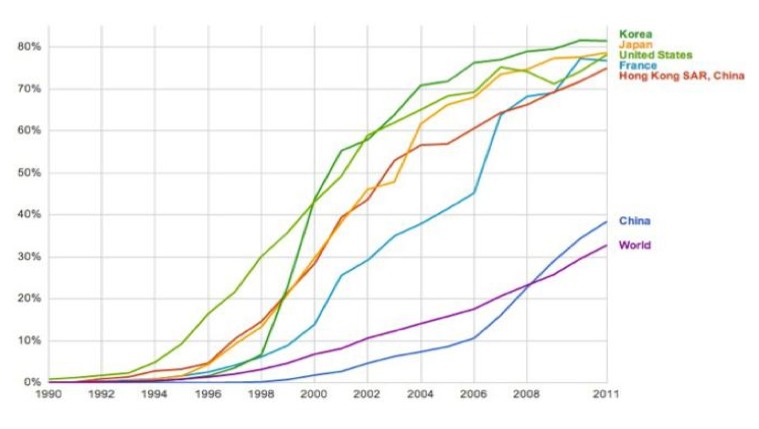
\includegraphics[width=0.7\linewidth]{imagenes/grafica-intro}
		\caption{Gráfica del crecimiento del \textit{Big Data} en algunos países y en el mundo.}
		\label{fig:grafica-intro}
	\end{figure}
	 
	 Para hacernos una idea del impacto del nacimiento de la Web 2.0, observamos la Figura \ref{fig:grafica-intro} en la que se representa el crecimiento de \textit{Big Data} en algunos países desarrollados y en el mundo en general. Notamos que en el año 1998 se produce un aumento en el ritmo de crecimiento, coincidiendo con el nacimiento de la Web 2.0. El siguiente cambio de crecimiento más brusco lo encontramos en el año 2006, año de mayor impacto de las redes sociales. 
	 
	 %Quizás nombrar en algún momento microblogging (Twitter) y esop
	 
	 Como ya veníamos advirtiendo, está en la naturaleza del ser humano dar su opinión sobre los temas que le rodean. Esta caracterización del ser humano junto con la cantidad de datos depositados por usuarios en los diferentes portales de Internet nos da una idea de la cantidad de opiniones disponibles. Esta información será de gran utilidad para las empresas que quieran conocer la opinión de los usuarios sobre un determinado producto o, simplemente, para conocer la opinión de la población sobre un determinado tema.  Sin embargo, la inmensurable cantidad de información disponible hace que contratar a personal especializado para que se dedique a estudiar las opiniones de un determinado producto o tema de actualidad sería inviable tanto desde el punto de vista económico como desde el temporal.  Debido a la necesidad de monitorizar este procedimiento surge el concepto de Análisis de Sentimientos o Minería de Opinión, del que hablaremos en los siguientes capítulos.
	 
	 Por su estructura de \textit{microblogging} (red social con un número de caracteres limitados para resaltar la opinión), Twitter es un perfecto generador de opiniones para analizar mediante Análisis de Sentimientos. Ya se han llevado a cabo estudios sobre esta plataforma obteniendo muy buenos resultados. Por ejemplo, en las últimas elecciones presidenciales de EEUU se realizó un estudio sobre la opinión de los usuarios de Twitter sobre ambos candidatos. Para este estudio se utilizaron los tweets publicados hasta 43 días antes de las elecciones comenzando el primer día de candidatura. Utilizando expertos para el etiquetado de los datos como positivos o negativos referentes a cada uno de los candidatos y entrenando con un algoritmo de Naïve Bayes consiguieron un 94\% de correlación.
	 
	 El término de Análisis de Sentimientos es un término relativamente reciente. Aunque ya haya tenido éxito en algunos ámbitos, es un campo aún sin explotar pues presenta dificultades que aún no han sido solventadas.  Entre estas dificultades se encuentran la subjetividad de las opiniones, las particularidades del lenguaje, los contextos, los sarcasmos ... entre una interminable lista.
	 
	 
	 \begin{figure}[h!]
	 	\centering
	 	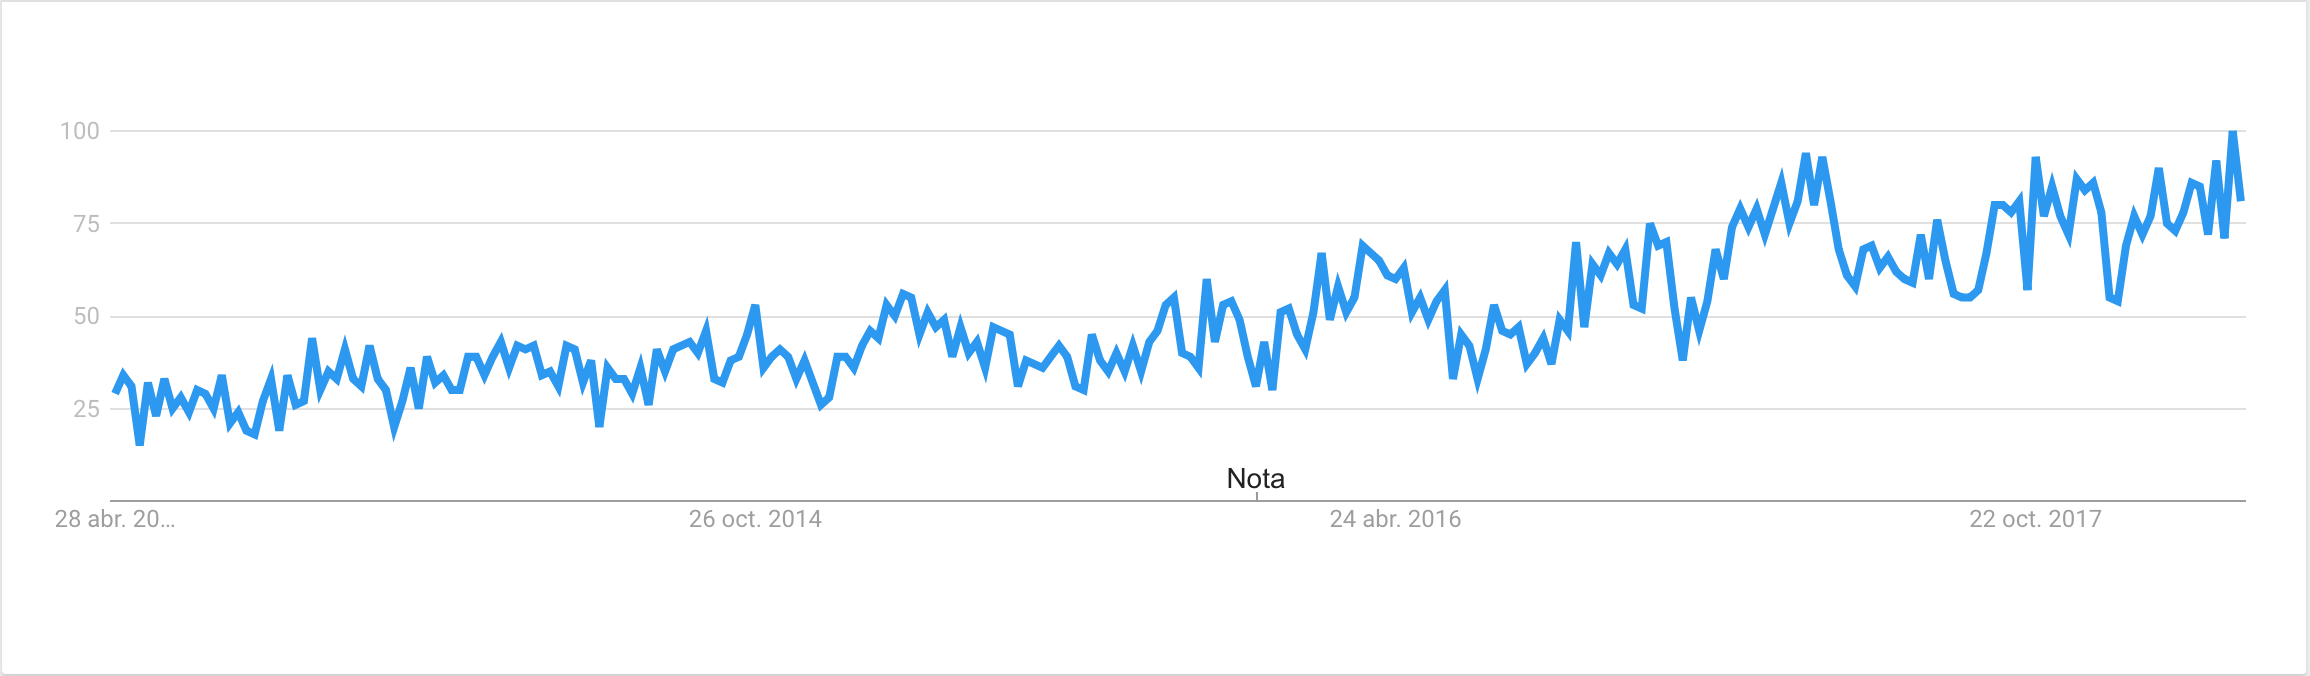
\includegraphics[width=1\linewidth]{imagenes/interes}
	 	\caption{Gráfica que representa el interés del análisis de sentimientos en todo el mundo según Google Trends.}
	 	\label{fig:interes}
	 \end{figure}
	 
	 Esto hace que se presente como una campo de estudio muy llamativo, con muchas mejoras por hacer y con un futuro muy prometedor. Cada día más gente centra su interés en esta materia (Figura \ref{fig:interes}). De ahí que a lo largo de esta memoria nos dediquemos al estudio de una parte de este amplio campo.
	 

	Como ya podemos imaginar, el término Análisis de Sentimientos abarca un gran conjunto de tareas. El trabajo se va a centrar en una de esas tareas en concreto: la extracción de características. 

	Para explicar en qué consiste y su importancia, trabajaremos sobre un ejemplo concreto. Imaginemos que queremos analizar la siguiente opinión:
	
	\begin{center}
		\begin{minipage}{0.9\linewidth}
			\vspace{5pt}%margen superior de minipage
			{\small
				[1] \textit{El ordenador tiene muy buen procesador, sin embargo la pantalla tiene poca resolución y el precio es muy elevado.}
			}
			\vspace{5pt}%margen inferior de la minipage
		\end{minipage}
	\end{center}

	Si tuviéramos que establecer una polaridad a dichar frase, sería una tarea complicada incluso para una persona. En la frase se nombran tres componentes de un mismo ordenador y se da un opinión sobre cada una de ellas. Así, \textit{buen procesador} tendría connotaciones positivas mientras que \textit{la pantalla tiene poca resolución} y \textit{el precio es muy elevado} negativas. La polaridad general del producto dependerá de la importancia que se le dé a cada una de las partes. Como no podemos saber a priori un orden de prioridad establecido, sería muy útil poder dar una polaridad a cada una de las componentes.
	
	Ahora bien, para poder realizar este proceso de forma automatizada nos encontraríamos con dos tareas: en primer lugar la identificación de la característica y, en segundo lugar, la detección de la polaridad de esta. En este trabajo nos centraremos en la primera de estas tareas. 

	\section{Objetivos} \label{objetivos}
	
	En este trabajo se pretende dar una pequeña introducción al Análisis de sentimientos, ciencia muy amplia de la que nos centraremos en resolver un tipo de problema concreto. Nuestro objetivo será resolver el problema de extracción de características.
	
	Para ponernos en contexto, realizaremos una breve introducción teórica al Análisis de sentimientos. En ella hablaremos sobre el procesamiento del Lenguaje Natural al mismo tiempo que definiremos formalmente el concepto de opinión y hablaremos de los diferentes niveles del Análisis de sentimientos donde daremos a relucir la importancia de nuestro problema concreto. 
	
	A continuación, realizaremos una introducción matemática al Deep Learning ( (?) no sé muy bien qué voy a hacer en la parte matemática) para fundamentar de forma teórica las bases de los métodos que aplicaremos en el resto del trabajo.
	
	En cuanto a la solución propuesta para resolver nuestro problema de clasificación, partiremos del modelo propuesto en el artículo de [(?) citar paper Poria]  en el que se aborda el problema con el uso de Redes Neuronales Convolutivas (CNN). Posteriormente, propondremos mejoras y/o modelos diferentes que finalmente compararemos.
	
	Así, la estructura del trabajo constaría de los siguientes tomos:
	
	 \begin{enumerate}
	 	\item Introducción teórica al Análisis de sentimientos.
	 	\item Fundamentos matemáticos del Deep Learning.
	 	\item Implementación del modelo base.
	 	\item Desarrollo de mejoras y/o nuevos modelos.
	 	\item Comparativa entre los modelos desarrollados.
	 \end{enumerate}

	 
	\section{Requerimientos}\label{requerimientos}
	
	Como ya hemos introducido en la Sección \ref{objetivos}, queremos desarrollar un software para resolver el problema de la extracción de características.
	
	Para ello, nuestro sistema aceptará un conjunto de frases con un formato determinado como entrada produciendo una secuencia de etiquetas que nos identifiquen las entidades (tanto simples como compuestas). Para ello utilizaremos el sistema de notación \textit{IOB} (IN/ OUT/ BEGING). Con este sistema, la etiqueta \textit{B} se correspondería con el inicio de una entidad. Si esta es compuesta, la siguiente palabra estaría etiquetada con la etiqueta \textit{I}. El resto de palabras que no representan una entidad serían etiquetadas con \textit{O}. 
	
	Un ejemplo de etiquetado \textit{IOB} sería el siguiente:
	
	\begin{center}
		\begin{minipage}{0.9\linewidth}
			\vspace{5pt}%margen superior de minipage
			{\small
				[1] \textit{My favourite city is New York}
				
				[2] \textit{(My, O) (favourite, O)  (city, B) (is, O) (New, B) (York, I)}
			}
			\vspace{5pt}%margen inferior de la minipage
		\end{minipage}
	\end{center}
	
	
	Para la representación de las palabras utilizaremos \textit{word embeddings} ya entrenados en diccionarios en inglés. Por lo que nuestro sistema funcionará solamente en inglés.
	

		

	



\chapter{Análisis de sentimientos}

	Para definir el concepto de Análisis de sentimientos es necesaria una breve introducción al Procesamiento del Lenguaje Natural.

\section{Procesamiento del Lenguaje Natural} \label{conceptsentiment}	
	
	 El Procesamiento del Lenguaje Natural (PLN) es un campo de la Inteligencia Artificial que se encarga de estudiar la comunicación que surge entre personas y máquinas. El objeto de estudio del PLN es, por tanto, el lenguaje. Para que las máquinas puedan conseguir capacidad de procesamiento y de generación del lenguaje, es necesario que se tenga comprensión total de la lengua. De esta misión se encarga la Lingüística, que trata de caracterizar y explicar los procedimientos del lenguaje.
	
	El procedimiento usual de un sistema PLN se divide en tres fases principales: análisis sintáctico, semántico y pragmático. En la práctica, estas fases no son suficientes. Esto se debe a que no es viable realizar el análisis sintáctico de un texto sin haber identificado las palabras y las oraciones además de la información morfológica de las palabras que componen la frase. Así, a las tres fases anteriores habría que añadir dos nuevas fases: \textit{tokenización} y análisis léxico.
	
	
	A continuación observamos el flujo de trabajo que seguiría un sistema PLN. La funcionalidad de la cada una de las fases sería:

		\begin{minipage}{.65\textwidth}
			\begin{enumerate}% never number things manually!
				\item \textit{Tokenización: }  Identificar las unidades en las que se divide el mensaje, \textit{tokens}.
				\item Análisis léxico: Obtiene información de los \textit{tokens} a partir de la función que desempeñan en la oración.
				\item Análisis sintáctico: Obtiene las relaciones y dependencias existentes entre los elementos que componen la oración.
				\item Análisis Semántico: Obtención de la intención del autor a partir de la información obtenida en la fase anterior. Busca descubrir el significado de la frase.
				\item Análisis Pragmático: Busca las conexiones entre oraciones para dar un sentido global al discurso.
			\end{enumerate}
		\end{minipage}
		\begin{minipage}{.35\textwidth}
			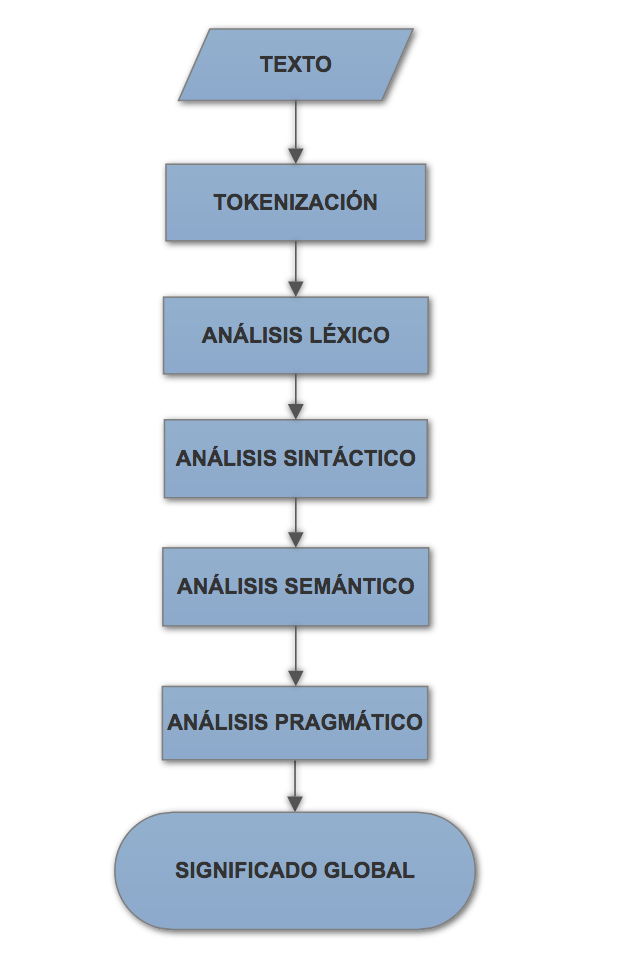
\includegraphics[width=1\linewidth]{imagenes/flujo}
		\end{minipage}
		
	La búsqueda del entendimiento del lenguaje no es la única misión del PLN. También persigue la generación automática de lenguaje, aunque no va a ser en lo que centremos esta memoria.
	
	
	
\section{Concepto de Análisis de sentimientos}\label{conceptoSA}

	El Análisis de sentimientos (AS) recibe muchos nombres dado a la evolución histórica que ha tenido: Análisis de Opiniones, Minería de Opiniones, etc. A partir de ahora y durante todo el proyecto nos referiremos a él como Análisis de sentimientos.
	
	Definimos el Análisis de sentimientos como el estudio computacional de opiniones, sentimientos y emociones expresadas en un texto. Puede ser considerado como un proceso de clasificación cuyo fin es decidir la polaridad del sentimiento expresada en el texto. La dificultad de esta ciencia recaerá en el objeto de estudio pues se trata de información desestructurada, teniendo que convertirlos en datos estructurados. 
	
	\subsection{Concepto de Opinión}\label{opinion}
	
		Como hemos comentado en la sección anterior, el objetivo del AS consite en la extracción de información a partir de textos. Fundamental para definir ese concepto será la definición de su objeto de estudio, el concepto de opinión.
		
		Una primera aproximación para la definición de opinión la encontramos en el diccionario de la RAE, una opinión es un ``juicio o valoración que se forma una persona respecto de algo o de alguien.'' De esta definición podemos destacar varias cosas. Claramente una opinión es subjetiva, juicio o valor, pero también vemos que se hace énfasis en  quién crea la opinión y sobre qué. Empezamos así a vislumbrar que la opinión estará formada por varios elementos. 
		
		Para hacer más énfasis en este concepto de opinión formada por varios elementos, veamos un ejemplo concreto:
		
			\begin{center}
			\begin{minipage}{0.9\linewidth}
				\vspace{5pt}%margen superior de minipage
				{\small
					\textit{[1] El pasado jueves fui con un grupo de amigos a cenar a un restaurante. [2] Pedí unos macarrones a la carbonara que estaban deliciosos. [3] Sin embargo, el postre no me gustó nada, pedí una tarta de queso. [4] Creo que en este sentido acertó más mi amiga María que pidió la tarta de tres chocolates, ¡le encantó! [5] En cuanto al precio, no estaba nada mal para la cantidad que servían. [6] También hay que  tener en cuenta que se encontraba a las afueras, solo se puede acceder en coche.}
				}
				\vspace{5pt}%margen inferior de la minipage
			\end{minipage}
		\end{center}
	

	Si observamos el texto anterior con la intención de extraer una opinión global sobre el restaurante, encontramos que se da información ``contradictoria'' pues hay oraciones que expresan sentimientos negativos, positivos e incluso neutros. La oración [1] expresa un hecho, sin ningún juicio de valor. Por su parte, las oraciones [2], [4] y[5] expresan sentimiento positivo mientras que las oraciones [3] y [6] expresan alguna opinión negativa. Vemos que cada una de estos juicios se realizan a ciertos elementos del restaurante, por lo que será algo a tener en cuenta dependiendo de si queremos determinar opinión de la entidad (restaurante) o de cada uno de sus componentes. Otro detalle presente en el ejemplo es que no siempre la persona que juzga algo es el autor del texto. En este caso, en la frase [4] el autor expresa que a su amiga le encantó su postre. Destacar también la importancia del tiempo a la hora de realizar un juicio de valor pues nuesta opinión puede variar a lo largo del tiempo. 
	
	En este punto, podemos considerar la opinión como una cuádrupla \textit{(o, p, h, t)} donde \textit{o} representa el objeto sobre el que recae la opinión, \textit{p} la polaridad de la misma, \textit{h} el autor y \textit{t} el tiempo en el que se produjo.
	
	Si nos fijamos en la frase [3] que expresa un sentimiento negativo, vemos que la opinión negativa no es sobre el restaurante en su conjunto si no que  es hacia un postre concreto. Según la definición de opinión como una cuádrupla \textit{(o, p, h, t)} su polaridad recaería sobre el objeto en cuestión, el restaurante. Así, surge la necesidad de considerar que el objeto pueda ser dividido en diferentes componentes. Definimos como entidad \textit{e} a un producto, servicio, tema, persona, organización o ente. Esta entidad se representa mediante \textit{(T,W)} donde \textit{T} es una jerarquía de componentes y \textit{W} el conjunto de atributos de \textit{e}. 
	
	Con esta nueva consideración llegamos a nuestra definición de opinión, introducida en \cite{liu}. Una opinión estaría formada por una quíntupla $(e_i, a_{ij}, p_{ijkl}, h_{k}, t_{l})$ donde $e_i$ representa la entidad, $a_ij$ sería el atributo de $e_i$ sobre el que recae la opinión, $p_{ijkl}$ se correspondería con la polaridad de la opinión que se hace sobre el aspecto $a_{ij}$ en el momento de tiempo $t_{l}$ por la persona $h_{k}$ y, por último, $h_{k}$ y $t_{l}$ la persona y el tiempo en que se realiza el juicio de valor respectivamente.
		 
		
	\subsection{Niveles de clasificación}\label{nivelesSA}
	
	%Aqui hacer mucho énfasis en lo importante que es hacerlo por entidades -> Dar importancia a mi trabajo
	
	Como ya hemos introducido, el objetivo final del Análisis de sentimientos es la clasificación de un texto según su polaridad. Ahora bien, a la hora de clasificar la polaridad de un texto podemos considerar tres niveles:
	
	\begin{enumerate}
		\item \textbf{Nivel de texto: } Analiza el documento completo y asigna una polaridad global al documento en su conjunto. Es el nivel más general y, por tanto, menos preciso.
		\item \textbf{Nivel de sentencias: } Detecta el sentimiento en frases. Está muy relacionado con la subjetividad ya que esta se expresa en frases y no en documentos largos. Obtendríamos uan clasificación más precisa del sentimiento.
		\item \textbf{Nivel de aspectos o entidades: } Detecta el sentimiento u opinión y la entidad a la que se refiere. Es el nivel más preciso de análisis, pues no produce generalizaciones si no que se identifica una polaridad con un aspecto concreto.
	\end{enumerate}
	
	 Como ya hemos comentado, nuestro proyecto se centrará en el último de estos niveles de clasificación. La importancia de esta especificación queda reflejada en el ejemplo que pusimos en la sección \ref{opinion}. Además, una vez tengamos clasificada la polaridad de los diferentes aspectos o entidades, es fácilmente extrapolable al resto de niveles de clasificación. Podemos obtener la clasificación a nivel de sentencias simplemente con la combinación de la polaridad de cada uno de los aspectos que aparecen en la sentencia y análogamente con la clasificación a nivel de texto.
%\chapter{Metaheurísticas y computación evolutiva}
En este capítulo haremos un repaso teórico sobre qué son las metaheurísticas en la Sección \ref{meta} y más concretamente qué es la programación evolutiva (Sección \ref{evolution}), ya que emplearemos estos para la optimización de forma conjunta de las herramientas de análisis de sentimientos, mediante la búsqueda de pesos que se le darán a las herramientas con el fin de reducir la tasa de error con respecto al etiquetado experto.

\section{Concepto de metaheurística} \label{meta}
En esta sección hablaremos de qué es una metaheurística y en qué casos se suelen usar (Sección \ref{conceptmeta}), así como qué componentes de una metaheurística hay que tener en cuenta a la hora de diseñarlas y desarrollarlas (Sección \ref{componentesmeta})

\subsection{¿Qué son las metaheurísticas?} \label{conceptmeta}
Para explicar qué es una metaheurística primero habría que analizar la morfología de la propia palabra. En la Inteligencia Artificial, el término \textit{heurística}, como podemos ver en \cite{meta}, se refiere a una técnica, método o procedimiento inteligente de realizar una tarea que no es producto de un riguroso análisis formal, sino de conocimiento experto sobre la tarea.  En especial, se usa el término heurístico para referirse a un procedimiento que trata de aportar soluciones a un problema con un buen rendimiento, en lo referente a la calidad de las soluciones y a los recursos empleados. Al término 'heurística' se le une el sufijo \textit{meta}, que significa 'más allá' o 'a un nivel superior'. Las \textit{metaheurísticas} son estrategias inteligentes para diseñar o mejorar procedimientos heurísticos muy generales con un alto rendimiento.

Existen muchísimos problemas cuya complejidad puede suponer que un algoritmo voraz no nos pueda dar una solución o que nos la pueda dar en tiempos inadmisibles. Un claro ejemplo es el problema del Viajante de comercio (\textit{Travelling Salesman Problem o TSP}), que consiste en que, con un número de ciudades concreto y las distancias entre cada una de ellas, realizar la ruta más óptima tal que salgamos de una ciudad, pasemos por todas y, finalmente, lleguemos a la misma ciudad. Este problema es un problema NP-duro, y a partir de un número de ciudades determinado, una solución mediante algoritmos voraces puede suponer tiempos de ejecución de incluso años.

La solución a estos problemas puede ser imposible de obtener. Una metaheurística es un algoritmo aproximado que pretende ofrecernos una solución óptima o de calidad aceptable a un problema. Su funcionamiento se basa en la minimización o maximización de una función objetivo, que evaluará la calidad de las soluciones, empleando para ello diferentes técnicas como la aletoriedad o, como en la programación evolutiva, 'fusión' entre soluciones de calidad.

Existen varias maneras de clasificar una metaheurística. Una de las clasificaciones más empleadas distingue entre los 3 siguientes tipos de metaheurísticas:
\begin{itemize}
	\item \textbf{Metaheurísticas basadas en métodos constructivos. }Se caracterizan por construir una solución definiendo diferentes partes de ella en sucesivos pasos.
	\item \textbf{Metaheurísticas basadas en trayectorias. }Son metaheurísticas en las que la heurística subordinada es un algoritmo de búsqueda local que sigue una trayectoria en el espacio de búsqueda.
	\item \textbf{Metaheurísticas basadas en poblaciones. }En estas metaheurísticas un conjunto de soluciones se combinan para obtener nuevas soluciones que heredan algunas propiedades de las primeras. Dentro de este tipo se encuentran las metaheurísticas basadas en computación evolutiva, que son las que se emplearán en este proyecto.
\end{itemize}
\subsection{Componentes de las metaheurísticas} \label{componentesmeta}
Para la implementación de una metaheurística es necesario tener claras cuáles son las componentes de estas y qué aspectos son necesarios para tenerlos en cuenta para así tener soluciones de la máxima calidad posible. Estas componentes y aspectos son los siguientes:
\begin{itemize}
	\item \textbf{Esquema de representación. }Se trata de la forma de representar la solución a un problema. Cada problema y metaheurística tiene una representación más o menos adecuada. Por ejemplo, en TSP \footnote{\textit{Travelling Salesman Problem} anteriormente comentado} una buena representación de la solución es una permutación de  $ \{1,...,n\} $ indicando el orden de 'visita' de cada ciudad. Poniendo otro ejemplo, en un problema de selección de características para aprendizaje automático, podría representarse como un array de booleanos.
	\item \textbf{Función objetivo. }Se trata de la función que hay que optimizar. Esta función debe dar una valoración de una solución determinada. Por ejemplo para el TSP habría que calcular la distancia recorrida siguiendo el orden dado por la representación de la solución.
	\item \textbf{Movimiento. }Se trata de la operación que transforma una solución en otra, normalmente tratándose esta de una solución vecina. Por ejemplo, en el TSP una posible transformación podría ser intercambiar el orden de visita de 2 ciudades.
	\item \textbf{Exploración y explotación. }Son 2 aspectos muy importantes a la hora de la implementación. La exploración se refiere a la habilidad de nuestro algoritmo de explorar en distintos espacios de búsqueda o, menos formalmente, introduce más aleatoriedad a la generación de nuevas soluciones. La explotación, sin embargo, consiste en explotar espacios de búsqueda prometedores, es decir, a partir de una solución de calidad, analizar soluciones 'cercanas' a esta. Una buena metaheurística intenta mantener un equilibrio entre la exploración y la explotación.
\end{itemize}

\section{Computación evolutiva} \label{evolution}
En esta sección se introducirá a lo que es la computación evolutiva. En la Sección \ref{conceptevo} se hablará del concepto de computación evolutiva. En la Sección \ref{componentesevo} mencionaremos las principales componentes de un algoritmo evolutivo.

\subsection{Concepto de computación evolutiva} \label{conceptevo}
La computación evolutiva (\cite{evolution} y \cite{evolution2}) está compuesta por modelos de evolución basados en poblaciones cuyos elementos representan soluciones a problemas. Se trata de un conjunto de técnicas de optimización probabilística que se pueden clasificar como metaheurísticas basadas en poblaciones.

La computación evolutiva basa su funcionamiento en un proceso tan básico en la naturaleza como la evolución natural. Algunas de las características que la computación evolutiva hereda de la evolución natural son:
\begin{itemize}
	\item Capacidad de un individuo o entidad de reproducirse.
	\item Existe variedad y diversidad dentro de la población.
	\item La variedad está directamente asociada con la habilidad para sobrevivir en el entorno, es decir, con la adaptación del individuo al entorno.
\end{itemize}

En la figura \ref{geneticos} se puede observar la relación entre las computación evolutiva y la evolución natural.

\newpage

\begin{figure} [H]
	\centering
	\includegraphics[width=0.7\linewidth]{imagenes/geneticos}
	\caption{Relación metafórica entre la computación evolutiva y la evolución natural. Fuente: SCI2S UGR asignatura Metaheurísticas}
	\label{geneticos}
\end{figure}
%TODO poner aquí las secciones

\subsection{Componentes y proceso de un algoritmo evolutivo}\label{componentesevo}
A la hora del desarrollo de un algoritmo evolutivo, es necesario conocer las componentes de estos y el proceso que estos suelen seguir. Las componentes indispensables en un algoritmo evolutivo son las siguientes:
\begin{itemize}
	\item \textbf{Una población} formada por individuos o cromosomas, que serán realmente un conjunto de soluciones.
	\item \textbf{Un criterio de selección} que determinará qué individuos de la población actual sobrevivirán y seguirán en la siguiente generación de individuos. Este criterio de selección simula la selección natural dentro de la evolución.
	\item \textbf{Un operador de cruce} que cree una nueva solución a partir de la recombinación de otras. A la hora del cruce hay que tener en cuenta otros aspectos como por ejemplo la probabilidad de cruce, el criterio con el que se eligen los padres o el cómo se realizará el cruce. Este operador simula la reproducción en los seres vivos.
	\item \textbf{Operador de mutación} cuyo fin es introducir diversidad en la población. Hay que planificar de qué manera se realizará la mutación y con qué probabilidad se mutará.
	\item \textbf{Criterio de parada} que será cuando nuestro algoritmo termine su ejecución. El criterio frecuentemente se trata de un número máximo de evaluaciones de la función objetivo o también de un límite de tiempo. 
\end{itemize}

El procedimiento de un algoritmo evolutivo puede verse representado en la figura \ref{fig:geneticosproceso}. Partimos de una población o conjunto de soluciones, normalmente generada de forma aleatoria. A partir de esta población, hacemos una selección de individuos siguiendo algún criterio determinado, como el torneo binario que posteriormente comentaremos. Después, se realizará el cruce entre individuos, siguiendo criterios determinados para seleccionar los padres y para el propio cruce. Por último, se realizan mutaciones sobre la población resultante con una determinada probabilidad de que ocurra

\begin{figure} [H]
	\centering
	\includegraphics[width=0.7\linewidth]{imagenes/geneticosproceso}
	\caption{Orden del proceso en un algoritmo evolutivo. Fuente: SCI2S UGR asignatura Metaheurísticas}
	\label{fig:geneticosproceso}
\end{figure}




%\chapter{Preparación de los experimentos} \label{preparacionexperimentos}
%TODO poner aquí las secciones
%TODO avisar también de qué he hecho en R, qué en C++, etc.
En este capítulo se explicará el procedimiento para la realización de los experimentos. En la Sección \ref{toolsanalysis} se hablará de las herramientas, de cómo se han realizado los experimentos con estas y qué aspectos se han tenido en cuenta, así como de los \textit{datasets} empleados para la experimentación. Posteriormente se explicará el proceso completo para la búsqueda de pesos con el fin de optimizar las tasas e error en los distintos conjuntos de datos (Sección \ref{evolutionpreparation}).

%TODO Métricas
\section{Análisis de las herramientas} \label{toolsanalysis}
En esta sección se presentará un resumen de los conjuntos de datos empleados (Sección \ref{datasets}) para la experimentación y hablaremos de cada herramienta individualmente más en detalle y cómo se han realizado los experimentos con cada una de estas en la Sección \ref{toolsdescription}. Posteriormente, en la Sección \ref{ensamble} se explicarán las dos estrategias de ensamblado usadas y finalmente, en la Sección \ref{metricas} se explicarán las métricas que se emplearán para la comparación de herramientas.

\subsection{Conjuntos de datos} \label{datasets}
Los conjuntos de datos han sido proporcionados por Matheus Araújo y su equipo de investigación. Son los mismos conjuntos de datos con los que ellos realizaron su estudio en \cite{rib}. Se tratan de 18 conjuntos de datos tomados de distintas fuentes, como podemos ver en la tabla \ref{tabla_datos}. El etiquetado de los comentarios ha sido realizado por humanos, Amazon Mechanical Turk \footnote{https://www.mturk.com/mturk/welcome} (AMT) o, como en los casos de comentarios valorando películas, mediante la valoración dada por el usuario a la propia película. Todos los conjuntos de comentarios están etiquetados como \textit{positive}, \textit{negative} y \textit{neutral}, aunque algunos no contienen comentarios con esta última etiqueta.

%TODO explicar los conjuntos de datos individualmente
Entre los conjuntos de datos se ve diversidad en los contextos en los que los comentarios se realizan. Hay tweets en contextos concretos (como los de debate político), tweets cogidos aleatoriamente, valoraciones de películas, comentarios en vídeos de YouTube o evaluaciones sobre productos en Amazon. Hay otros conjuntos de comentarios que son en contextos concretos, como por ejemplo sentistrength\_bbc, vader\_nyt y sentistrength\_digg que son comentarios de gente en determinados foros de discusión sobre noticias en el diario BBC, \textit{New York Times} y la revista Digg. Al tratarse de hilos de comentarios, estos comentarios dependen de los anteriores, por lo que aunque sean sobre dominios concretos, la polaridad podría depender de otros comentarios, dificultando la extracción de polaridad incluso por la parte del experto. 


En la Tabla \ref{tabla_datos}, además, también se puede observar el número de comentarios de cada conjunto, cuántos son positivos, negativos o neutros, la media de frases por comentario, la media de palabras por comentario y también cómo nos referiremos a estos conjuntos de datos en el proyecto (nombre de los ficheros de datos).

\newpage
	\begin{table}[H] 
		\small
		\scalebox{0.7}{
	\begin{tabular}{|b{1.8cm}b{1.3cm}b{1.3cm}b{1.3cm}b{1.3cm}b{1.5cm}b{1.9cm}c|}
		\hline		
		\rowcolor{lightgray} 
		\textbf{Dataset} &  \textbf{Msg} & \textbf{Pos} & \textbf{Neg} & \textbf{Neu} & \textbf{Media frases} & \textbf{Media palabras} & \textbf{Nombre fichero} \\ 
		\hline  
		Comments (BBC)& 1000 & 99 & 653 & 248 & 3.9 & 64.39  & sentistrength\_bbc  \\ 
		\hline 
		Comments (Digg) & 1077 & 210 & 572 & 295 & 2.5 & 33.97 & sentistrength\_digg \\ 
		\hline 
		Comments (NYT) & 5190 & 2204 & 2742 & 274 & 1.01 & 17.76 & vader\_nyt \\ 
		\hline 
		Comments (TED) & 839 & 318 & 409 & 112 & 1 & 16.95 & nikolaos\_ted \\ 
		\hline 
		Comments (Youtube)& 3407 & 1665 & 767 & 975 & 1.78 & 17.68  & sentistrength\_youtube  \\ 
		\hline 
		\specialcell{Movie\\reviews} & 10662 & 5331 & 5331 & - & 1.15 & 18.99  & pang\_movie    \\ 
		\hline 
		\specialcell{Movie\\reviews} & 10605 & 5242 & 5326 & 37 & 1.12 & 19.33   & vader\_movie   \\ 
		\hline 
		Myspace posts & 1041 & 702 & 132 & 207 & 2.22 & 21.12  & sentistrength\_myspace  \\ 
		\hline 
		Product Reviews (Amazon) & 3708 & 2128 & 1482 & 98 & 1.03 & 16.59  & vader\_amazon   \\ 
		\hline 
		Tweets (Debate)& 3238 & 730 & 1249 & 1259 & 1.86 & 14.86 & debate  \\ 
		\hline 
		Tweets (Random)& 4242  & 1340 & 949 & 1953 & 1.77 & 15.81  & sentistrength\_twitter   \\ 
		\hline 
		Tweets (Random)& 4200 & 2897 & 1299 & 4 & 1.87 & 14.10  & vader\_twitter  \\ 
		\hline 
		Tweets (Random)& 3771 & 739 & 488 & 2536 & 1.54 & 14.32  & english\_dailabor  \\ 
		\hline 
		Tweets (Random)& 500 & 139 & 119 & 222 & 1.90 & 15.44 & aisopos\_ntua    \\ 
		\hline 
		\specialcell{Tweets\\(Specific\\Domains)}& 359 & 182 & 177 & - & 1.0 & 15.1  & stanford\_tweets   \\ 
		\hline 
		\specialcell{Tweets\\(Specific\\Topics)}& 3424  & 580 & 654 & 2503 & 1.6 & 15.03  & sanders   \\ 
		\hline 
		\specialcell{Tweets\\(SemEval\\2013)}& 6087 & 2223 & 837 & 3027 & 1.86 & 20.05  & tweet\_semevaltest    \\ 
		\hline 
		\specialcell{Runners\\World\\Forum}& 1046 & 484 & 221 & 341 & 4.79 & 66.12  & sentistrength\_rw   \\ 
		\hline 
	\end{tabular}
}
	\caption{Tabla resumen de los \textit{datasets} usados para la experimentación}
	\label{tabla_datos}
\end{table}

\subsection{Métodos de análisis de sentimientos} \label{toolsdescription}
En esta subsección se describirá cada herramienta de extracción de polaridad y cómo se han realizado los experimentos con estas. Además, cada herramienta nos da una salida distinta, por lo que se tienen que normalizar las salidas con el fin de realizar una comparativa entre ellas y posteriormente analizar su comportamiento de forma ensamblada. Las salidas han sido normalizadas en el intervalo [0,1] y para analizar sus tasas de acierto con respecto al etiquetado experto, se han aplicado las etiquetas de la siguiente manera según la intensidad de la polaridad, siendo $x$ la intensidad:
\begin{itemize}
	\item \textbf{Negativa} si $0 \leq x \leq 0.33$
	\item \textbf{Neutra} si $0.33 < x \leq 0.66$
	\item \textbf{Positiva} si $0.66 < x \leq 1$
\end{itemize}

\subsubsection{CoreNLP}
 \textbf{\textit{Standford} CoreNLP} \cite{corenlppaper} es un software desarrollado por la Universidad de Standford que ofrece un paquete de herramientas de análisis de lenguaje natural, como por ejemplo la categorización gramatical de las palabras o la obtención del sentimiento que una frase transmite. Además, ofrece funcionalidad para varios idiomas, aunque para algunas herramientas, como la de análisis de sentimientos, solo admiten el inglés.
 
 La herramienta de análisis de sentimientos se basa en un modelo de aprendizaje automático, más concretamente una red neuronal, como se puede leer en \cite{corenlpfuncionamiento}. Para obtener este modelo han usado un conjunto de datos de comentarios sobre películas los cuales han separado en frases y han obtenido el etiquetado experto de cada frase empleando AMT.
 
 CoreNLP es una herramienta que nos da la polaridad a nivel de frase. Además nos ofrece una salida categórica, donde las etiquetas son \textit{very negative, negative, neutral, positive} y \textit{very positive}. Para obtener el sentimiento numérico total del comentario, averiguo el sentimiento medio haciendo la media de las polaridades de cada frase del comentario. La normalización de la salida se ha realizado asignando los siguientes valores a cada una de las etiquetas para cada frase:
 \begin{itemize}
 	\item 0 si la etiqueta es \textit{very negative}.
 	\item 0.25 si la etiqueta es \textit{negative}.
 	\item 0.5 si la etiqueta es \textit{neutral}.
 	\item 0.75 si la etiqueta es \textit{positive}.
 	\item 1 si la etiqueta es \textit{very positive}.
 \end{itemize}

Para usar CoreNLP se ha usado la librería coreNLP de R. Siguiendo las instrucciones de la documentación dentro del GitHub \cite{corenlpgithub} de esta librería, he implementado la siguiente función en R, que será aplicada sobre cada uno de los conjuntos de datos.

\begin{lstlisting} [language = R]
 obtenerSentimiento <- function(datos)
 {
  comments.datos <- lapply(datos, c)
  comments.datos <- lapply(comments.datos, annotateString)
  sentiments.datos <- lapply(comments.datos, getSentiment)
  label.datos <- sapply(sentiments.datos, assign.polarity)
  return(unlist(label.datos))
 }
\end{lstlisting}

Donde la función assign\_polarity será la que asigne la polaridad media a cada comentario.

%TODO poner aquí las funciones en R así como la de asignación de etiqueta, mejorar el código

\subsubsection{Azure Text Analytics}
Se trata de una API de Microsoft Azure con fines comerciales pero que aún así ofrece una versión de prueba gratuita con hasta 5000 llamadas de la función para obtener el sentimiento. Además de análisis de sentimiento, este software tiene otras herramientas tales como la detección de \textit{topics} o temas o detección de idiomas. Al tratarse de una herramienta comercial, no hay gran información sobre cómo se implementa la clasificación de los comentarios, aunque en su documentación \cite{azuredoc} se menciona que usa técnicas de clasificación, tomando como características de entrada '\textit{n-grams}' de palabras (que son conjuntos de $n$ palabras) y características generadas mediante técnicas de \textbf{\textit{POS}}  y \textbf{\textit{Stemming}}. La salida de la herramienta de análisis de sentimiento nos devuelve un valor en [0,1], por lo que no ha tenido que ser normalizada, indicando un sentimiento cercano a 1 un sentimiento positivo y cercano a 0 un sentimiento negativo.

Para utilizar esta API se ha usado la biblioteca mscstexta4r para R. Antes es necesario crear una cuenta en los servicios de \textit{Machine Learning} de Microsoft, donde obtendremos una clave que debemos declarar como variable de entorno del sistema. Después solo hay que inicializar el entorno con la función textaInit y ya ejecutar la función textaSentiment introduciéndole como argumentos el conjunto de datos en forma de Array y un Array con el idioma de los comentarios repetidos tantas veces como comentarios haya en nuestro fichero. La función textaSentiment acepta en una ejecución un máximo de 500 comentarios por lo que hay que realizar división de algunos conjuntos de datos.

\subsubsection{MeaningCloud}
MeaningCloud \cite{meaningclouddoc} es también una herramienta con fines comerciales. Nos ofrece unas 40.000 consultas de polaridad mensualmente en la tarifa gratuita, aunque también ofrece licencias especiales para estudiantes. Su funcionamiento se basa tanto en el análisis morfo-sintáctico de los textos así como en la utilización del significado de las palabras (diccionarios) para identificar intensidades. Además, esta herramienta es muy flexible ya que nos permite crear nuestros propios diccionarios para la extracción de información de los textos, nuestros propios modelos de clasificación de textos, e incluso nuestros propios modelos de sentimiento para adaptar el análisis de polaridad a nuestro dominio, añadiendo conjuntos de comentarios con su etiquetado para el aprendizaje.

La salida de este software, la cual es a nivel de documento, nos devuelve 6 valores discretos, aunque uno de ellos, \textit{NONE}, indica que el comentario no emite ningún sentimiento, por lo que \textit{NONE} lo consideramos como neutral. Así, se nos quedan 5 valores discretos igual que en CoreNLP, por lo que el paso a valor numérico y normalización en [0,1] es la misma que para CoreNLP.

Para realizar los experimentos primero tenemos que crear una cuenta en MeaningCloud y obtener una clave para la utilización de los servicios del software. Después, en R, generamos una url (https://api.meaningcloud.com/sentiment-2.1?key= $<$ clave $>$ \&of=json\&txt= $<$ comentario $>$ \&lang=en) y mediante una petición POST con la librería \textit{httr} recibimos un JSON, del que solo necesitamos el elemento \textit{score\_tag}.

\subsubsection{SentiStrength}
Este software es también una herramienta de análisis de sentimiento con fin comercial pero con una versión java gratuita para investigación académica. SentiStrength (\cite{senti} y \cite{senti2}) es una herramienta que se basa en un diccionario de palabras que expresan sentimiento con un valor asociado que mide la intensidad de ese sentimiento, empleando además aprendizaje automático para optimizar este diccionario e información lingüística y reglas adicionales.

SentiStrength nos da la salida a nivel de documento y devuelve 2 valores de salida: uno que nos dice cómo de positivo es el comentario y otro que nos dice cómo de negativo es. Para el valor positivo nos devuelve valores discretos y enteros en [1,5], indicando 1 que el comentario no expresa nada de sentimiento positivo y 5 que expresa un sentimiento muy positivo; para el valor negativo la salida es igual a excepción de que esta son valores negativos.

Este software ha sido el más fácil de usar, ya que gracias a la versión java gratuita para investigación en educación (amablemente facilitada por Mike Thelwall, así como sus diccionarios más actualizados), lo único que hay que hacer es ejecutarla introduciéndole como argumentos el fichero de comentarios y los datos o diccionarios.

Para normalizar la salida y equipararla a la de las demás, lo que se ha realizado en este proyecto es obtener la suma de la polaridad positiva y la negativa. Así, el valor negativo indica un sentimiento negativo y el valor positivo un sentimiento positivo. Si es 0, es un sentimiento neutro. Para normalizar esto en [0,1], tenemos que asegurarnos de que un valor negativo esté en el intervalo [0,0.33] y que un valor positivo esté en el intervalo (0.66,1]. Para ello se emplea la siguiente fórmula:

Siendo:
\begin{itemize}
	\item $[a,b]$ el intervalo en el que quiero normalizar.
	\item $[min, max]$ el intervalo en el que se encuentra la salida (positiva o negativa). Por ejemplo, para la positiva $min$ sería 1 y $max$ sería 4.
	\item $x$ el valor de la intensidad de la actual instancia o comentario.
	\item $f(x)$ el nuevo valor de la polaridad ya normalizado.
\end{itemize}

Entonces:
$$ f(x) = [ (b-a)(x-min) / (max - min) ] + a$$

\subsubsection{VADER}
VADER \cite{vader} (\textit{Valence Aware Dictionary and sEntiment Reasoner}) es un SAM basado en diccionario y en reglas que está especialmente ajustado para funcionar bien con textos de los medios de comunicación y \textit{tweets}. Su salida, a nivel de documento, es devuelta en el intervalo [-1,1] siendo 1 lo más positivo posible y -1 lo más negativo posible. Debemos coger de su salida el componente '\textit{compound}', que contiene la valoración global del comentario. La normalización se puede realizar mediante una normalización min-max normal, ya que en este caso no hay que tener en cuenta aspectos como en SentiStrength, Bing o Syuzhet.

Para realizar los experimentos con este software, hay que instalar primero python y el software de VADER, siguiendo las instrucciones de la documentación. Posteriormente, he tomado como referencia un código aportado por Matheus Araújo y disponible en el repositorio \footnote{https://bitbucket.org/matheusaraujo/sentimental-analysis-methods} del equipo de investigación. Para ejecutarlo solo he tenido que ejecutar mediante python el ficher vader.py con el argumento -f $<$fichero$>$.

\subsubsection{Bing y Syuzhet}
Aunque se tratan de dos SAM distintos \cite{syuzhet}, los describiré juntos ya que ambos han sido utilizados mediante la misma biblioteca de R. Ambos SAM son basados en diccionarios. Bing es un diccionario desarrollado por Minqing Hu y Bing Liu, mientras que el diccionario syuzhet fue desarrollado en \textit{Nebraska Literary Lab} bajo la dirección de Matthew L. Jockers.

La salida de ambas herramientas es a nivel de frase, por lo que para obtener la polaridad global del comentario se ha realizado haciendo una media aritmética de las polaridades de cada frase. Los 2 SAMs devuelven valores que no tienen por qué estar en un intervalo concreto, pero los autores afirman que si la salida es negativa entonces el sentimiento es negativo y si es positiva es positivo. Por lo tanto la salida de los comentarios han sido normalizadas con una normalización min-max en la que además hay que tener en cuenta los aspectos tenidos en cuenta con SentiStrength, donde todo valor negativo debe encontrarse en [0,0.33] y todo valor positivo en (0.66,1].

Para ejecutar ambas herramientas he usado el paquete syuzhet para R. La función para obtener el sentimiento es muy parecida a la de coreNLP:
\begin{lstlisting} [language = R]
obtenerSentimiento <- function(datos)
{
 comments.datos <- lapply(datos, c)
 comments.datos <- lapply(comments.datos, get.sentences)
 sentiments.datos <- lapply(comments.datos, get.sentiment,
    method="method")
 label.datos <- sapply(sentiments.datos, assign.polarity)
 return(unlist(label.datos))
}
\end{lstlisting}

Donde la función assign\_polarity será la que asigne la polaridad media a cada comentario y method será 'bing' o 'syuzhet' dependiendo del método que se vaya a emplear.

\subsection{Análisis del ensamblado de las herramientas} \label{ensamble}
Como preámbulo de la optimización mediante asignación de pesos del funcionamiento conjunto de las herramientas, se va a realizar un análisis de cómo estas herramientas funcionan de forma ensamblada. Se realizarán dos modelos distintos, descritos a continuación:
\begin{itemize}
	\item \textbf{Sentimiento promedio.} Es el modelo más intuitivo y consiste en asignar la polaridad media teniendo en cuenta la polaridad devuelta por todas las herramientas. De esta manera, la polaridad $P(X)$ se describe como se expresa a continuación:
	$$P(x) = \frac{1}{N}\sum_{i=1}^{N}p_i$$
	Donde $p_i$ es la polaridad devuelta por la herramienta $i$ y $N$ el número de herramientas.
	\item \textbf{Ensamblado proneutral.} Basándonos en el estudio en \cite{proneu}, donde este operador obtiene los mejores resultados del estudio, se empleará este operador con el fin de dar más peso a las herramientas que ofrece una polaridad más neutra. Para el cálculo de pesos para cada instancia, primero se obtienen unos $e_i$ que vienen definidos por $e_i = 1-|p_i-0.5|$ donde $p_i$ es la polaridad dada por por la herramienta $i$ para esa instancia. A partir de estos $e_i$ se obtienen los pesos $w_i$ mediante la expresión: 
	$$w_i=\frac{e_i}{\sum_{j=1}^{N}e_j}$$ donde $N$ es el número de herramientas. A partir de estos pesos se obtiene el sentimiento global del comentario:
	$$P(x)=\sum_{i=1}^{N}w_ip_i$$
\end{itemize}

\subsection{Medidas empleadas para el análisis}  \label{metricas}
Para la comparación de las distintas herramientas emplearemos varias medidas que indican la calidad de la predicción. Estas medidas son las siguientes:
\begin{itemize}
	\item \textbf{Error de clasificación.} Se trata del cociente del número de instancias mal clasificadas entre el número total de instancias. Es una de las medidas más importantes en nuestro análisis y la más intuitiva.
	\item \textbf{Área bajo la curva (\textit{Area Under Curve o AUC}).} El área bajo la curva se puede interpretar como la probabilidad de que un clasificador puntúe una instancia positiva elegida aleatoriamente más alta que una negativa, es decir, que el clasificador la considere 'más positiva' que la negativa. El AUC solo se puede calcular en problemas de clasificación con 2 clases. Al tratarse este un problema de 3 clases, calcularemos la AUC siguiendo una estrategia \textit{one vs all} que consiste en considerar una clase como positiva y el resto como negativas y calcular el AUC, realizando esto para cada clase. El AUC final sería la media de las AUCs. Para calcular el AUC multiclase empleo la función multiclass.roc de la librería pROC, que ya implementa la estrategia explicada.
	\item \textbf{\textit{Recall.}} El \textit{recall} se trata del cociente del número de instancias de una clase acertadas entre el número total de elementos de esa clase o, más formalmente, $Recall = \frac{tp}{tp+fn}$ donde $tp$ (True Positive) es el número de instancias positivas bien clasificadas y $fn$ (False Negative) es el número de instancias predichas como negativas pero en realidad son positivas.
	\item \textbf{Precisión.} La precisión es el cociente entre el número de instancias de una clase correctamente clasificadas entre el número total de instancias que se han clasificado con esa clase. Formalmente se define como $Precision = \frac{tp}{tp+fp}$ donde $fp$ son las instancias clasificadas como positivas pero que en realidad son negativas.
\end{itemize}

Estas últimas medidas (\textit{recall} y precisión) se han usado con el fin de contrastar y matizar más los resultados que se obtienen con las AUCs.

\begin{figure} [H]
	\centering
	\includegraphics[width=0.4\linewidth]{imagenes/precisionrecall}
	\caption{Explicación gráfica de qué son el Recall y la precisión. Fuente: Wikipedia}
	\label{fig:precisionrecall}
\end{figure}


\section{Optimización mediante algoritmos evolutivos} \label{evolutionpreparation}
En esta sección se describirá primero el procedimiento general para la optimización (Sección \ref{preparacionevo}), tanto la preparación de los ficheros de datos como el tipo de validación que se empleará. También se describirán los algoritmos (Sección \ref{algorithms}) evolutivos que se emplearán, describiendo detalladamente tanto sus componentes como su pseudocódigo. Finalmente, como se desarrollará software para la ejecución de los algoritmos, en la Seccion \ref{is} se realizará una sección para detallar un poco más las funciones auxiliares a los algoritmos y la utilización del programa.
\subsection{Preparación de datos y validación} \label{preparacionevo}
La ejecución de las metaheurísticas se realizará sobre los resultados continuos que hemos obtenido de la ejecución de las herramientas. Para ello, mediante un script en R, crearemos un fichero de datos para cada conjunto de datos, cuyas filas representarán cada comentario, teniendo estos 7 características que serán las polaridades de cada herramienta para este comentario y un valor 'etiqueta' que será el sentimiento experto del comentario.

Nuestro algoritmo nos dará una combinación lineal del producto de los pesos buscados por el algoritmo y la intensidad de cada herramienta, tal y como se describe a continuación:
$$P(x) = \sum_{i=1}^{n}w_i*p_i$$
donde:
\begin{itemize}
	\item $P(x)$ es la polaridad final del comentario $x$.
	\item $n$ es el número de características, en nuestro caso 7 (una por cada herramienta).
	\item $w_i$ es el peso que nuestro algoritmo asigna a la herramienta $i$, normalizados en $[0,1]$ y tal que la suma de todos los $w_i$ sumen 1.
	\item $p_i$ es el valor de la polaridad de la herramienta $i$ en el comentario $x$.
\end{itemize}

 Todos los algoritmos tendrán en común la función objetivo, es decir, la función que hay que optimizar. La función objetivo es el error cuadrático medio, el cual tendremos que reducir. Este error lo calcularemos con respecto al etiquetado del conjunto de datos de train, es decir, un 80\% de los comentarios (el otro 20\% se empleará posteriormente para la validación). El error cuadrático medio viene definido por la siguiente expresión, siendo $Y'$ un vector de $n$ predicciones e $Y$ un vector que contiene los verdaderos valores:
 $$ECM = \frac{1}{n}\sum_{i=1}^{n}(Y'_i-Y_i)^2$$
 
 La validación para el aprendizaje de los pesos se realizará mediante una validación cruzada \textit{5-fold cross validation}, que consiste en dividir el conjunto de datos en 5 subconjuntos realizando 5 iteraciones donde en cada iteración aprenderemos con 4 subconjuntos y validaremos con uno. Para realizar la valoración de los resultados emplearemos un error de clasificación normal, para así poder dar una mejor interpretación.
 
 Otro aspecto en común de todos los algoritmos es el criterio de parada. Todos los algoritmos evolutivos tendrán como criterio de parada la evaluación de un máximo de 500.000 veces la función objetivo.
 
 \subsection{Descripción de los algoritmos} \label{algorithms}
 En esta sección se describirá cada uno de los algoritmos evolutivos que se emplearán para la optimización. Se describirán tanto las componentes del algoritmo como su funcionamiento y pseudocódigo.
 
 \subsubsection{Algoritmos genéticos}
 Los algoritmos genéticos son algoritmos que están basados en la evolución natural y la evolución genética. Para este proyecto se implementarán dos modelos, que se diferencian en el esquema de evolución:
 \begin{itemize}
 	\item \textbf{Esquema generacional con elitismo}. Por un lado, se considerará un esquema de
 	evolución generacional, esto es, se seleccionaría una generación de padres del mismo tamaño de
 	la población genética que serían posteriormente cruzados y mutados (algunos de ellos). Para
 	mantener el elitismo, nos aseguraremos de que la mejor solución de la población anterior siga
 	apareciendo en la nueva generación. Para ello, si esto no ocurre sustituiremos la peor solución
 	generada en la nueva población por la mejor de la anterior.
 	\item \textbf{Esquema estacionario.} Por otro lado, consideraremos un esquema de evolución estacionario,
 	donde seleccionaremos dos padres que serían posteriormente cruzados y mutados. Los cromosomas resultado del cruce y mutación de los padres generados, sustituirán
 	a los dos cromosomas más débiles de la población anterior (peor función objetivo) en caso de no
 	ser ellos mismos.
 \end{itemize}

La primera generación se generará de forma aleatoria. Para la generación de soluciones aleatorias tenemos que tener en cuenta la restricción de que los pesos deben sumar 1. Para mantener la restricción, generamos el primer peso en el intervalo $[0,1]$ y, a partir de aquí, seguimos generando en el intervalo $[0,1-acumulado\_generados]$, donde $acumulado\_generados$ es la suma de todos los pesos anteriormente generados.
\newpage
Ambos modelos tienen en común el operador de cruce. Se trata del operador \textbf{CA}, u operador de cruce aritmético, que cada dos cromosomas padres, genera un cromosoma hijo fruto de la media aritmética componente a componente de ambos padres, manteniéndose además la restricción de que todos los pesos sumen 1. Por lo tanto, considerando los padres anteriores, el hijo sería de la forma:

$$
c_{hijo} = ( \frac{c_{11} + c_{21}}{2}, ..., \frac{c_{1n} + c_{2n}}{2})
$$
Como este operador genera solo 1 hijo por cada 2 padres, tendremos que utilizar el doble de padres para obtener una población del mismo tamaño que la anterior. En el pseudocódigo \ref{alg:operadorcruce} tenemos la descripción del operador.

También tienen en común el criterio de selección, descrito en el pseudocódigo \ref{alg:opsel}, que se trata de un torneo binario.   Sin embargo, en cada uno de los esquemas se generan un número diferente de padres, por tanto pasamos como argumento el número de torneos que deseamos realizar. No se acepta que compitan dos cromosomas iguales pues podría darse la posibilidad de que pasara a la siguiente generación el cromosoma más débil, por tanto, realizamos tantos randoms como sean necesarios. Además, para no realizar más llamadas a la función objetivo de las necesarias, guardamos en un vector la tasa de acierto para cada solución que tenemos almacenada, llamamos a este vector \textit{fitness}. Se tiene acceso a dicho vector y a la generación sobre la cual estamos trabajando por eso no lo pasamos como argumento.

\newpage
\begin{algorithm}[H]
	\caption{Operador de selección.}
	\label{alg:opsel}
	\begin{algorithmic}[1]
		\Procedure{operador\_selección}{data, num}
		
		\For{ $0 \leq i < num$}
		\State $pos1 \gets$ \texttt{random(0, $size(generation)-1$)}
		\State $pos2 \gets$ \texttt{random(0, $size(generation)-1$)}
		
		\vspace{0.2cm}
		
		\While{$pos1 = pos2$}\Comment{Repetimos hasta obtener dos posiciones distintas}
		\State $pos2 \gets$ \texttt{random(0, $size(generation)-1 $)}
		\EndWhile
		
		\vspace{0.2cm}
		
		\If{\texttt{fitness[pos1]} $>$ \texttt{fitness[pos2]}}\Comment{El ganador pasa a la siguiente generación}
		\State $second\_generation \gets second\_generation + generation[pos1]$
		\State $fitness\_second \gets fitness\_second + fitness[pos1]$\Comment{Guardamos un vector con la tasa de acierto de la nueva generación.}
		\Else
		\State $second\_generation \gets second\_generation + generation[pos2]$
		\State $fitness\_second \gets fitness\_second + fitness[pos2]$				
		\EndIf
		
		\EndFor
		
		\EndProcedure
	\end{algorithmic}
\end{algorithm}

\begin{algorithm} [H]
\caption{Operador cruce aritmético}
	\label{alg:operadorcruce}
	\begin{algorithmic}[1]
		\Procedure{CA}{padre1, padre2}
			\For{$0 \leq i < size(padre1)$}
			
				
				\State $hijo[i] = \frac{padre1[i]+padre2[i]}{2}$
			\EndFor
		\EndProcedure
		\end{algorithmic}
\end{algorithm}

La probabilidad de cruce y mutación para cada uno de los modelos serán 0.7 para el cruce y 0.001 por gen generado (cada característica o componente del vector solución es un gen) para la mutación.

El operador de mutación se trata del operador por \textbf{mutación normal},  el cual se describe en el pseudocódigo \ref{alg:operadormutacion}, que consiste en sumar al gen un valor $z$ que se trata de un número aleatorio generado por un generador de números aleatorios, que sigue una función de distribución de probabilidad normal, tal que la media es 0 y la desviación típica $\sigma^2=0.3$. 
\begin{algorithm} [H]
	\caption{Operador mutacion}
	\label{alg:operadormutacion}
	\begin{algorithmic}[1]
		\Procedure{mutate}{cromosoma, gen}
		
\State	$num\_random = dist\_normal(0.0,0.3)$
	
		\State$ cromosoma[gen] = cromosoma[gen] + num\_random$
		
		\State
		\If{$cromosoma[gen] < 0.0$}
		\State $cromosoma[gen] = 0.0$
		\EndIf
		\If{$cromosoma[gen] > 1.0$}
		\State $cromosoma[gen] = 1.0$
		\EndIf
		\EndProcedure
	\end{algorithmic}
\end{algorithm}

Después de la mutación debemos asegurarnos de que en este nuevo cromosoma se mantenga la restricción de que todos los pesos sumen 1. Para ello a cada peso $w_i$ le asignamos el valor $\frac{w_i}{\sum_{j=1}^{n}w_j}$ donde $n$ es el número de características o pesos. A esta función se le llamará $keep\_restriction$, a la que se le introducirá como entrada la el cromosoma mutado. Debido a la simplicidad de la función, no se explicará en pseudocódigo.

\newpage
\textbf{·Pseudocódigos algoritmos genéticos}

A continuación se describen en pseudocódigo los algoritmos genéticos comentados previamente. En el pseudocódigo \ref{alg:aggca} se describe el modelo generacional y en el \ref{alg:ageca} el estacionario.

\begin{algorithm}[H]
	\caption{Algoritmo AGG-CA}
	\fontsize{8}{9pt}\selectfont
	\label{alg:aggca}
	\begin{algorithmic}[1]
		\Procedure{AGG-CA}{train, generation}
		\State $evaluaciones \gets 0$\Comment{Contabilizar llamadas a la función objetivo.}
		\State $num\_cromosomas \gets size(generation), \quad num\_genes \gets size(generation[0])$
		
		
		\For{$0 \leq i < num\_cromosomas$}
		\State$fitness\_first[i] \gets$ \texttt{funcion\_objetivo(train, generation[i])}
		\EndFor
		
		
		\State $nc \gets num\_cromosomas \times 0.7$\Comment{Calculamos las esperanzas matemáticas}
		\State $nm \gets num\_cromosomas \times num\_genes \times 0.001$
		
		\vspace{0.2cm}	
		
		\While{$evaluaciones < 15000$}
		
		\State $best\_solution \gets generation[$\texttt{findMax(fitness\_first)]}\Comment{Localizamos el máximo.}
		\State $best\_fitness \gets fitness\_first[$\texttt{findMax(fitness\_first)]}
		
		\vspace{0.2cm}	
		
		\State $second\_gen, fitness\_second \gets$ \texttt{operador\_seleccion(train, 30)}\Comment{Fase de selección.}
		
		\vspace{0.2cm}	
		
		\State $pos \gets 0$\Comment{Fase de cruce.}
		\If{$nc \quad mod(2) \neq 0$}\Comment{Hacemos par el número de cruces.}
		\State $nc \gets nc + 1$
		\EndIf
		
		\For{$0 \leq i < nc$}\Comment{Almacenamos los cromosomas a cruzar}
		\State $cruces[i] \gets second\_gen[i]$
		\EndFor
		\vspace{0.2cm}	
		
		\For{$0 \leq i < nc, \quad i = i + 2$}\Comment{Primera vuelta de cruces.}
		\State $second\_gen[pos] \gets$ \texttt{CA(cruces[i], cruces[i+1])}
		\State  $fitness\_second[pos] \gets$ \texttt{funcion\_objetivo(train, second\_gen[pos])}
		\State $evaluaciones \gets evaluaciones + 1, \quad pos \gets pos + 1$
		\EndFor
		
		\For{$0 \leq i < nc/2$}\Comment{Segunda vuelta de cruces.}
		\State $second\_gen[pos] \gets$ \texttt{CA(cruces[i], cruces[nc - i -1])}
		\State  $fitness\_second[pos] \gets$ \texttt{funcion\_objetivo(train, second\_gen[pos])}
		\State $evaluaciones \gets evaluaciones + 1, \quad pos \gets pos + 1$
		\EndFor
		
		\For{$0 \leq i < nm$}\Comment{Fase de mutación.}
		\State $crom \gets$ \texttt{random(0, num\_cromosomas -1)}
		\State $gen \gets$ \texttt{random(0, num\_genes - 1)}
		
		\vspace{0.2cm}	
		\State \texttt{mutate(crom, gen)}
		\State \texttt{keep\_restriction(crom)}
		\vspace{0.2cm}	
		\State $fitness\_second[crom] \gets$ \texttt{funcion\_objetivo(train, second\_gen[crom])}
		\State $evaluaciones \gets evaluaciones + 1$
		
		\EndFor
		
		
		\If{$best\_solution \notin second\_gen$}\Comment{Fase de reemplazamiento.}
		\State $second\_gen[$\texttt{findMin(fitness\_second)]} $\gets best\_solution$
		\State $second\_fitness[$\texttt{findMin(fitness\_second)]} $\gets best\_fitness$
		\EndIf
		
		
		\State $generation \gets second\_gen$
		\State $fitness \gets second\_fitness$
		
		\EndWhile		
		
		\Return $generation[$\texttt{findMax(fitness)]}
		
		\EndProcedure
	\end{algorithmic}
\end{algorithm}
%TODO Cambiar el criterio de parada a las iteraciones reales

\begin{algorithm}[H]
	\caption{Algoritmo AGE-CA}
	\fontsize{8}{10pt}\selectfont
	\label{alg:ageca}
	\begin{algorithmic}[1]
		\Procedure{AGE-CA}{train, generation}
		\State $evaluaciones \gets 0$\Comment{Contabilizar llamadas a la función objetivo.}
		\State $num\_cromosomas \gets size(generation), \quad num\_genes \gets size(generetion[0])$
		
		\vspace{0.2cm}	
		
		\For{$0 \leq i < num\_cromosomas)$}
		\State$fitness\_first[i] \gets$ \texttt{funcion\_objetivo(train, generation[i])}
		\EndFor
		
		\vspace{0.2cm}			
		
		\State $nm \gets 2 \times num\_genes \times 0.001$
		\State $iteraciones\_mutacion \gets \frac{1}{nm}$
		
		\vspace{0.2cm}	
		
		\While{$evaluaciones < 15000$}
		\vspace{0.2cm}	
		\State $padre1, padre2, padre3, padre4 \gets$\texttt{operador\_seleccion(train, 4)}\Comment{Fase de selección.}
		\Comment{El método devuelve un vector de 4 padres pero es más fácil verlo así.}
		\vspace{0.2cm}	
		
		\State $hijo1 \gets$\texttt{CA(padre1, padre2)}\Comment{Fase de cruce.}
		\State $hijo2 \gets$\texttt{CA(padre3, padre4)}
		
		\vspace{0.2cm}	
		
		\If{$num\_iter = iteraciones\_mutacion$}\Comment{Fase de mutación.}
		\State $gen \gets$\texttt{random(0, num\_genes - 1)}
		\State \texttt{mutate(hijo1,gen)} \Comment{Mutamos el primero pues es aleatorio.}
		\State \texttt{keep\_restriction(hijo1)}
		\State $num\_iter \gets 0$\Comment{Comenzamos contador.}
		
		\EndIf
		
		\vspace{0.2cm}	
		
		\State $generation \gets generation + hijo1+ hijo2$ \Comment{Fase de reemplazamiento}. 
		\State $fitness \gets fitness +$\texttt{funcion\_objetivo(train, hijo1)} 
		\State $fitness \gets fitness +$\texttt{funcion\_objetivo(train, hijo2)} 
		\State $evaluaciones \gets evaluaciones + 2$
		
		
		\vspace{0.2cm}	
		
		\State $generation \gets generation - generation$\texttt{[findMin(fitness)]}\Comment{Eliminamos los dos peores cromosomas.}
		\State $fitness \gets fitness - fitness$\texttt{[findMin(fitness)]}
		\State $generation \gets generation - generation$\texttt{[findMin(fitness)]}
		\State $fitness \gets fitness - fitness$\texttt{[findMin(fitness)]}
		
		\vspace{0.2cm}	
		
		\State $num\_iter \gets num\_iter + 1$			
		
		\EndWhile		
		
		\vspace{0.2cm}	
		
		\Return $generation[$\texttt{findMax(fitness)]}
		
		\EndProcedure
	\end{algorithmic}
\end{algorithm}

\subsubsection{Evolución diferencial}

	La evolución diferencial (\cite{differentialevo}) es un modelo evolutivo que enfatiza la mutación, usando para ello un operador de cruce posterior a la mutación, favoreciendo de esta manera la exploración del algoritmo. Se trata de un modelo propuesto para la optimización con parámetros reales. Al igual que en los algoritmos genéticos, la primera población será generada de forma aleatoria.
	
	Para cada población generada se irán produciendo hijos utilizando dos operadores que se describirán a continuación. Una vez generado el hijo, este competirá con su padre para ver quién permanece en la generación.

	En este proyecto se considerarán dos tipos de algoritmos evolutivos en función del algoritmo elegido para obtener el vector mutación:
		\begin{itemize}
		\item \textbf{DE/Rand/1: } El vector hijo se obtendrá mediante la siguiente fórmula
		\[
		V_{i,G} = X_{r1,G} + F (X_{r2,G} - X_{r3,G})
		\]
		donde los índices r1 ,r2 y r3 de cada individuo $i$ en cada generación $G$ serán escogidos aleatoriamente de forma mutuamente excluyente (incluyendo al vector i-ésimo).
		
		Observamos el pseudocódigo de este operador en Algorithm \ref{alg:rand}.
		
		\begin{algorithm}[H]
			\caption{Algoritmo de cruce (Rand 1)}
			\label{alg:rand}
			\begin{algorithmic}[1]
				\Procedure{rand}{population, dim, CR, F, i}
				
				\State $p1,p2,p3 \gets $ \texttt{select3Parents(population, i)} \Comment{Obtenemos tres padres.}
				
				\For{$0 \leq j < dim$}
				\If{\texttt{DistribucionUniforme(0,1)} $ < CR$}
				\State $offspring[j] \gets population[p1][j] + F (population[p2][j] - population[p3][j]) $
				\Else
				\State $offspring[j] \gets population[i][j]$
				\EndIf
				
				
				\EndFor
				
				
				\Return $offspring$
				
				\EndProcedure
			\end{algorithmic}
		\end{algorithm}
		Donde la función select3Parents selecciona 3 soluciones distintas aleatoriamente de la población y DistribucionUniforme se trata de una función que devuelve un número aleatorio, siguiendo esta función una distribución de probabilidad uniforme.
		
		\item \textbf{DE/Current-to-best/1 :} En este caso, el vector mutación se obtiene a partir de la siguiente fórmula:
		
		\[
		V_{i,G} = X_{i,G} + F(X_{best,G} - X_{i,G}) - F(X_{r1,G} - X_{r2,G})
		\]
		
		Donde, análogamente al operador anterior, los índices $r1$ y $r2$ serán escogidos de forma aleatoria de forma mutuamente excluyente (incluyendo la posición $i$), mientras que $X_{best,G}$ denota el mejor individuo de la población $G$.
		
		Observamos el pseudocódigo en el pseudocódigo \ref{alg:best}.
		
		\begin{algorithm}[H]
			\caption{Algoritmo de cruce (Current to best 1)}
			\label{alg:best}
			\begin{algorithmic}[1]
				\Procedure{best}{population, dim, CR, F, i}
				
				\State $p1,p2 \gets $ \texttt{select2Parents(population, i)} \Comment{Obtenemos tres padres.}
				
				\For{$0 \leq j < dim$}
				\If{\texttt{DistribucionUniforme(0,1)} $ < CR$}
				\State $offspring[j] \gets population[i][j] + F (population[best][j] - population[i]][j]) + F(population[p1][j] - population[p2][j]) $
				\Else
				\State $offspring[j] \gets population[i][j]$
				\EndIf
				
				
				\EndFor
				
				
				\Return $offspring$
				
				\EndProcedure
			\end{algorithmic}
		\end{algorithm}
		Donde tenemos las funciones auxiliares Select2Parents (igual que la explicada anteriormente pero seleccionando 2 padres) y DistribucionUniforme, también explicada en el modelo anterior.
	\end{itemize}
	 
	 Hay que destacar que estos 2 operadores de cruce no mantienen la restricción de que los pesos sumen 1, por lo que justo después del cruce también es necesario emplear la función $keep\_restriction$ que se ha descrito en el apartado de algoritmos genéticos.
	
	Como podemos observar, ambos operadores están basados en distancias con una cierta probabilidad. En el caso del primero, acercamos la solución en $p1$ a los otros dos padres, obteniendo así una combinación de estos tres padres en la componente $j$ y, en total, obteniendo el hijo mutado como una combinación de varios padres de la generación anterior. En el segundo caso, lo que hacemos es acercar el padre actual a la mejor solución y luego acercarlo a la combinación de los dos padres. 
	
	Cuando nos referimos a que el cruce se realizará con cierta probabilidad, es que vamos a utilizar una recombinación binomial, esto es, el operador solo se aplicará si al obtener un número aleatorio entre (0,1) se encuentra por debajo de un cierto parámetro $CR$ previamente fijado.
	
	La principal diferencia entre ambos operadores y que observaremos en el análisis de resultados, es que el primero fomenta la exploración, dado que realiza mutaciones más fuertes y totalmente aleatorias, mientras que el segundo fomenta la explotación, explotando la mejor solución hasta el momento generada acercando todos los hijos generados hacia esta solución. En el análisis de resultados, contemplaremos la diferencia \textit{explotación VS exploración}.
	
	El reemplazamiento en ambos algoritmos evolutivos será \textit{one-to-one}. Esto es, cada hijo generado competirá con su padre para sustituirle en la generación. 
	
%TODO terminar los pseudocódigos de differential evolution y seguir hablando de los meméticos	
	El pseudocódigo de ambos algoritmos de evolución diferencial queda resumido en pseudocódigo \ref{alg:ED}. Pasamos como argumento el conjunto de train, la solución por referencia y los siguientes parámetros:
	
	\begin{enumerate}
		\item \textbf{CR: } probabilidad utilizada para la recombinación binomial. En nuestro caso esta probabilidad será de 0.5.
		\item \textbf{F: } constante de proporcionalidad utilizada en los operadores de mutación. Esta constante de proporcionalidad será 0.5.
		\item \textbf{size: } Tamaño de la población inicial (se mantendrá constante durante todo el proceso).
		\item \textbf{max\_iteraciones: } número máximo de llamadas a la función objetivo.
	\end{enumerate}

\newpage
		\begin{algorithm}[H]
		\caption{Evolución diferencial.}
		\label{alg:ED}
		\begin{algorithmic}[1]
			\Procedure{ED}{train,  sol, CR, F, size, max\_iteraciones}
			
			\State $dim \gets size(sol)$
			\State $population \gets$ \texttt{randomPopulation(size, dim)}
			
			\State $best\_fitness, eval \gets 0$ \Comment{Inicialización de variables.}
			
			\For{$0 \leq i < size$}
			\State $fit[i] \gets$ \texttt{funcion\_objetivo(train, sol)} \Comment{Guardamos fitness de la población.}
			\State $eval \gets eval + 1$
			
			\vspace{0.2cm}
			
			\If{$fit[i] > best\_fitness$}
			\State $best\_fitness \gets fit[i]$	
			\State $best\_sol \gets population[i]$			
			\EndIf
			\EndFor
			
			\vspace{0.3cm}
			
			\While{$eval < max\_iteraciones$}
			\For{$0 \leq i < size$}
			\State $offspring \gets$ \texttt{rand(population, dim, CR, F)} or \texttt{best(population, dim, CR, F)} \Comment{Dependiendo del algoritmo de evolución diferencial.}
			
			\vspace{0.2cm}
			\State \texttt{keep\_restriction(offspring)}
			\State $offspring\_fit \gets$ \texttt{funcion\_objetivo(train, offpsring)}
			\State $eval \gets eval + 1$
			
			\vspace{0.2cm}
			
			\If{$offspring\_fit > fit[i]$} \Comment{Si el hijo mejora al padre}
			\State $fit[i] \gets offpring_fit$
			\State $population[i] \gets offpsring$
			\EndIf
			
			\vspace{0.2cm}				
			
			\If{$offspring_fit > best\_fit$} \Comment{Si mejora a la mejor solución generada.}
			\State $best\_fit \gets offpsring_fit$
			\State $best\_sol \gets offspring$
			\EndIf
			
			\EndFor
			\EndWhile
			
			
			
			
			\EndProcedure
		\end{algorithmic}
	\end{algorithm}		
	
	\subsubsection{Modificaciones a los modelos evolutivos}
	Después de los experimentos, comentados más adelante, se decidió realizar algunas modificaciones a los modelos evolutivos (concretamente en los algoritmos genéticos). Estas mejoras son las siguientes:
	\begin{itemize}
		\item \textbf{Reducción progresiva de la reducción de probabilidad de mutación.} Basándonos en la popular metaheurística basada en trayectorias de \textit{Enfriamiento Simulado} (\cite{enfriamiento}), por la cual por cada determinado número de iteraciones la probabilidad de mutación se va 'enfriando', es decir, se va reduciendo, se comenzará con una probabilidad de mutación alta, concretamente 0.5 por gen, y por cada etapa esta probabilidad se irá reduciendo en un 10\%.
		\item \textbf{Truncamiento de pesos.} Con esta modificación lo que se pretende es que herramientas cuyos pesos sean muy cercanas a 0, en nuestro caso pesos menores de 0.1, obtengan directamente peso 0, ya que si obtienen un peso muy cercano a 0 probablemente suponga una introducción de ruido.
		\item \textbf{Algoritmos meméticos.} Se tratan de algoritmos genéticos (en este caso se implementa el esquema generacional) que aplica búsqueda local sobre los individuos de la población. Se implementan 3 modelos, \textbf{AM(10,1.0)}, en el que cada 10 generaciones se aplica búsqueda local a todos los los individuos; \textbf{AM (10, 0.1)}, que consiste en aplicar cada 10 generaciones la búsqueda local al 10\% de los individuos elegidos aleatoriamente, y \textbf{AM (10, 0.1 MEJ)}, que aplica la búsqueda local cada 10 generaciones al 10\% mejores cromosomas.
	\end{itemize}

\subsection{Descripción de otras componentes del software} \label{is}
En esta sección se documentará otras partes secundarias del software desarrollado para la realización de los experimentos para la optimización conjunta de las herramientas. Previamente se ha de comentar que todo el software ha sido desarrollado en C++. Además, todos los experimentos para estar en igualdad de condiciones tienen la misma inicicialización de la semilla para el generador de números aleatorios. Primero se empezará con una descripción de los requisitos funcionales del software y posteriormente se realizará una descripción de las funciones que no son los algoritmos ya descritos anteriormente.

\subsubsection{Requisitos funcionales}
Los requisitos funcionales tratan de lo que nuestro software debe ser capaz de realizar respecto a la funcionalidad del mismo. Como se trata de un software cuyo fin es la realización de experimentos para utilización personal los requisitos son bastante básicos.
\begin{itemize}
	\item Como principal requisito, el software debe optimizar el error cuadrático medio asignando pesos a distintas características (que son las polaridades de las herramientas) que posteriormente se combinarán linealmente.
	\item El software debe ser capaz de leer un fichero estructurado con una estructura específica.
	\item El usuario podrá elegir el algoritmo que se empleará así como el conjunto de datos sobre el que queremos encontrar los pesos.
	\item Se imprimirán en pantalla los resultados en cada iteración y las soluciones promedio.
	\item Se lanzarán mensajes de error en el caso de que el usuario no introduzca adecuadamente los argumentos del programa o en caso de que las estructuras de los ficheros no sea adecuada.
\end{itemize}

\subsubsection{Descripción funciones}
Al haber empleado programación funcional en lugar de orientada a objetos, se hará descripción de las funciones más relevantes, sin tener en cuenta las ya descritas en pseudocódigo en la descripción de cada algoritmo.

He aquí la descripción de las funciones:
\begin{itemize}
	\item \textbf{void readFile(char * file\_name, vector $<$Instance$>$ data)}.
	Esta función se encarga de recorrer el fichero con nombre file\_name y guardar las instancias en un vector de Instance.
	\item \textbf{float fitness(vector$<$Instance$>$ \& data, vector $<$float$>$ \& sol)}
	Función que implementa la función objetivo descrita previamente (optimización del ECM). Recibe un vector de Instance que serán las instancias y un vector de flotantes que representará la solución (los pesos).
	\item \textbf{float clasification\_fitness(vector$<$Instance$>$ \& data, vector $<$float$>$ \& sol)}
	Función que nos devuelve el error de clasificación con el que posteriormente valoraremos e interpretaremos los resultados. Recibe mismos argumentos que la función\textbf{fitness}.
	\item \textbf{void partitionate(vector$<$Instance$>$ \& data,vector$<$ vector$<$Instance$>$ $>$ \& sets)}
	Función que particiona el conjunto de datos en 5 subconjuntos para poder realizar la validación cruzada descrita anteriormente.
	\item \textbf{void keep\_restriction (vector $<$float$>$ \& sol)}
	Mantiene la restricción de que todos los pesos del vector solución estén en $[0,1]$ y que la suma de todos los pesos sea 1.
	\item \textbf{vector $<$float$>$ generateRandomSolution()}
	Genera una solución (array de pesos) aleatoria.
	\item \textbf{void exe(vector $<$Instance$>$ \& train, vector $<$Instance$>$ \& test, float \& tasa, float \& time, float \& t\_train, int alg)}
	Esta función recibe el conjunto de training (train), el de test (test) y el algoritmo que se ejecutará (alg) y devuelve por referencia la tasa de error en el conjunto de test (test), la tasa en conjunto de training (t\_train) y el tiempo de ejecución (time).
\end{itemize}
La clase Instance se trata de un struct que contiene un vector de flotantes que representa las características de cada instancia (las polaridades de cada herramienta) y un float que representa la etiqueta (0 es negativo, 0.5 neutro y 1 positivo).

El programa se ejecutará introduciendo como argumentos un entero que representará el algoritmo que se quiere ejecutar y el nombre del fichero que contiene los datos. Los enteros de los algoritmos son 1 para AGG, 2 para AGE, 3 para DE-Rand, 4 DE-Current-To-Best, 5 AGG-Truncate, 6 AGG-SA, 7 AGE-Truncate, 8 AGE-SA, 9 AM(10,1), 10 AM(10,0.1) y 11 AM(10,0.1MEJ).
%\chapter{Análisis de los resultados}
En este capítulo se realizará un análisis de los resultados obtenidos a partir de los experimentos descritos en el Capítulo \ref{preparacionexperimentos}. En la Sección \ref{tools} se analizará el comportamiento de las herramientas de manera individual, así como de los ensamblados de estas. En la Sección \ref{evo} veremos los resultados del aprendizaje de pesos mediante metaheurísticas para las herramientas para optimizar el comportamiento del ensamblado de estas.
%TODO poner aquí la sección de lso experimentos de algoritmos genéticos

\section{Análisis de las herramientas} \label{tools}
En esta sección primero haremos un análisis del funcionamiento de las herramientas de forma individual (sección \ref{individual}) y posteriormente veremos el comportamiento del ensamblado de las herramientas.

\subsection{Herramientas individualmente} \label{individual}
En esta sección analizaremos en el comportamiento de las herramientas de forma individual sobre las bases de datos. Primero se realizará un análisis general de todas las herramientas y después analizaremos el comportamiento en conjuntos de datos con determinadas particularidades.

\subsubsection{Análisis general}
Una de las medidas bases para realizar el análisis son las tasas de error de cada herramienta para cada conjunto de comentarios, después de realizar las normalizaciones y el etiquetado que se ha descrito en las secciones anteriores. A continuación una tabla con los errores de cada herramienta:
 
\begin{table}[H] 
	\scalebox{0.8}{
	\begin{tabular}{|llllb{1.5cm}b{1.5cm}cc|}  
		\hline 
		\rowcolor{lightgray}
		Dataset &	Azure&	bing	&	coreNLP	&
		Meaning Cloud
		& 
		Senti Strength
		&
		Syuzhet
		&
		VADER
		\\ \hline
		aisopos\_ntua
		& 
		\cellcolor{greentable} 0.368
		& 
		0.494
		& 
		0.522
		& 
		0.414
		& 
		0.39
		& 
		0.554
		& 
		0.374
		\\ \hline
		debate
		& 
		0.544
		& 
		0.53
		& 
		0.585
		& 
		\cellcolor{greentable} 0.528
		& 
		0.564
		& 
		0.566
		& 
		0.557
		\\ \hline
		english\_dailabor
		& 
		0.413
		& 
		0.358
		& 
		0.577
		& 
		0.374
		& 
		\cellcolor{greentable} 0.313
		& 
		0.529
		& 
		0.335
		\\ \hline
		nikolaos\_ted
		& 
		0.439
		& 
		0.488
		& 
		\cellcolor{greentable} 0.383
		& 
		0.405
		& 
		0.487
		& 
		0.444
		& 
		0.507
		\\ \hline
		pang\_movie
		& 
		0.392
		& 
		 0.491
		& 
		\cellcolor{greentable} 0.265
		& 
		0.480
		& 
		0.566
		& 
		0.401
		& 
		0.573
		\\ \hline
		sanders
		& 
		0.447
		& 
		0.425
		& 
		0.592
		& 
		0.447
		& 
		 0.419
		& 
		0.553
		& 
		\cellcolor{greentable} 0.397
		\\ \hline
		setistrength\_bbc
		& 
		0.689
		& 
		 0.45
		& 
		0.57
		& 
		0.553
		& 
		\cellcolor{greentable} 0.415
		& 
		0.495
		& 
		0.531
		\\ \hline
		sentistrength\_digg
		& 
		\cellcolor{greentable} 0.457
		& 
		0.493
		& 
		0.522
		& 
		0.473
		& 
		\cellcolor{greentable} 0.457
		& 
		0.485
		& 
		0.515
		\\ \hline
		sentistrength\_myspace
		& 
		0.366
		& 
		0.47
		& 
		0.686
		& 
		0.376
		& 
		\cellcolor{greentable} 0.283
		& 
		0.363
		& 
		 0.340
		\\ \hline
		sentistrength\_rw
		& 
		0.465
		& 
		0.482
		& 
		0.638
		& 
		0.438
		& 
		0.456
		& 
		0.461
		& 
		\cellcolor{greentable} 0.434
		\\ \hline
		sentistrength\_twitter
		& 
		0.419
		& 
		0.44
		& 
		0.591
		& 
		0.423
		& 
		\cellcolor{greentable} 0.391
		& 
		0.489
		& 
		0.417
		\\ \hline
		sentistrength\_youtube
		& 
		0.399
		& 
		0.419
		& 
		0.566
		& 
		\cellcolor{greentable} 0.388
		& 
		0.364
		& 
		0.406
		& 
		 0.391
		\\ \hline
		stanford\_tweets
		& 
		\cellcolor{greentable} 0.267
		& 
		0.398
		& 
		0.381
		& 
		0.364
		& 
		0.373
		& 
		0.298
		& 
		0.353
		\\ \hline
		tweet\_semevaltest
		& 
		0.516
		& 
		0.405
		& 
		0.632
		& 
		0.400
		& 
		0.388
		& 
		0.493
		& 
		\cellcolor{greentable} 0.375
		\\ \hline
		vader\_amazon
		& 
		0.453
		& 
		0.487
		& 
		0.434
		& 
		0.451
		& 
		0.56
		& 
		\cellcolor{greentable} 0.419
		& 
		0.536
		\\ \hline
		vader\_movie
		& 
		0.416
		& 
		0.483
		& 
		\cellcolor{greentable} 0.231
		& 
		0.469
		& 
		0.560
		& 
		0.395
		& 
		0.565
		\\ \hline
		vader\_nyt
		& 
		0.515
		& 
		0.558
		& 
		0.467
		& 
		0.510
		& 
		0.592
		& 
		\cellcolor{greentable} 0.439
		& 
		0.624
		\\ \hline
		vader\_twitter
		& 
		0.222
		& 
		0.357
		& 
		0.712
		& 
		0.282
		& 
		0.264
		& 
		0.234
		& 
		\cellcolor{greentable} 0.178
		\\ \hline
		Error medio & 0.432 & 0.457 & 0.519 & 0.449 & 0.435 & 0.446 & 0.445 \\ \hline
\end{tabular} } 
	\caption{Tabla con las tasas de error de clasificación de cada herramienta para cada base de datos}
\label{TABLA_ERRORES}
\end{table}

Viendo los resultados vemos cómo ninguna herramienta ofrece una tasa de acierto excesivamente buena. En verde están remarcadas las mejores herramientas para cada conjunto de datos. Para observar mejor la calidad de las herramientas, en la Tabla \ref{tablaranking} tenemos un resumen en el que se puede ver el ránking de cada herramienta para cada conjunto de comentarios según el error de clasificación.

\newpage

\begin{table} [H]

	\scalebox{0.8}{
	\begin{tabular}{|llllb{1.5cm}b{1.5cm}cc|}
		\hline 
		\rowcolor{lightgray}
		Dataset &	Azure&	bing	&	coreNLP	&
		Meaning Cloud
		& 
		Senti Strength
		&
		Syuzhet
		&
		VADER
		\\ \hline
		aisopos\_ntua & 1 & 5 & 6 & 4 & 3 & 7 & 2
		\\ \hline
		debate & 3 & 2 & 7 & 1 & 5 & 6 & 4
		\\ \hline
		english\_dailabor & 5 & 3 & 7 & 4 & 1 & 6 & 2
		\\ \hline
		nikolaos\_ted & 2 & 5 & 1 & 4 & 6 & 3 & 7
		\\ \hline
		pang\_movie & 2 & 5 & 1 & 4 & 6 & 3 & 7
		\\ \hline
		sanders & 4* & 3 & 7 & 4* & 2 & 6 & 1
		\\ \hline
		sentistrength\_bbc & 7 & 2 & 6 & 5 & 1 & 3 & 4
		\\ \hline
		sentistrength\_digg & 1* & 5 & 7 & 3 & 1* & 4 & 6
		\\ \hline
		sentistrength\_myspace & 4 & 6 & 7 & 5 & 1 & 3 & 2
		\\ \hline
		sentistrength\_rw & 5 & 6 & 7 & 2 & 3 & 4 & 1
		\\ \hline
		sentistrength\_twitter & 3 & 5 & 7 & 4 & 1 & 6 & 2
		\\ \hline
		sentistrength\_youtube & 4 & 6 & 7 & 3 & 1 & 5 & 2
		\\ \hline
		stanford\_tweets & 1 & 7 & 6 & 4 & 5 & 2 & 3
		\\ \hline
		tweet\_semevaltest & 6 & 4 & 7 & 3 & 2 & 5 & 1
		\\ \hline
		vader\_amazon & 4 & 5 & 2 & 3 & 7 & 1 & 6
		\\ \hline
		vader\_movie & 3 & 5 & 1 & 4 & 6 & 2 & 7
		\\ \hline
		vader\_nyt & 4 & 5 & 2 & 3 & 6 & 1 & 7
		\\ \hline
		vader\_twitter & 2 & 6 & 7 & 5 & 4 & 3 & 1
		\\ \hline
		Ránking medio & 3.39 & 4.72 & 5.28 & 3.61 & 3.39 & 3.89 & 3.61
		\\ \hline
	\end{tabular}
}
\caption{Tabla con los ránkings de cada herramienta en cada conjunto de comentarios}
	\label{tablaranking}
\end{table}

Como se puede observar, los SAMs con mejor ránking medio son Azure y SentiStrength, empatando, seguida por MeaningCloud y VADER. Otras herramientas, como CoreNLP, presenta clasificaciones peores. Estos malos resultados también podría deberse a cómo se ha elegido interpretar los resultados, ya que hay varias formas de interpretarlos aunque para los siguientes experimentos es conveniente realizarlos así. Sin embargo, es concretamente CoreNLP la que tiene unos resultados muy buenos en comentarios críticos de películas, precisamente el tipo de comentarios sobre los que la herramienta ha sido entrenada. MeaningCloud muestra casi siempre buenos resultados en comparación con sus competidoras, por lo que aparentemente es la que mejor se adapta al contexto de los textos.

Si nos fijamos en todas las bases de datos con \textit{tweets}, vemos como VADER tiene unas clasificaciones y resultados buenos. Como ya se ha mencionado previamente, VADER tiene un ajuste especial para funcionar bien en \textit{tweets} y queda patente en los resultados de los experimentos realizados.

El conjunto de comentarios que peores resultados tiene es sentistrength\_bbc. Es posible que esto se deba a que es el conjunto de datos que mayor media de frases tiene por comentario, ya que el sentimiento global de un texto es más fácil de detectar en textos pequeños que en textos con gran contenido de frases, debido a que en los textos largos es muy probable que exista mucha mezcla de polaridades, siendo incluso para un ser humano difícil detectar una polaridad global. Otra de los motivos de estos malos resultados es el hecho comentado previamente de que son comentarios en un foro que dependen uno de otro. Esto también ocurría con vader\_nyt y sentistrength\_digg, que concretamente también tienen errores muy altos.

Vemos como curiosamente en el conjunto de datos vader\_twitter, todas las herramientas obtienen una buena tasa de error y, sin embargo, CoreNLP obtiene su peor resultado, siendo además abultadamente malo.

En cuanto a los errores medios, Azure sigue siendo la mejor, esta vez en solitario, sin embargo por ejemplo MeaningCloud obtiene un error medio más alto (unas milésimas solamente) que otras herramientas que hemos considerado como peores según el ránking medio. Este error medio puede verse influenciado al mal comportamiento de ciertas herramientas en determinados contextos, como por ejemplo Azure que obtiene resultados más o menos aceptables en todas a excepción de sentistrength\_bbc donde obtiene un error muy alto.

Otro aspecto a tener en cuenta es qué tendencia tienen las herramientas a la hora de predecir, es decir, si predicen más comentarios positivos, negativos o neutros. En la siguiente tabla (Tabla \ref{table:numpos}) se hace un resumen de cuantos comentarios ha predicho cada herramienta para cada clase. En ella se puede observar como casi todas las herramientas tienen cierta tendencia a predecir positivo, como por ejemplo Azure, pudiéndose explicar así por qué en sentistrength\_bbc obtiene tan malos resultados, ya que este conjunto de comentarios tiene cierto desbalanceo habiendo pocos comentarios positivos. CoreNLP, sin embargo, tiene más dificultad para predecir como positivo.

\newpage
%En vader\_nyt también vemos errores muy altos.
\begin{table} [H]
	\scalebox{0.8}{
	\begin{tabular}{|cccccccc|}
	\hline
	 & Azure & Bing & CoreNLP & MeaningCloud & SentiStrength & Syuzhet & VADER  \\ \hline
	 Negativos & 19405 & 16094 & 27782 & 16573 & 17029 & 18082 & 10962 \\ \hline
	 Neutros & 14696 & 23846 & 22774 & 19714 & 23711 & 10599 & 26308 \\ \hline
	 Positivos & 30295 & 24456 & 13840 & 28109 & 23656 & 35715 & 27126 \\ \hline
\end{tabular}
}
\caption{Número de comentarios positivos, negativos y neutros predichos por cada herramienta}
\label{table:numpos}
\end{table}

Para el análisis de las herramientas resulta útil observar cómo se distribuyen las AUCs y los errores en las distintas herramientas y en los distintos conjuntos de comentarios. En las Figuras \ref{fig:boxplottoolsauc} y \ref{fig:errorsboxplottools} vemos las distribuciones de las AUCs y los errores respectivamente según las herramientas. Por otro lado, en las Figuras \ref{fig:aucsdatasets} y \ref{fig:grafica} encontramos boxplots que representan lo mismo pero según los conjuntos de comentarios.

\begin{table} [H]
	\scalebox{0.8}{
		\begin{tabular}{|llllb{1.5cm}b{1.5cm}cc|}
			\hline 
			\rowcolor{lightgray}
			Dataset &	Azure&	bing	&	coreNLP	&
			Meaning Cloud
			& 
			Senti Strength
			&
			Syuzhet
			&
			VADER
			\\ \hline
			aisopos\_ntua & 0.771 & 0.664  &  \cellcolor{greentable}0.804  &0.732 & 0.757 & 0.633 & 0.774 \\ \hline
			debate & 0.630 & 0.651 &  0.651 & \cellcolor{greentable} 0.655 & 0.604 & 0.612 & 0.660 \\ \hline
			english\_dailabor & 0.701 & 0.720 & 0.699 & 0.720 & 0.732 & 0.666 & \cellcolor{greentable} 0.747 \\ \hline
			nikolaos\_ted & 0.650 & 0.660 & 0.696 & \cellcolor{greentable} 0.699 & 0.670  & 0.627 & 0.694 \\ \hline
			pang\_movie & 0.615 & 0.627  & \cellcolor{greentable} 0.731 & 0.618 & 0.594 & 0.605  & 0.630 \\ \hline
			sanders & 0.644 & 0.662 & 0.646 & 0.656 & 0.667 & 0.631 &  \cellcolor{greentable}0.679 \\ \hline
			sentistrength\_bbc & 0.553 & 0.642 & \cellcolor{greentable} 0.677 & 0.608 & 0.648 & 0.639 & 0.618 \\ \hline
			sentistrength\_digg & 0.645 & 0.663 & \cellcolor{greentable} 0.698 & 0.667 & 0.678 & 0.640 & 0.676 \\ \hline
			sentistrength\_myspace & 0.671 & 0.672 & 0.619 & 0.695 &  \cellcolor{greentable}0.732 & 0.700 & 0.715 \\ \hline
			sentistrength\_rw &0.668 & 0.679 & 0.679 & 0.705 & 0.668 & 0.679 &  \cellcolor{greentable}0.707 \\ \hline
			sentistrength\_twitter &0.704 & 0.703 & 0.658 & 0.718 & \cellcolor{greentable} 0.734 & 0.667  & 0.725 \\ \hline
			sentistrength\_youtube &0.710 & 0.735 & 0.705 & 0.746 & 0.753 & 0.710 &  \cellcolor{greentable}0.759 \\ \hline
			stanford\_tweets & 0.734 & 0.749 & 0.663 & 0.701 & 0.742 & 0.701 & \cellcolor{greentable} 0.755 \\ \hline
			tweet\_semevaltest & 0.669 & 0.699 & 0.661 & 0.706 & 0.700 & 0.652 &  \cellcolor{greentable}0.730 \\ \hline
			vader\_amazon & 0.650 & 0.682 & 0.666 & 0.694 & 0.666 & 0.639 &  \cellcolor{greentable}0.706 \\ \hline
			vader\_movie & 0.618 & 0.634  \cellcolor{greentable}& 0.748 & 0.626 & 0.603 & 0.607 & 0.632 \\ \hline
			vader\_nyt & 0.646 & 0.668 & 0.631 & 0.661 & 0.671 & 0.642 &  \cellcolor{greentable}0.684 \\ \hline
			vader\_twitter & 0.750 & 0.774 & 0.665 & 0.775 & 0.781 & 0.755 & \cellcolor{greentable} 0.829 \\ \hline
			AUC promedio & 0.669 & 0.682 & 0.683 & 0.688 & 0.674 & 0.656 & \cellcolor{greentable} 0.707 \\ \hline
		\end{tabular}
	}
	
	
	\caption{Tabla de las AUCs de cada herramienta respecto a cada base de datos}
\end{table}

Se observa como curiosamente, a pesar de que Azure tiene menor tasa de error medio, tiene la segunda peor AUC media. También CoreNLP en aisopos\_ntua, donde tiene una tasa de error de las más altas, posee una AUC muy alta, lo que es bastante extraño. Al mirar la matriz de confusión se observa cómo no es muy significativa, ya que se realiza la AUC media para cada una de las clases y para la clase negativa solo predice un comentario como negativo, el cuál acierta, por lo que para la clase negativa el AUC sería 1. Es interesante pues observar otras medidas como el \textit{recall} o la precisión \footnote{Para los \textit{datasets} pang\_movie y stanford\_tweets no hay comentarios neutros, por lo que para el recall se ha hecho el recall medio teniendo en cuenta solo 2 clases y para la precisión media la precisión de la clase neutra es 0.}. Si observamos en las Tablas \ref{table:recalls} y \ref{table:precission}, vemos respectivamente los recalls y precisión medios de cada algoritmo. Estas tablas están más detalladamente explicadas en los anexos del proyecto.

En estas Tablas (\ref{table:recalls} y \ref{table:precission}) se puede apreciar cómo el AUC no es el único dato que debemos tener en cuenta. Azure obtiene una de las AUCs más bajas. Sin embargo, en las siguientes tablas se muestra como Azure es la que tiene el segundo Recall más alto (aunque tiene una de las precisiones más bajas). Por lo tanto, los resultados de las AUCs se pueden ver influenciados por el desbalanceo en algunas bases de datos o por el hecho de que sea las AUCs medias debido a que hay 3 clases. Además, sobre la particularidad comentada anteriormente de CoreNLP con aisopos\_ntua, en la tabla completa de la precisión que se encuentra en los anexos, se observa como la precisión para la clase negativa de CoreNLP es 0.008, por lo que contrasta y contradice el AUC tan alto que recibe.

Otras particularidades que se pueden observar en los anexos son la baja precisión a la hora de la predicción de comentarios neutros que muestran las herramientas en conjuntos de comentarios como vader\_twitter o vader\_nyt, probablemente debiéndose esto al desbalanceo existente en estos \textit{datasets}.
\newpage
\begin{table} [H]
	\scalebox{0.8}{
		\begin{tabular}{|llllb{1.5cm}b{1.5cm}cc|}
			\hline 
			\rowcolor{lightgray}
			Dataset &	Azure&	bing	&	coreNLP	&
			Meaning Cloud
			& 
			Senti Strength
			&
			Syuzhet
			&
			VADER
			\\ \hline
			aisopos\_ntua & \cellcolor{greentable} 0.695 & 0.496 & 0.425 & 0.614 & 0.628 & 0.468 & 0.639 \\ \hline
			debate & 0.461 & 0.472 & 0.377 & \cellcolor{greentable} 0.488 & 0.432 & 0.46 & 0.449\\ \hline
			english\_dailabor & 0.689 & 0.634 & 0.4 & 0.678 & \cellcolor{greentable} 0.699 & 0.594 & 0.664 \\ \hline
			nikolaos\_ted & 0.526 & 0.515 & 0.493 & \cellcolor{greentable} 0.555 & 0.518 & 0.475 & 0.506 \\ \hline
			pang\_movie & 0.607 & 0.508  & \cellcolor{greentable} 0.735 & 0.52 & 0.433 & 0.599  & 0.427 \\ \hline
			sanders &0.576 & 0.556 & 0.354 & 0.577 & \cellcolor{greentable} 0.578 & 0.542 & 0.57 \\ \hline
			sentistrength\_bbc & 0.414 & 0.545 & 0.417 & 0.49 & \cellcolor{greentable} 0.562 & 0.512 & 0.501\\ \hline
			sentistrength\_digg &0.535 & 0.523 & 0.453 & 0.548 & \cellcolor{greentable}0.549 & 0.532 & 0.524 \\ \hline
			sentistrength\_myspace & 0.558 & 0.499 & 0.428 & 0.567 & 0.559 & 0.564 & \cellcolor{greentable} 0.57 \\ \hline
			sentistrength\_rw &0.515 & 0.478 & 0.393 & \cellcolor{greentable} 0.517 & 0.513 & 0.477 & 0.495 \\ \hline
			sentistrength\_twitter & \cellcolor{greentable}0.606 & 0.544 & 0.391 & 0.579 & 0.599 & 0.534 & 0.554 \\ \hline
			sentistrength\_youtube &0.568 & 0.556 & 0.455 & 0.575 & \cellcolor{greentable} 0.588 & 0.549 & 0.565 \\ \hline
			stanford\_tweets & \cellcolor{greentable} 0.773 & 0.601 & 0.623 & 0.635 & 0.627 & 0.701 & 0.645 \\ \hline
			tweet\_semevaltest & 0.5 & 0.575 & 0.377 & \cellcolor{greentable} 0.608 & 0.602 & 0.546 & 0.591\\ \hline
			vader\_amazon & 0.579 & \cellcolor{greentable} 0.58 & 0.551 & 0.575 & 0.545 & 0.543 & 0.557 \\ \hline
			vader\_movie & 0.462 & 0.453 & \cellcolor{greentable} 0.568 & 0.454 & 0.41 & 0.423 & 0.408 \\ \hline
			vader\_nyt &  \cellcolor{greentable}0.545 & 0.529 & 0.465 & 0.543 & 0.518 & 0.525 & 0.512 \\ \hline
			vader\_twitter &0.687 & 0.767 & 0.472 & 0.812 & 0.734 & 0.759 & \cellcolor{greentable} 0.867 \\ \hline
			Recall promedio &  0.572 & 0.545 & 0.465 &\cellcolor{greentable} 0.574 & 0.566 & 0.544 & 0.558 \\ \hline
		\end{tabular}
	}
	\caption{Tabla de las Recalls de cada herramienta respecto a cada base de datos}
	\label{table:recalls}
\end{table}

\begin{table} [H]
	\scalebox{0.8}{
		\begin{tabular}{|llllb{1.5cm}b{1.5cm}cc|}
			\hline 
			\rowcolor{lightgray}
			Dataset &	Azure&	bing	&	coreNLP	&
			Meaning Cloud
			& 
			Senti Strength
			&
			Syuzhet
			&
			VADER
			\\ \hline
			aisopos\_ntua &  \cellcolor{greentable}0.68 & 0.496 & 0.651 & 0.597 & 0.606 & 0.46 & 0.642\\ \hline
			debate &0.458 & 0.479 & 0.465 & \cellcolor{greentable} 0.482 & 0.437 & 0.457 & 0.479\\ \hline
			english\_dailabor &0.579 & 0.577 & 0.482 & 0.592 & \cellcolor{greentable} 0.621 & 0.521 & 0.619\\ \hline
			nikolaos\_ted & 0.512 & 0.507 & 0.52 &  \cellcolor{greentable} 0.548 & 0.517 & 0.49 & 0.526 \\ \hline
			pang\_movie & 0.449 & 0.461 &  \cellcolor{greentable}0.565 & 0.452 & 0.428 & 0.438 & 0.463 \\ \hline
			sanders &0.515 & 0.507 & 0.428 & 0.516 & 0.529 & 0.5 & \cellcolor{greentable} 0.539 \\ \hline
			sentistrength\_bbc & 0.378 & 0.488 & 0.498 & 0.437 &  \cellcolor{greentable}0.501 & 0.498 & 0.464\\ \hline
			sentistrength\_digg &0.52 & 0.51 & 0.525 & 0.526 &  \cellcolor{greentable}0.529 & 0.516 & 0.522 \\ \hline
			sentistrength\_myspace & 0.515 & 0.48 & 0.451 & 0.535 &  \cellcolor{greentable}0.597 & 0.528 & 0.579 \\ \hline
			sentistrength\_rw &0.494 & 0.487 & 0.496 & 0.533 & 0.509 & 0.509 &  \cellcolor{greentable}0.535 \\ \hline
			sentistrength\_twitter &0.586 & 0.552 & 0.466 & 0.575 &  \cellcolor{greentable}0.607 & 0.527 & 0.587\\ \hline
			sentistrength\_youtube &0.561 & 0.571 & 0.507 & 0.584 & \cellcolor{greentable} 0.598 & 0.555 & 0.596 \\ \hline
			stanford\_tweets &0.568 & 0.583 & 0.497 & 0.535 & 0.576 & 0.535 &  \cellcolor{greentable}0.589 \\ \hline
			tweet\_semevaltest &0.485 & 0.555 & 0.441 & 0.576 & 0.574 & 0.524 & \cellcolor{greentable} 0.592\\ \hline
			vader\_amazon & 0.497 & 0.525 & 0.508 & 0.536 & 0.507 & 0.484 & \cellcolor{greentable} 0.548 \\ \hline
			vader\_movie & 0.452 & 0.468 &  \cellcolor{greentable}0.581 & 0.46 & 0.437 & 0.441 & 0.466 \\ \hline
			vader\_nyt & 0.495 & 0.512 & 0.48 & 0.507 & 0.515 & 0.492 &  \cellcolor{greentable}0.527 \\ \hline
			vader\_twitter & 0.584 & 0.608 & 0.499 & 0.61 & 0.616 & 0.59 & \cellcolor{greentable} 0.663 \\ \hline
			Precisión promedio & 0.518 & 0.52 & 0.503 & 0.533 & 0.539 & 0.504 &\cellcolor{greentable} 0.552 \\ \hline
		\end{tabular}
	}
	\caption{Tabla de la precisión de cada herramienta respecto a cada base de datos}
	\label{table:precission}
\end{table}

\newpage
\begin{figure} [H]
	\centering
	\includegraphics[width=0.7\linewidth]{imagenes/boxplotToolsAUC}
	\caption{Boxplots de las AUCs de las herramientas}
	\label{fig:boxplottoolsauc}
\end{figure}

\begin{figure} [H]
	\centering
	\includegraphics[width=0.7\linewidth]{imagenes/errorsboxplottools}
	\caption{Boxplots de los errores de las herramientas}
	\label{fig:errorsboxplottools}
\end{figure}

Observamos varias particularidades en las gráficas de las Figuras \ref{fig:boxplottoolsauc} y \ref{fig:errorsboxplottools}. Vemos como Azure que es la que tiene unos errores más bajos obtiene, sin embargo, unas AUCs más bajas. 

En los boxplots organizados según el conjunto de datos se observan por ejemplo errores como el de debate que son parecidos y además muy altos. Este conjunto de datos se trata de \textit{tweets} de debate político. El alto error podría deberse a la cantidad de faltas de ortografías que hay en los comentarios o al hecho de que los \textit{tweets} consten de un máximo de 140 carácteres y los usuarios tengan que acortar los comentarios. Un ejemplo de instancia con errores ortográficos es \textit{'McCain -2 gving credit to house republicans \#tweetdebate
'}. Como este último tweet hay muchos más y además otros con tonos irónicos muy difíciles de detectar.

Como se observa tanto en los boxplots como en las tablas de errores, vader\_twitter es el conjunto de datos que mejores resultados nos da, teniendo unas AUCs bastantes altas y distribuidas en un intervalo pequeño y unas tasas de error relativamente bajas (a excepción de CoreNLP).
\begin{figure} [H]
	\centering
	\includegraphics[width=0.7\linewidth]{imagenes/AUCSdatasets}
	\caption{Boxplots de las AUCs en los distintos datasets}
	\label{fig:aucsdatasets}
\end{figure}

\begin{figure} [H]
	\centering
	\includegraphics[width=0.7\linewidth]{imagenes/grafica}
	\caption{Boxplots de los errores en los distintos datasets}
	\label{fig:grafica}
\end{figure}


%TODO aquí vamos a analizar cómo se comportan las herramientas en las bases de datos más desbalanceadas
%\subsubsection{Comportamiento en conjuntos de datos con cierto desbalanceo}
%Con el fin de comprobar mejor la tendencia de las herramientas a la hora de la detección del sentimiento, se analizarán las matrices de confusión de ciertos conjuntos de datos que presentan particularidades. Analizaremos el comportamiento en:
%\begin{itemize}
%	\item \textbf{sentistrength\_bbc} debido a que es donde menos porcentaje de comentarios positivos encontramos.
%	\item \textbf{vader\_twitter} ya que posee muy pocos comentarios clasificados como neutros.
%	\item \textbf{sentistrength\_myspace} por poseer pocos comentarios clasificados como negativos.
%\end{itemize}

%El conjunto de datos \textbf{sentistrength\_bbc} vemos como se trata del dataset con más media de frases por comentario. Este hecho puede suponer una mayor dificultad de encontrar un sentimiento global en un comentario, ya que cada frase podría expresar distintos sentimientos e incluso por una persona el sentimiento global del comentario podría estar sometido a cierta subjetividad del humano.

%Se observa además como las tasas de error son altas y las áreas bajo la curva bajas en general, destacando los resultados de Azure, que obtiene sus peores resultados en este dataset.

\subsection{Ensamblado de herramientas}
En la Tabla \ref{table:combinaciones} se muestran las tasas de error de clasificación que se ha conseguido con los dos operadores de ensamblado descritos previamente y se comparan con el mejor error de clasificación de los obtenidos por las herramientas individualmente.
\begin{table} [H]
	\scalebox{0.7}{
		\begin{tabular}{|c|ccc|}
			\hline 
			\textbf{Dataset} & \textbf{Polaridad media} &\textbf{Combinación proneutral}  & \textbf{Mejor error individual}\\ 
			\hline 
			aisopos\_ntua &0.378 &0.394 & \cellcolor{greentable}0.368\\ \hline
			debate &\cellcolor{greentable} 0.522  & 0.529  & 0.528\\ \hline
			english\_dailabor & 0.243  & \cellcolor{greentable}0.226 & 0.313\\ \hline
			nikolaos\_ted & 0.522 & 0.549 &\cellcolor{greentable} 0.383\\ \hline
			pang\_movie & 0.586 & 0.626 &\cellcolor{greentable} 0.265\\ \hline
			sanders & 0.321 &\cellcolor{greentable} 0.308 & 0.397\\ \hline
			sentistrength\_bbc & 0.573 &0.573 &\cellcolor{greentable} 0.415\\ \hline
			sentistrength\_digg & 0.498 &0.518 &\cellcolor{greentable} 0.457\\ \hline
			sentistrength\_myspace & 0.418 & 0.446 &\cellcolor{greentable} 0.283\\ \hline
			sentistrength\_rw &\cellcolor{greentable} 0.428 & 0.455 & 0.434\\ \hline
			sentistrength\_twitter &\cellcolor{greentable} 0.386 & 0.395 & 0.391\\ \hline
			sentistrength\_youtube &\cellcolor{greentable} 0.382 & 0.402 & 0.388\\ \hline
			stanford\_tweets & 0.459 & 0.499 &\cellcolor{greentable} 0.267\\ \hline
			tweet\_semevaltest &\cellcolor{greentable} 0.338 & 0.340 & 0.375\\ \hline
			vader\_amazon & 0.615 & 0.643 &\cellcolor{greentable} 0.419\\ \hline
			vader\_movie & 0.585 & 0.624 &\cellcolor{greentable} 0.231\\ \hline
			vader\_twitter & 0.366 & 0.435 &\cellcolor{greentable} 0.178\\ \hline
			vader\_nyt & 0.687& 0.719 &\cellcolor{greentable} 0.439\\ \hline
		\end{tabular} 
	}
	\caption{Tabla resumen de los errores medios de las combinaciones con las que vamos a comparar los resultados comparados con el error mínimo en las herramientas individualmente}
	\label{table:combinaciones}
\end{table}

En la Tabla \ref{table:combinaciones} se aprecia como los ensamblados no obtienen unos resultados demasiado buenos. Sin embargo, en hasta 7 conjuntos de datos obtenemos mejores resultados que los conseguidos con las herramientas individualmente. De hecho, en dos de ellos (english\_dailabor y sanders) se obtiene una tasa de error de casi un 10\% menor. En otros conjuntos de comentarios, como por ejemplo en stanford\_tweets o vader\_movie se obtienen unos resultados muy malos en comparación a las herramientas de forma individual. Como hemos visto anteriormente, estos conjuntos de datos, entre otros, tienen buenos resultados con alguna herramienta en particular y muy malos con el resto, muy probablemente debido al contexto de los comentarios y al contexto en el que las herramientas han sido entrenadas o configuradas.

El hecho de que se consigan errores tan altos en \textit{datasets} en los que hay alguna herramienta concreta que destaque se debe lógicamente a que estamos teniendo en cuenta otras herramientas que seguramente introduzcan ruido debido a su mala calidad en estos conjuntos de comentarios determinados. Este hecho es una justificación más por la que puede resultar útil buscar los pesos mediante metaheurísticas. Si nuestras hipótesis no fallan, los algoritmos evolutivos desarrollados deberían adaptar los pesos de manera que en un conjunto de datos donde una herramienta concreta funciona mejor, debería asignar más peso a esta herramienta que al resto.
\section{Algoritmos evolutivos} \label{evo}
En esta sección analizaremos primero los errores de clasificación obtenidos una vez hemos asignado los pesos a las herramientas con los algoritmos evolutivos (sección \ref{algorresults}). Posteriormente veremos y analizaremos el comportamiento de los algoritmos evolutivos a la hora de buscar la combinación de pesos más óptima posible.

\subsection{Resultados algoritmos evolutivos} \label{algorresults}
En esta sección veremos cómo ha influido la búsqueda de pesos en las tasas de error medias. Compararemos con los 'ensembles' anteriormente descritos y con las herramientas individualmente, ya que el error medio de ambas opciones sería igual si realizáramos las particiones como hemos hecho para el aprendizaje de pesos.

Las primeras ejecuciones se realizaron sobre todos los conjuntos de datos (es decir, todos los \textit{datasets} en un mismo fichero), con el fin de encontrar una combinación de pesos que optimizara de forma general el ensamblado de las distintas herramientas. Sin embargo, los pobres resultados obtenidos (mostrados tanto en la tabla \ref{table:evolutivos} como en la \ref{table:mejoras}) invitan a pensar el hecho de que buscar unos pesos de forma genérica puede ser contraproducente ya que, como también se ha propuesto anteriormente, cada herramienta se comporta de forma diferente depende del contexto (véase el ejemplo de CoreNLP como el más evidente). En las tablas se marca en verde cuál ha sido el algoritmo que mejor resultado ha dado en cada \textit{dataset}.
\newpage
\begin{table} [H]
	\scalebox{0.8}{
	\begin{tabular}{|l|llll|}
		\hline 
	\textbf{Dataset} & \textbf{AGG-CA} &\textbf{ AGE-CA} & \textbf{DE-Current-to-best} & \textbf{DE-Rand} \\ 
		\hline 
		aisopos\_ntua & 0.3380 & 0.3340 & 0.3260 & 0.3260\\ \hline
		debate & 0.5312 &\cellcolor{greentable} 0.5213 & 0.5235 & 0.5232 \\ \hline
		english\_dailabor & 0.2397 &0.2334 & 0.2259 & 0.2262\\ \hline
		nikolaos\_ted & 0.5172 & 0.5173& 0.4827 & 0.4827 \\ \hline
		pang\_movie & 0.2650 & 0.2651 & 0.2641 &0.2641 \\ \hline
		sanders & 0.3072 & 0.314 & 0.2976 & 0.2976\\ \hline
		sentistrength\_bbc & 0.5090 &0.5110& 0.5090 & 0.5090\\ \hline
		sentistrength\_digg & 0.4903 &0.4847 & 0.4791 & 0.4801 \\ \hline
		sentistrength\_myspace & 0.3535 & 0.3468 & 0.3535 & 0.3535\\ \hline
		sentistrength\_rw & 0.4072 & 0.4092 & 0.4111 & 0.4111\\ \hline
		sentistrength\_twitter & 0.3777 & 0.3755 & 0.3685 & 0.3685\\ \hline
		sentistrength\_youtube & 0.3774 & 0.3725 & 0.3713 & 0.3713\\ \hline
		stanford\_tweets & 0.3621 & 0.3566 & 0.3232 & 0.3232\\ \hline
		tweet\_semevaltest & 0.3470 & 0.3468 & 0.3447 & 0.3448\\ \hline
		vader\_amazon & 0.5885 & 0.5890 &0.5626 & 0.5626\\ \hline
		vader\_movie &0.2315 & 0.2315 & 0.2318 & 0.2318\\ \hline
		vader\_twitter & 0.1795 & 0.1781 & 0.1774 & 0.1771\\ \hline
		vader\_nyt & 0.6657& 0.6711 & 0.6524 & 0.6522\\ \hline
		Error medio & 0.3937 & 0.3921 & 0.3836 & 0.3836 \\ \hline 
		\textbf{all\_datasets} &0.4911&0.4776&0.4697&0.4697\\ \hline
	\end{tabular} 
}
\caption{Tabla resumen de los errores medios de clasificación consiguiendo aplicando algoritmos evolutivos. Tablas completas en anexos.}
\label{table:evolutivos}
\end{table}

En la primera tabla se observa que los algoritmos basados en evolución diferencial obtienen mejor error medio. Esto muestra cómo un algoritmo que enfatiza la mutación y, por lo tanto, la exploración produce mejores resultados, reflejo claro de que en nuestro problema es más conveniente emplear algoritmos que exploren diferentes espacios de búsqueda, ya que el dominio de nuestro problema, al tratarse de la optimización de pesos reales, es infinito.

\newpage
\begin{table} [H]
	\scalebox{0.6}{
		\begin{tabular}{|l|b{1.7cm}b{1.8cm}b{1.7cm}llll|}
			\hline 
			\textbf{Dataset} & \textbf{\specialcell{AGG-CA\\Trunc.}} & \textbf{\specialcell{AGG-CA\\(SA)}}& \textbf{\specialcell{AGE-CA\\Trunc.}} & \textbf{AGE-CA (SA)} & \textbf{AM(10,1.0)} & \textbf{AM(10,0.1)} & \textbf{AM(10,0.1MEJ)} \\ 
			\hline 
			aisopos\_ntua & 0.3280 & 0.3260 & 0.3380 & 0.3280 &\cellcolor{greentable} 0.3220 & 0.3280 & \cellcolor{greentable}0.3220\\ \hline
			debate & 0.5281 & 0.5259 & 0.5235 & 0.5275&0.5238 &0.5222&0.5265 \\ \hline
			english\_dailabor & 0.2514 &0.2233 & 0.2304 & 0.2294&\cellcolor{greentable}0.2220&0.2254&0.2241\\ \hline
			nikolaos\_ted & 0.5256 & 0.4827& 0.5113 & 0.5244&0.4875&\cellcolor{greentable}0.4815&0.4875 \\ \hline
			pang\_movie & 0.2651 &\cellcolor{greentable}0.2640 & 0.2651 &0.2651 &0.2641 &0.2641&0.2641 \\ \hline
			sanders & 0.3110 & 0.2961 & 0.3192 & 0.3002 & \cellcolor{greentable}0.2953 & 0.2979 & 0.2976\\ \hline
			sentistrength\_bbc & 0.5290 &0.5200& 0.5050 & 0.4970&\cellcolor{greentable}0.4900 &0.5070&0.4960\\ \hline
			sentistrength\_digg & 0.4875 &0.4800 & 0.4837 & 0.4856&0.4800&0.4773&\cellcolor{greentable}0.4745  \\ \hline
			sentistrength\_myspace &\cellcolor{greentable} 0.3448 & 0.3545 & 0.3477 & 0.3545&0.3583&0.3525&0.3746\\ \hline
			sentistrength\_rw & 0.4120 & 0.4101 & 0.4149 & \cellcolor{greentable}0.4063&0.4149 &0.4101&0.4111\\ \hline
			sentistrength\_twitter & 0.3767 & 0.3696 & 0.3746 & 0.3744&\cellcolor{greentable}0.3661&0.3682&0.3673 \\ \hline
			sentistrength\_youtube & 0.3760 & 0.3686 & 0.3727 &\cellcolor{greentable} 0.3675&0.3701&0.3704&0.3704\\ \hline
			stanford\_tweets & 0.3510 &\cellcolor{greentable} 0.3204 & 0.3622 & 0.3454&0.3259&0.3232&0.3343\\ \hline
			tweet\_semevaltest & 0.3527 & 0.3475 & 0.3488 & 0.3432& \cellcolor{greentable}0.3361&0.3447&0.3429 \\ \hline
			vader\_amazon & 0.5884 &\cellcolor{greentable} 0.5620 &0.5801 & 0.5849&0.5860&0.5639&0.5742\\ \hline
			vader\_movie & 0.2315 & 0.2314 & 0.2318  & 0.2315&\cellcolor{greentable}0.2306&0.2318&0.2310\\ \hline
			vader\_twitter & 0.1781 & 0.1790 & 0.1774 & \cellcolor{greentable}0.1750&0.1781&0.1779&0.1824 \\ \hline
			vader\_nyt & 0.6651& 0.6497 & 0.6663 & 0.6651&\cellcolor{greentable}0.6364&0.6493&0.6393\\ \hline
			Error medio & 0.3946 & 0.3839 & 0.3918 & 0.3892 & 0.3826 & 0.3831 & 0.3844 \\ \hline
			\textbf{all\_datasets} &0.4836&0.4691&0.4761&0.4810&0.4703&0.4700&0.4712\\ \hline
		\end{tabular} 
	}
	\caption{Tabla con las tasas de error de clasificación medias de los algoritmos genéticos con variaciones. Tablas completas en anexos.}
	\label{table:mejoras}
\end{table}

Los algoritmos que mejor resultados nos ofrecen son los algoritmos meméticos, implementados sobre un genético con esquema generacional. El esquema generacional, al cambiar la población completa en cada iteración, favorece a la exploración. Al incluirle búsqueda local hacemos que se mantenga un equilibrio entre la explotación y la exploración, siendo este equilibrio el que permite obtener soluciones de mayor calidad.
\newpage
\begin{table} [H]
	\scalebox{0.6}{
		\begin{tabular}{|c|cccc|}
			\hline 
			\textbf{Dataset} & \textbf{Polaridad media} &\textbf{Combinación proneutral}  & \textbf{Mejor error individual} & \textbf{Mejor error evolutivos}\\ 
			\hline 
			aisopos\_ntua &0.378 &0.394 & 0.368 & \cellcolor{greentable} 0.322\\ \hline
			debate & 0.522  & 0.529  & 0.528 & \cellcolor{greentable} 0.5213\\ \hline
			english\_dailabor & 0.243  & 0.226 & 0.313 & 0.2220 \cellcolor{greentable}\\ \hline
			nikolaos\_ted & 0.522 & 0.549 &\cellcolor{greentable} 0.383 & 0.4815\\ \hline
			pang\_movie & 0.586 & 0.626 & 0.265 & \cellcolor{greentable} 0.264\\ \hline
			sanders & 0.321 & 0.308 & 0.397 & \cellcolor{greentable} 0.2953\\ \hline
			sentistrength\_bbc & 0.573 &0.573 &\cellcolor{greentable} 0.415 & 0.49\\ \hline
			sentistrength\_digg & 0.4977 &0.518 & 0.457 &  \cellcolor{greentable}0.4745 \\ \hline
			sentistrength\_myspace & 0.418 & 0.446 &\cellcolor{greentable} 0.283 & 0.3448\\ \hline
			sentistrength\_rw & 0.428 & 0.455 & 0.434 & \cellcolor{greentable}0.4063\\ \hline
			sentistrength\_twitter & 0.386 & 0.395 & 0.391 & \cellcolor{greentable} 0.3661\\ \hline
			sentistrength\_youtube & 0.382 & 0.402 & 0.388 & \cellcolor{greentable}0.3675\\ \hline
			stanford\_tweets & 0.459 & 0.499 &\cellcolor{greentable} 0.267 & 0.3204\\ \hline
			tweet\_semevaltest & 0.338 & 0.340 & 0.375 & \cellcolor{greentable} 0.3361\\ \hline
			vader\_amazon & 0.615 & 0.643 &\cellcolor{greentable} 0.419 & 0.562\\ \hline
			vader\_movie & 0.585 & 0.624 &\cellcolor{greentable} 0.231 & \cellcolor{greentable} 0.231\\ \hline
			vader\_twitter & 0.366 & 0.435 & 0.178 & \cellcolor{greentable} 0.175\\ \hline
			vader\_nyt & 0.6867& 0.719 &\cellcolor{greentable} 0.439 & 0.6364\\ \hline
			Error medio & 0.461 & 0.482 & \cellcolor{greentable} 0.363 & 0.378 \\ \hline
		\end{tabular} 
	}
	\caption{Tabla resumen de los errores medios de los ensamblados y los mejores errores de las herramientas individuales y los algoritmos evolutivos}
	\label{table:combinacionesygeneticos}
\end{table}

En la Tabla \ref{table:combinacionesygeneticos} vemos una comparación de los mejores resultados obtenidos con los algoritmos evolutivos con las tasas de error de los operadores de ensamblado de herramientas y la mejor tasa de error de las herramientas. Se aprecia como los algoritmos evolutivos mejoran hasta en 11 conjuntos de datos la mejor tasa de error de las obtenidas hasta el momento. Sin embargo, en 6 alguna de las herramientas de forma individual obtiene mejores resultados (en algunos \textit{datasets} como en vader\_nyt por bastante diferencia). En vader\_movie hay un empate entre las herramientas de forma individual y los algoritmos evolutivos.

El ensamblado mediante pesos obtenidos con algoritmos evolutivos mejora en todos los conjuntos de comentarios los ensamblados propuestos en este proyecto. Sin embargo, en vader\_nyt con ningún ensamblado se obtienen unos resultados aceptables, pero también hay que tener en cuenta que casi todas las herramientas en este conjunto de datos obtiene tasas de error mayores del 50\%.

\subsection{Comportamiento algoritmos evolutivos}
Como se ha observado previamente, la exploración de los algoritmos evolutivos puede ser primordial, sobre todo en problemas como el nuestro en el que la optimización es de valores reales, siendo así el dominio infinito. Como se observa en las Figuras \ref{fig:age} y \ref{fig:agg}, los 2 algoritmos se comportan de forma distinta a la hora de converger hacia la mejor solución. AGG converge hacia la mejor solución mucho más rápido que AGE, consecuencia directa de que AGG en cada iteración cambie toda su población, añadiendo así una mayor exploración, y AGE solo cambie 2 cromosomas por iteración.
\begin{figure} [H]
	\centering
	\includegraphics[width=0.7\linewidth]{imagenes/AGE}
	\caption{Evolución del ECM de la mejor solución en AGE}
	\label{fig:age}
\end{figure}

\begin{figure} [H]
	\centering
	\includegraphics[width=0.7\linewidth]{imagenes/AGG}
	\caption{Evolución del ECM de la mejor solución en AGG}
	\label{fig:agg}
\end{figure}

Otro aspecto interesante es la asignación de pesos por parte de los algoritmos, que deberían tender a asignar mayor peso a la mejor herramienta para ese \textit{dataset}. De esta manera arreglaríamos el hecho de que con los otros ensamblados propuestos se tengan en cuenta por igual herramientas que tienen un mal funcionamiento en determinados conjuntos de comentarios. En las siguientes figuras se observan los pesos asignados a las distintas herramientas en determinados conjuntos de comentarios empleando AGG-CA, donde:
\begin{itemize}
	\item La herramienta 1 es Azure.
	\item La herramienta 2 es Bing.
	\item La herramienta 3 es CoreNLP.
	\item La herramienta 4 es MeaningCloud.
	\item La herramienta 5 es SentiStrength
	\item La herramienta 6 es Syuzhet
	\item La herramienta 7 es VADER.
\end{itemize}
\begin{figure} [H]
	\centering
	\includegraphics[width=0.7\linewidth]{imagenes/vader_twitter_sol1}
	\caption{Solución dada por una de las iteraciones en AGG-CA para vader\_twitter}
	\label{fig:vadertwittersol1}
\end{figure}

\begin{figure} [H]
	\centering
	\includegraphics[width=0.7\linewidth]{imagenes/vadertwittersol2}
	\caption{Solución dada por una de las iteraciones en AGG-CA para vader\_twitter}
	\label{fig:vadertwittersol2}
\end{figure}

En las Figuras \ref{fig:vadertwittersol1} y \ref{fig:vadertwittersol2} se aprecia cómo ambas soluciones son bastante diferentes. En el \textit{dataset} de vader\_twitter casi todas las herramientas, a excepción de CoreNLP tienen buen comportamiento. Sin embargo en la primera solución sorprendentemente CoreNLP obtiene algo de peso. En la segunda este aspecto se arregla ya que CoreNLP no obtiene casi nada de peso y este, en su mayoría se reparte entre VADER y MeaningCloud.

Un conjunto de datos en el que es interesante también estudiar la asignación de pesos es en english\_dailabor, ya que aquí se obtiene una tasa de error de hasta casi un 10\% menor que en las herramientas por individual. 

\newpage
\begin{figure} [H]
	\centering
	\includegraphics[width=0.7\linewidth]{imagenes/englishdailaborsol1}
	\caption{Solución obtenida en una de las iteraciones con AGG-CA para english\_dailabor}
	\label{fig:englishdailaborsol1}
\end{figure}

\begin{figure} [H]
	\centering
	\includegraphics[width=0.7\linewidth]{imagenes/englishdailaborsol2}
	\caption{Solución obtenida en una de las iteraciones con AGG-CA para english\_dailabor}
	\label{fig:englishdailaborsol2}
\end{figure}

En las Figuras \ref{fig:englishdailaborsol1} y \ref{fig:englishdailaborsol2} se aprecia cómo ambas soluciones son similares y destacan principalmente por un reparto de los pesos con algo de equilibrio. Al conseguir una tasa de error tan mejorada con respecto a la conseguida con la mejor herramienta, resulta necesario que los pesos se repartan entre otras herramientas para, digamos informalmente, reparar o mejorar los resultados presentados por la mejor herramienta, en este caso SentiStrength.

Donde mejor se aprecia la adaptación de los pesos es en el conjunto de comentarios vader\_movie, en el que todas las herramientas menos CoreNLP, que obtiene una de sus mejores tasas de error en este \textit{dataset}, obtienen resultados muy malos. Como se observa en la Figura \ref{fig:vadermoviesol1}, CoreNLP obtiene más de un 90\% del peso, señalándonos claramente que las demás herramientas ofrecen una calidad muy pobre. Además, en la Figura \ref{fig:vadermoviesol2} se aprecia la solución dada por AGG-CA con truncamiento, donde pone todos los pesos a 0 menos CoreNLP, que obtiene todo el peso de relevancia.
\begin{figure} [H]
	\centering
	\includegraphics[width=0.7\linewidth]{imagenes/vadermoviesol1}
	\caption{Solución obtenida en una de las iteraciones en AGG-CA para vader\_movie}
	\label{fig:vadermoviesol1}
\end{figure}

\newpage
\begin{figure} [H]
	\centering
	\includegraphics[width=0.7\linewidth]{imagenes/vadermoviesol2}
	\caption{Solución obtenida en una de las iteraciones en AGG-CA con truncamiento para vader\_movie}
	\label{fig:vadermoviesol2}
\end{figure}

% \chapter{Conclusiones}
Es innegable el continuo crecimiento de la Web 2.0 y lo que, entre otras cosas, esto conlleva: la expresión por parte de multitud de usuarios de la opinión de forma libre sobre cualquier aspecto de la sociedad. En un mundo donde prácticamente todo está automatizado e informatizado, resulta casi imprescindible tener en cuenta estas opiniones a la hora de la toma de decisiones por parte de cualquier corporación u organización.

El crecimiento del ámbito de estudio del NLP (\textit{Natural Language Processing}) y, por lo tanto, del análisis de sentimientos, nos lleva directamente al nacimiento de herramientas o modelos que puedan ayudar a realizar estas tareas de extraer conocimiento de textos y opiniones.

En este proyecto se han comparado 7 herramientas distintas para la extracción de polaridad y se ha probado a hacerlas funcionar de forma conjunta mediante el ensamblado. La principal conclusión es, sin duda, que el funcionamiento de cada herramienta depende mucho de cuál es el contexto de los comentarios, debido a que cada herramienta ha sido configurada o entrenada sobre distintos tipos de comentarios. El ejemplo más claro se ha visto con CoreNLP, que consigue puntuaciones buenas en \textit{datasets} que tratan de críticas sobre películas, contexto en el que ha sido entrenado y, además, obtiene resultados malos en el resto de conjuntos de datos.

Junto al contexto de los textos, se unen otras dos dificultades que son las faltas de ortografía u otros errores gramaticales y peculiaridades semánticas, como pueden ser la ironía y el sarcasmo. Ante la primera dificultad pocas herramientas pueden adaptarse adecuadamente y resulta complicado encontrar una solución buena que no sea un corrector ortográfico cuyo funcionamiento sea similar al que usamos en un teléfono móvil, pudiendo suponer esta solución una fase del preprocesamiento de los datos. La segunda dificultad es mucho más complicada, pues un humano también puede fallar a la hora de entender una ironía. A pesar de esto, hay herramientas como VADER que intentan dar solución a esta dificultad mediante funciones heurísticas.

Hemos observado también como en conjuntos de datos como vader\_nyt o sentistrength\_bbc, que tienen como fuente de comentarios los foros de discusión de los sitios webs de \textit{New York Times} y la \textit{BBC} respectivamente, obtienen muy malos resultados. Estos comentarios pueden depender unos de los anteriores y esto dificulta aun más el asignar una polaridad si la herramienta no tiene en cuenta el contexto.

En cuanto al ensamblado de las herramientas mediante la distribución de pesos se aprecia en los 2 modelos propuestos que no se alcanzan unos resultados del todo favorables pero, aun así, se mejora en algunos conjuntos de datos. Los malos resultados se deben a que existen herramientas que pueden introducir ruido en la predicción. Mediante algoritmos evolutivos pretendemos hacer que los pesos a las distintas herramientas sean asignados según la relevancia y la calidad de las herramientas en los distintos conjuntos de datos. De esta manera se consigue mejorar hasta en 11 conjuntos de datos los mejores resultados mostrados por las herramientas de forma individual y por los 2 ensamblados propuestos.

Ante los resultados hay que decir que el análisis de sentimientos es aun un área con mucho que explorar y que, seguramente, obtenga importantes resultados en los próximos años. Aparentemente el empleo de las herramientas para la extracción de polaridad aun está lejos de dar unos resultados que nos lleven a que podamos emplear estas herramientas como único método para la extracción de conocimiento desde textos. Sin embargo, resulta una fuente de información importante que puede usarse como información auxiliar a la de otras fuentes.

Desde mi experiencia en este proyecto afirmaría que emplear las herramientas como único método para el análisis de sentimientos en un proyecto real no sería lo más correcto. De hecho, herramientas como MeaningCloud seguramente a sabiendas de que el contexto es muy importante a la hora de predecir el sentimiento, ofrece la configuración personalizada del modelo pudiendo añadir un usuario diccionarios o sus propios conjuntos de datos de comentarios para entrenar modelos con estos. Una posible utilidad y que sería interesante estudiar es el empleo de las herramientas (de forma individual o ensamblada) como características adicionales a un problema de clasificación para la clasificación del sentimiento.

\subsubsection{Posibles trabajos futuros}
A partir de este proyecto se plantean posibles futuros trabajos. Podría ser interesante, por ejemplo, crear una herramienta que empleara algoritmos evolutivos para crear un modelo genérico (empleando un ensamblado de herramientas) para la predicción del sentimiento de un comentario.

Otros de los trabajos interesantes sería el investigar cómo funcionaría CoreNLP siendo entrenado con comentarios en un contexto diferente aprovechando que CoreNLP se trata de una herramienta de código abierto.

Como se ha comentado previamente puede resultar también interesante probar a usar estas polaridades devueltas por las herramientas (o por sus ensamblados) como características a un modelo de aprendizaje automático para la predicción de polaridades. Estos modelos de aprendizaje automático basados normalmente en la frecuencia y relevancia de términos o de \textit{n-gramas}, como el realizado en \cite{ana}, pueden no tener en cuenta aspectos como las negaciones o ironías que algunas herramientas sí son capaces de predecir en algunos casos. Por lo tanto, esta información puede ser útil a la hora de crear un modelo.
%\cleardoublepage
\let\cleardoublepage\clearpage
%\appendix{Fora del cos} Els ap�ndixs poden contenir demostracions
%especialment t�cniques, prgrames d'ordinador, descripci�
%d'algorismes, etc.


%\printindex

%\input{bibliografia}

%\cleardoublepage \sloppy
%\begin{raggedright}
%\input{exemple_tfm.ind}
%\end{raggedright}



%--------------------------------------------------------------
%Seccions addicionals: Ap�ndixs, Glosari, Bibliografia
%
%Els ap�ndixs son com capitols pero van precedits de \apendix,
%es a dir: \apendix \chapter{Nom de l'apendix}
%\begin{appendices}
%	\cleardoublepage
%	\includepdf[pages={1-}]{apendices.pdf}
%		\chapter*{Anexos}
\begin{landscape}

	\newpage
	\section*{Precisión herramientas}
	\begin{table}[ht]
		\centering
		\scalebox{0.6}{
			\begin{tabular}{|lllllllllllllllllll|}
				\rowcolor{lightgray}\hline  Herramientas &
				\multicolumn{3}{|l|}{aisopos\_ntua}& \multicolumn{3}{l|}{debate} & \multicolumn{3}{l|}{english\_dailabor} &	\multicolumn{3}{l|}{nikolaos\_ted} &	\multicolumn{3}{l|}{pang\_movie} & \multicolumn{3}{l|}{sanders} \\  \hline
				&
				\multicolumn{1}{|l|}{Neg}& \multicolumn{1}{l|}{Neu} & \multicolumn{1}{l|}{Pos} &\multicolumn{1}{l|}{Neg}& \multicolumn{1}{l|}{Neu} & \multicolumn{1}{l|}{Pos}&\multicolumn{1}{l|}{Neg}& \multicolumn{1}{l|}{Neu} & \multicolumn{1}{l|}{Pos} &\multicolumn{1}{l|}{Neg}& \multicolumn{1}{l|}{Neu} & \multicolumn{1}{l|}{Pos} &\multicolumn{1}{l|}{Neg}& \multicolumn{1}{l|}{Neu} & \multicolumn{1}{l|}{Pos} &\multicolumn{1}{l|}{Neg}& \multicolumn{1}{l|}{Neu} & \multicolumn{1}{l|}{Pos} \\ \hline
				Azure & 0.546 & 0.886 & 0.609 & 0.583 & 0.452 & 0.338 & 0.464 & 0.902 & 0.371 & 0.688 & 0.258 & 0.59 & 0.691 & 0 & 0.656 & 0.439 & 0.836 & 0.27\\ \hline
				Bing & 0.448 & 0.538 & 0.503 & 0.602 & 0.448 & 0.386 & 0.489 & 0.825 & 0.417 & 0.694 & 0.205 & 0.622 & 0.699 & 0 & 0.685 & 0.435 & 0.787 & 0.299 \\ \hline
				CoreNLP & 1 & 0.5 & 0.452 & 0.405 & 0.404 & 0.587 & 0.146 & 0.636 & 0.663 & 0.627 & 0.151 & 0.781 & 0.803 & 0 & 0.892 & 0.161 & 0.637 & 0.485 \\ \hline
				MeaningCloud & 0.563 & 0.682 & 0.545 & 0.61 & 0.459 & 0.378 & 0.502 & 0.874 & 0.399 & 0.769 & 0.237 & 0.637 & 0.691 & 0 & 0.663 & 0.441 & 0.823 & 0.286 \\ \hline
				SentiStrength & 0.538 & 0.662 & 0.616 & 0.559 & 0.442 & 0.312 & 0.486 & 0.899 & 0.47 & 0.684 & 0.201 & 0.665 & 0.639 & 0 & 0.645 & 0.468 & 0.817 & 0.3 \\ \hline
				Syuzhet & 0.444 & 0.521 & 0.414 & 0.573 & 0.487 & 0.311 & 0.419 & 0.848 & 0.297 & 0.673 & 0.276 & 0.521 & 0.692 & 0 & 0.623 & 0.428 & 0.848 & 0.225 \\ \hline
				VADER & 0.68 & 0.687 & 0.56 & 0.662 & 0.427 & 0.349 & 0.579 & 0.852 & 0.426 & 0.759 & 0.175 & 0.644 & 0.724 & 0 & 0.667 & 0.504 & 0.802 & 0.311 \\ \hline
				\rowcolor{lightgray} &
				\multicolumn{3}{|l|}{sentistrenth\_bbc}& \multicolumn{3}{l|}{sentistrength\_digg} & \multicolumn{3}{l|}{sentistrength\_myspace} &	\multicolumn{3}{l|}{sentistrength\_rw} &	\multicolumn{3}{l|}{sentistrength\_twitter} & \multicolumn{3}{l|}{sentistrength\_youtube} \\  \hline
				&
				\multicolumn{1}{|l|}{Neg}& \multicolumn{1}{l|}{Neu} & \multicolumn{1}{l|}{Pos} &\multicolumn{1}{l|}{Neg}& \multicolumn{1}{l|}{Neu} & \multicolumn{1}{l|}{Pos}&\multicolumn{1}{l|}{Neg}& \multicolumn{1}{l|}{Neu} & \multicolumn{1}{l|}{Pos} &\multicolumn{1}{l|}{Neg}& \multicolumn{1}{l|}{Neu} & \multicolumn{1}{l|}{Pos} &\multicolumn{1}{l|}{Neg}& \multicolumn{1}{l|}{Neu} & \multicolumn{1}{l|}{Pos} &\multicolumn{1}{l|}{Neg}& \multicolumn{1}{l|}{Neu} & \multicolumn{1}{l|}{Pos} \\ \hline
				Azure & 0.742 & 0.253 & 0.139 & 0.753 & 0.46 & 0.347 & 0.33 & 0.364 & 0.852 & 0.398 & 0.447 & 0.635 & 0.521 & 0.705 & 0.531 & 0.486 & 0.478 & 0.717 \\ \hline
				Bing & 0.856 & 0.385 & 0.223 & 0.771 & 0.374 & 0.384 & 0.341 & 0.26 & 0.839 & 0.478 & 0.385 & 0.599 & 0.536 & 0.586 & 0.535 & 0.554 & 0.414 & 0.746 \\ \hline
				CoreNLP & 0.709 & 0.261 & 0.523 & 0.681 & 0.32 & 0.573 & 0.216 & 0.224 & 0.913 & 0.347 & 0.333 & 0.807 & 0.284 & 0.459 & 0.654 & 0.371 & 0.309 & 0.842 \\ \hline
				MeaningCloud & 0.816 & 0.308 & 0.186 & 0.786 & 0.41 & 0.381 & 0.408 & 0.334 & 0.862 & 0.53 & 0.45 & 0.618 & 0.566 & 0.63 & 0.53 & 0.57 & 0.442 & 0.739 \\ \hline
				SentiStrength & 0.8 & 0.374 & 0.328 & 0.77 & 0.398 & 0.419 & 0.537 & 0.442 & 0.813 & 0.414 & 0.453 & 0.659 & 0.594 & 0.665 & 0.562 & 0.58 & 0.477 & 0.738 \\ \hline
				Syuzhet & 0.824 & 0.5 & 0.171 & 0.751 & 0.462 & 0.334 & 0.42 & 0.331 & 0.831 & 0.512 & 0.457 & 0.558 & 0.487 & 0.64 & 0.455 & 0.524 & 0.465 & 0.676 \\ \hline
				VADER & 0.867 & 0.35 & 0.174 & 0.839 & 0.372 & 0.355 & 0.526 & 0.367 & 0.844 & 0.537 & 0.457 & 0.612 & 0.605 & 0.613 & 0.543 & 0.622 & 0.434 & 0.731 \\ \hline
				\rowcolor{lightgray} &
				\multicolumn{3}{|l|}{stanford\_tweets}& \multicolumn{3}{l|}{tweet\_semevaltest} & \multicolumn{3}{l|}{vader\_amazon} &	\multicolumn{3}{l|}{vader\_movie} &	\multicolumn{3}{l|}{vader\_nyt} & \multicolumn{3}{l|}{vader\_twitter} \\  \hline
				&
				\multicolumn{1}{|l|}{Neg}& \multicolumn{1}{l|}{Neu} & \multicolumn{1}{l|}{Pos} &\multicolumn{1}{l|}{Neg}& \multicolumn{1}{l|}{Neu} & \multicolumn{1}{l|}{Pos}&\multicolumn{1}{l|}{Neg}& \multicolumn{1}{l|}{Neu} & \multicolumn{1}{l|}{Pos} &\multicolumn{1}{l|}{Neg}& \multicolumn{1}{l|}{Neu} & \multicolumn{1}{l|}{Pos} &\multicolumn{1}{l|}{Neg}& \multicolumn{1}{l|}{Neu} & \multicolumn{1}{l|}{Pos} &\multicolumn{1}{l|}{Neg}& \multicolumn{1}{l|}{Neu} & \multicolumn{1}{l|}{Pos} \\ \hline
				Azure & 0.843 & 0 & 0.86 & 0.437 & 0.556 & 0.461 & 0.66 & 0.066 & 0.765 & 0.696 & 0.006 & 0.656 & 0.774 & 0.092 & 0.619 & 0.797 & 0.004 & 0.952 \\ \hline
				Bing & 0.913 & 0 & 0.834 & 0.397 & 0.657 & 0.609 & 0.727 & 0.056 & 0.792 & 0.709 & 0.004 & 0.69 & 0.797 & 0.078 & 0.662 & 0.863 & 0.003 & 0.958 \\ \hline
				CoreNLP & 0.615 & 0 & 0.877 & 0.182 & 0.458 & 0.684 & 0.57 & 0.064 & 0.892 & 0.84 & 0.005 & 0.9 & 0.592 & 0.105 & 0.743 & 0.534 & 0.001 & 0.961 \\ \hline
				MeaningCloud & 0.827 & 0 & 0.778 & 0.433 & 0.716 & 0.578 & 0.757 & 0.056 & 0.795 & 0.707 & 0.005 & 0.667 & 0.804 & 0.088 & 0.629 & 0.872 & 0.004 & 0.953 \\ \hline
				SentiStrength & 0.915 & 0 & 0.812 & 0.391 & 0.721 & 0.611 & 0.663 & 0.048 & 0.811 & 0.652 & 0.004 & 0.654 & 0.767 & 0.075 & 0.704 & 0.881 & 0.003 & 0.963 \\ \hline
				Syuzhet & 0.867 & 0 & 0.738 & 0.35 & 0.731 & 0.491 & 0.667 & 0.072 & 0.715 & 0.698 & 0.003 & 0.621 & 0.787 & 0.108 & 0.58 & 0.844 & 0.005 & 0.921 \\ \hline
				VADER & 0.925 & 0 & 0.842 & 0.484 & 0.684 & 0.606 & 0.766 & 0.047 & 0.83 & 0.733 & 0.003 & 0.661 & 0.845 & 0.07 & 0.667 & 0.993 & 0.006 & 0.992 \\ \hline
			\end{tabular}
		}
	\end{table}
	\newpage
	\section*{Recall herramientas}
	\begin{table}[ht]
		\centering
		\scalebox{0.6}{
			\begin{tabular}{|lllllllllllllllllll|}
				\rowcolor{lightgray}\hline  Herramientas &
				\multicolumn{3}{|l|}{aisopos\_ntua}& \multicolumn{3}{l|}{debate} & \multicolumn{3}{l|}{english\_dailabor} &	\multicolumn{3}{l|}{nikolaos\_ted} &	\multicolumn{3}{l|}{pang\_movie} & \multicolumn{3}{l|}{sanders} \\  \hline
				&
				\multicolumn{1}{|l|}{Neg}& \multicolumn{1}{l|}{Neu} & \multicolumn{1}{l|}{Pos} &\multicolumn{1}{l|}{Neg}& \multicolumn{1}{l|}{Neu} & \multicolumn{1}{l|}{Pos}&\multicolumn{1}{l|}{Neg}& \multicolumn{1}{l|}{Neu} & \multicolumn{1}{l|}{Pos} &\multicolumn{1}{l|}{Neg}& \multicolumn{1}{l|}{Neu} & \multicolumn{1}{l|}{Pos} &\multicolumn{1}{l|}{Neg}& \multicolumn{1}{l|}{Neu} & \multicolumn{1}{l|}{Pos} &\multicolumn{1}{l|}{Neg}& \multicolumn{1}{l|}{Neu} & \multicolumn{1}{l|}{Pos} \\ \hline
				Azure & 0.941 & 0.351 & 0.792 & 0.474 & 0.412 & 0.497 & 0.803 & 0.489 & 0.775 & 0.474 & 0.366 & 0.739 & 0.522 & NaN & 0.692 & 0.579 & 0.532 & 0.617 \\ \hline
				Bing & 0.395 & 0.509 & 0.585 & 0.374 & 0.534 & 0.508 & 0.572 & 0.641 & 0.69 & 0.411 & 0.482 & 0.651 & 0.446 & NaN & 0.57 & 0.477 & 0.594 & 0.597  \\ \hline
				CoreNLP & 0.008 & 0.581 & 0.686 & 0.331 & 0.654 & 0.144 & 0.496 & 0.461 & 0.242 & 0.795 & 0.125 & 0.56 & 0.776 & NaN & 0.693 & 0.451 & 0.451 & 0.16 \\ \hline
				MeaningCloud & 0.639 & 0.405 & 0.799 & 0.43 & 0.448 & 0.585 & 0.68 & 0.57 & 0.783 & 0.555 & 0.393 & 0.717 & 0.437 & NaN & 0.603 & 0.512 & 0.532 & 0.688 \\ \hline
				SentiStrength & 0.588 & 0.459 & 0.836 & 0.403 & 0.484 & 0.41 & 0.59 & 0.657 & 0.85 & 0.472 & 0.518 & 0.563 & 0.433 & NaN & 0.433 & 0.463 & 0.587 & 0.684 \\ \hline
				Syuzhet & 0.437 & 0.275 & 0.692 & 0.453 & 0.306 & 0.622 & 0.633 & 0.341 & 0.808 & 0.467 & 0.143 & 0.814 & 0.462 & NaN & 0.736 & 0.505 & 0.363 & 0.757 \\ \hline
				VADER & 0.588 & 0.505 & 0.824 & 0.293 & 0.559 & 0.496 & 0.561 & 0.65 & 0.782 & 0.369 & 0.5 & 0.648 & 0.267 & NaN & 0.586 & 0.404 & 0.636 & 0.669 \\ \hline
				\rowcolor{lightgray} &
				\multicolumn{3}{|l|}{sentistrenth\_bbc}& \multicolumn{3}{l|}{sentistrength\_digg} & \multicolumn{3}{l|}{sentistrength\_myspace} &	\multicolumn{3}{l|}{sentistrength\_rw} &	\multicolumn{3}{l|}{sentistrength\_twitter} & \multicolumn{3}{l|}{sentistrength\_youtube} \\  \hline
				&
				\multicolumn{1}{|l|}{Neg}& \multicolumn{1}{l|}{Neu} & \multicolumn{1}{l|}{Pos} &\multicolumn{1}{l|}{Neg}& \multicolumn{1}{l|}{Neu} & \multicolumn{1}{l|}{Pos}&\multicolumn{1}{l|}{Neg}& \multicolumn{1}{l|}{Neu} & \multicolumn{1}{l|}{Pos} &\multicolumn{1}{l|}{Neg}& \multicolumn{1}{l|}{Neu} & \multicolumn{1}{l|}{Pos} &\multicolumn{1}{l|}{Neg}& \multicolumn{1}{l|}{Neu} & \multicolumn{1}{l|}{Pos} &\multicolumn{1}{l|}{Neg}& \multicolumn{1}{l|}{Neu} & \multicolumn{1}{l|}{Pos} \\ \hline
				Azure & 0.268 & 0.266 & 0.707 & 0.582 & 0.424 & 0.6 & 0.553 & 0.406 & 0.715 & 0.638 & 0.15 & 0.758 & 0.655 & 0.458 & 0.706 & 0.592 & 0.371 & 0.739 \\ \hline
				Bing & 0.58 & 0.448 & 0.606 & 0.476 & 0.519 & 0.576 & 0.424 & 0.522 & 0.551 & 0.398 & 0.334 & 0.7 & 0.469 & 0.601 & 0.563 & 0.456 & 0.562 & 0.649 \\ \hline
				CoreNLP & 0.381 & 0.637 & 0.232 & 0.484 & 0.631 & 0.243 & 0.379 & 0.725 & 0.179 & 0.312 & 0.771 & 0.095 & 0.47 & 0.558 & 0.146 & 0.447 & 0.568 & 0.348 \\ \hline
				MeaningCloud & 0.449 & 0.355 & 0.667 & 0.495 & 0.505 & 0.643 & 0.485 & 0.541 & 0.674 & 0.434 & 0.343 & 0.773 & 0.532 & 0.531 & 0.674 & 0.503 & 0.489 & 0.733 \\ \hline
				SentiStrength & 0.631 & 0.46 & 0.596 & 0.538 & 0.505 & 0.605 & 0.386 & 0.425 & 0.865 & 0.457 & 0.399 & 0.684 & 0.458 & 0.575 & 0.764 & 0.512 & 0.456 & 0.796 \\ \hline
				Syuzhet & 0.588 & 0.181 & 0.768 & 0.521 & 0.353 & 0.724 & 0.561 & 0.415 & 0.717 & 0.398 & 0.17 & 0.862 & 0.517 & 0.358 & 0.728 & 0.508 & 0.377 & 0.76 \\ \hline
				VADER & 0.461 & 0.435 & 0.606 & 0.4 & 0.549 & 0.624 & 0.379 & 0.599 & 0.731 & 0.299 & 0.346 & 0.841 & 0.336 & 0.614 & 0.712 & 0.416 & 0.544 & 0.735 \\ \hline
				\rowcolor{lightgray} &
				\multicolumn{3}{|l|}{stanford\_tweets}& \multicolumn{3}{l|}{tweet\_semevaltest} & \multicolumn{3}{l|}{vader\_amazon} &	\multicolumn{3}{l|}{vader\_movie} &	\multicolumn{3}{l|}{vader\_nyt} & \multicolumn{3}{l|}{vader\_twitter} \\  \hline
				&
				\multicolumn{1}{|l|}{Neg}& \multicolumn{1}{l|}{Neu} & \multicolumn{1}{l|}{Pos} &\multicolumn{1}{l|}{Neg}& \multicolumn{1}{l|}{Neu} & \multicolumn{1}{l|}{Pos}&\multicolumn{1}{l|}{Neg}& \multicolumn{1}{l|}{Neu} & \multicolumn{1}{l|}{Pos} &\multicolumn{1}{l|}{Neg}& \multicolumn{1}{l|}{Neu} & \multicolumn{1}{l|}{Pos} &\multicolumn{1}{l|}{Neg}& \multicolumn{1}{l|}{Neu} & \multicolumn{1}{l|}{Pos} &\multicolumn{1}{l|}{Neg}& \multicolumn{1}{l|}{Neu} & \multicolumn{1}{l|}{Pos} \\ \hline
				Azure & 0.757 & NaN & 0.709 & 0.462 & 0.309 & 0.73 & 0.473 & 0.673 & 0.591 & 0.506 & 0.216 & 0.664 & 0.461 & 0.68 & 0.493 & 0.789 & 0.5 & 0.773 \\ \hline
				Bing & 0.537 & NaN & 0.665 & 0.504 & 0.6 & 0.619 & 0.356 & 0.776 & 0.609 & 0.452 & 0.324 & 0.584 & 0.426 & 0.734 & 0.428 & 0.671 & 1 & 0.629 \\ \hline
				CoreNLP & 0.893 & NaN & 0.352 & 0.501 & 0.515 & 0.115 & 0.727 & 0.469 & 0.458 & 0.786 & 0.162 & 0.755 & 0.78 & 0.373 & 0.241 & 0.452 & 0.75 & 0.213 \\ \hline
				MeaningCloud & 0.593 & NaN & 0.676 & 0.59 & 0.511 & 0.724 & 0.387 & 0.684 & 0.654 & 0.444 & 0.297 & 0.621 & 0.439 & 0.656 & 0.535 & 0.717 & 1 & 0.718 \\ \hline
				SentiStrength & 0.61 & NaN & 0.643 & 0.53 & 0.55 & 0.726 & 0.332 & 0.806 & 0.498 & 0.432 & 0.351 & 0.447 & 0.484 & 0.799 & 0.27 & 0.701 & 0.75 & 0.751 \\ \hline
				Syuzhet & 0.627 & NaN & 0.775 & 0.568 & 0.287 & 0.782 & 0.398 & 0.52 & 0.711 & 0.467 & 0.054 & 0.749 & 0.477 & 0.418 & 0.681 & 0.758 & 0.75 & 0.769 \\ \hline
				VADER & 0.559 & NaN & 0.731 & 0.447 & 0.6 & 0.725 & 0.276 & 0.816 & 0.578 & 0.274 & 0.351 & 0.598 & 0.294 & 0.816 & 0.427 & 0.744 & 1 & 0.857 \\ \hline
			\end{tabular}
		}
	\end{table}
	\newpage
	\section*{AGG-CA resultados}
	\begin{table}[h]
		\label{AGGRESULTS}
		\scalebox{0.6}{
			\begin{tabular}{|lllllllllllllllllll|}
				\rowcolor[HTML]{9B9B9B} 
				\multicolumn{1}{|c}{ }& \multicolumn{3}{c}{\cellcolor[HTML]{9B9B9B}\textbf{aisopos\_ntua}}                                        & \multicolumn{3}{c}{\cellcolor[HTML]{9B9B9B}{\color[HTML]{000000} \textbf{debate}}}                        & \multicolumn{3}{c}{\cellcolor[HTML]{9B9B9B}\textbf{english\_dailabor}}                                    & \multicolumn{3}{c}{\cellcolor[HTML]{9B9B9B}\textbf{nikolaos\_ted}}                                        & \multicolumn{3}{c}{\cellcolor[HTML]{9B9B9B}\textbf{pang\_movie}}                                          & \multicolumn{3}{c|}{\cellcolor[HTML]{9B9B9B}\textbf{sanders}}                                              \\ \cline{2-19} 
				\multicolumn{1}{|c|}{\textbf{Particiones}} & \multicolumn{1}{l|}{Test} & \multicolumn{1}{l|}{Tº eje.} & \multicolumn{1}{l|}{Tra.} & \multicolumn{1}{l|}{Test} & \multicolumn{1}{l|}{Tº eje.} & \multicolumn{1}{l|}{Tra.} & \multicolumn{1}{l|}{Test} & \multicolumn{1}{l|}{Tº eje.} & \multicolumn{1}{l|}{Tra.} & \multicolumn{1}{l|}{Test} & \multicolumn{1}{l|}{Tº eje.} & \multicolumn{1}{l|}{Tra.} & \multicolumn{1}{l|}{Test} & \multicolumn{1}{l|}{Tº eje.} & \multicolumn{1}{l|}{Tra.} & \multicolumn{1}{l|}{Test} & \multicolumn{1}{l|}{Tº eje.} & \multicolumn{1}{l|}{Tra.} \\ \hline
				\multicolumn{1}{|l|}{Partición 1}         & 0.3100                          & 1.6000                            & 0.3275                              & 0.4930                          & 9.2700                            & 0.5376                              & 0.2427                          & 10.6700                           & 0.2383                              & 0.5595                          & 2.4900                            & 0.5291                              & 0.2611                          & 32.0325                           & 0.2659                              & 0.3212                          & 9.9800                            & 0.3008                              \\ \cline{1-1}
				\multicolumn{1}{|l|}{Partición 2}         & 0.4000                          & 1.5800                            & 0.3275                              & 0.5509                          & 9.2300                            & 0.5224                              & 0.2374                          & 10.6500                           & 0.2211                              & 0.5298                          & 2.5400                            & 0.5186                              & 0.2631                          & 32.6292                           & 0.2654                              & 0.2891                          & 10.1100                           & 0.3063                              \\ \cline{1-1}
				\multicolumn{1}{|l|}{Partición 3}         & 0.3700                          & 1.5900                            & 0.3250                              & 0.5278                          & 9.2900                            & 0.5181                              & 0.2440                          & 10.6700                           & 0.2284                              & 0.4940                          & 2.5100                            & 0.5261                              & 0.2594                          & 33.1552                           & 0.2665                              & 0.3080                          & 10.1500                           & 0.3030                              \\ \cline{1-1}
				\multicolumn{1}{|l|}{Partición 4}         & 0.3400                          & 1.5600                            & 0.3425                              & 0.5494                          & 9.2200                            & 0.5375                              & 0.2411                          & 10.6600                           & 0.2510                              & 0.5298                          & 2.5200                            & 0.5276                              & 0.2683                          & 32.3945                           & 0.2642                              & 0.3460                          & 10.3300                           & 0.3209                              \\ \cline{1-1}
				\multicolumn{1}{|l|}{Partición 5}         & 0.2700                          & 1.6100                            & 0.3475                              & 0.5348                          & 9.2200                            & 0.5365                              & 0.2334                          & 10.6300                           & 0.2502                              & 0.4731                          & 2.5100                            & 0.5164                              & 0.2729                          & 32.8163                           & 0.2632                              & 0.2719                          & 9.8400                            & 0.3241                              \\ \cline{1-1}
				\rowcolor[HTML]{9B9B9B} 
				& \multicolumn{3}{c}{\cellcolor[HTML]{9B9B9B}\textbf{sentistrength\_bbc}}                                   & \multicolumn{3}{c}{\cellcolor[HTML]{9B9B9B}\textbf{sentistrength\_digg}}                                  & \multicolumn{3}{c}{\cellcolor[HTML]{9B9B9B}\textbf{sentistrength\_myspace}}                               & \multicolumn{3}{c}{\cellcolor[HTML]{9B9B9B}\textbf{sentistrength\_rw}}                                    & \multicolumn{3}{c}{\cellcolor[HTML]{9B9B9B}\textbf{sentistrength\_twitter}}                               & \multicolumn{3}{c}{\cellcolor[HTML]{9B9B9B}\textbf{sentistrength\_youtube}}                               \\ \hline
				\multicolumn{1}{|l|}{}                    & \multicolumn{1}{l|}{Test} & \multicolumn{1}{l|}{Tº eje.} & \multicolumn{1}{l|}{Tra.} & \multicolumn{1}{l|}{Test} & \multicolumn{1}{l|}{Tº eje.} & \multicolumn{1}{l|}{Tra.} & \multicolumn{1}{l|}{Test} & \multicolumn{1}{l|}{Tº eje.} & \multicolumn{1}{l|}{Tra.} & \multicolumn{1}{l|}{Test} & \multicolumn{1}{l|}{Tº eje.} & \multicolumn{1}{l|}{Tra.} & \multicolumn{1}{l|}{Test} & \multicolumn{1}{l|}{Tº eje.} & \multicolumn{1}{l|}{Tra.} & \multicolumn{1}{l|}{Test} & \multicolumn{1}{l|}{Tº eje.} & \multicolumn{1}{l|}{Tra.} \\ \hline
				\multicolumn{1}{|l|}{Partición 1}         & 0.5400                          & 2.9300                            & 0.5250                              & 0.4698                          & 3.1800                            & 0.4768                              & 0.3269                          & 3.0500                            & 0.3433                              & 0.4286                          & 3.0900                            & 0.4115                              & 0.3903                          & 11.9300                           & 0.3707                              & 0.3915                          & 9.6600                            & 0.3699                              \\ \cline{1-1}
				\multicolumn{1}{|l|}{Partición 2}         & 0.5200                          & 2.9300                            & 0.4850                              & 0.5349                          & 3.1500                            & 0.4780                              & 0.3684                          & 3.0500                            & 0.3438                              & 0.3589                          & 3.0700                            & 0.4205                              & 0.3715                          & 11.9200                           & 0.3777                              & 0.4003                          & 9.5900                            & 0.3648                              \\ \cline{1-1}
				\multicolumn{1}{|l|}{Partición 3}         & 0.4400                          & 2.9400                            & 0.5050                              & 0.4698                          & 3.1700                            & 0.4942                              & 0.3702                          & 3.1600                            & 0.3445                              & 0.4019                          & 3.0600                            & 0.4122                              & 0.3833                          & 11.8900                           & 0.3733                              & 0.3862                          & 9.5900                            & 0.3727                              \\ \cline{1-1}
				\multicolumn{1}{|l|}{Partición 4}         & 0.5200                          & 2.9400                            & 0.4613                              & 0.4769                          & 3.2500                            & 0.5029                              & 0.2837                          & 3.1200                            & 0.3577                              & 0.4402                          & 3.0700                            & 0.4110                              & 0.3522                          & 11.9900                           & 0.3932                              & 0.3642                          & 9.5900                            & 0.3767                              \\ \cline{1-1}
				\multicolumn{1}{|l|}{Partición 5}         & 0.5250                          & 2.9400                            & 0.4787                              & 0.5000                          & 3.1400                            & 0.4936                              & 0.4183                          & 3.1400                            & 0.3313                              & 0.4067                          & 3.0700                            & 0.4086                              & 0.3910                          & 12.3000                           & 0.3761                              & 0.3451                          & 9.6100                            & 0.3778                              \\ \cline{1-1}
				\rowcolor[HTML]{9B9B9B} 
				{\color[HTML]{9B9B9B} }                   & \multicolumn{3}{c}{\cellcolor[HTML]{9B9B9B}\textbf{stanford\_tweets}}                                     & \multicolumn{3}{c}{\cellcolor[HTML]{9B9B9B}\textbf{tweet\_semevaltest}}                                   & \multicolumn{3}{c}{\cellcolor[HTML]{9B9B9B}\textbf{vader\_amazon}}                                        & \multicolumn{3}{c}{\cellcolor[HTML]{9B9B9B}\textbf{vader\_movie}}                                         & \multicolumn{3}{c}{\cellcolor[HTML]{9B9B9B}\textbf{vader\_nyt}}                                           & \multicolumn{3}{c}{\cellcolor[HTML]{9B9B9B}\textbf{vader\_twitter}}                                       \\ \hline
				\multicolumn{1}{|l|}{}                    & \multicolumn{1}{l|}{Test} & \multicolumn{1}{l|}{Tº eje.} & \multicolumn{1}{l|}{Tra.} & \multicolumn{1}{l|}{Test} & \multicolumn{1}{l|}{Tº eje.} & \multicolumn{1}{l|}{Tra.} & \multicolumn{1}{l|}{Test} & \multicolumn{1}{l|}{Tº eje.} & \multicolumn{1}{l|}{Tra.} & \multicolumn{1}{l|}{Test} & \multicolumn{1}{l|}{Tº eje.} & \multicolumn{1}{l|}{Tra.} & \multicolumn{1}{l|}{Test} & \multicolumn{1}{l|}{Tº eje.} & \multicolumn{1}{l|}{Tra.} & \multicolumn{1}{l|}{Test} & \multicolumn{1}{l|}{Tº eje.} & \multicolumn{1}{l|}{Tra.} \\ \hline
				\multicolumn{1}{|l|}{Partición 1}         & 0.3333                          & 1.1700                            & 0.3902                              & 0.3410                          & 17.1000                           & 0.3472                              & 0.5863                          & 10.4300                           & 0.5752                              & 0.2263                          & 30.6224                           & 0.2327                              & 0.6859                          & 14.6000                           & 0.6744                              & 0.1786                          & 11.8100                           & 0.1893                              \\ \cline{1-1}
				\multicolumn{1}{|l|}{Partición 2}         & 0.4028                          & 1.1600                            & 0.3449                              & 0.3407                          & 17.0000                           & 0.3533                              & 0.6240                          & 10.4300                           & 0.6133                              & 0.2277                          & 30.8594                           & 0.2324                              & 0.6715                          & 14.6800                           & 0.6977                              & 0.1786                          & 11.8100                           & 0.1798                              \\ \cline{1-1}
				\multicolumn{1}{|l|}{Partición 3}         & 0.3521                          & 1.1700                            & 0.3194                              & 0.3506                          & 17.0200                           & 0.3436                              & 0.5951                          & 10.4400                           & 0.5935                              & 0.2367                          & 32.1934                           & 0.2303                              & 0.6657                          & 14.8400                           & 0.6556                              & 0.1881                          & 11.8300                           & 0.1756                              \\ \cline{1-1}
				\multicolumn{1}{|l|}{Partición 4}         & 0.3611                          & 1.1700                            & 0.3380                              & 0.3657                          & 17.0100                           & 0.3511                              & 0.5709                          & 10.4100                           & 0.5716                              & 0.2230                          & 31.4981                           & 0.2340                              & 0.6802                          & 14.5900                           & 0.6659                              & 0.1786                          & 11.8100                           & 0.1827                              \\ \cline{1-1}
				\multicolumn{1}{|l|}{Partición 5}         & 0.3611                          & 1.1600                            & 0.3693                              & 0.3369                          & 17.3100                           & 0.3530                              & 0.5660                          & 10.4200                           & 0.5910                              & 0.2438                          & 31.8200                           & 0.2288                              & 0.6252                          & 14.5700                           & 0.6250                              & 0.1738                          & 11.8700                           & 0.1786                              \\ \cline{1-1}                
			\end{tabular}
		}
	\end{table}
	\newpage
	\section*{AGE-CA resultados}
	\begin{table}[ht]
		\scalebox{0.6}{
			\begin{tabular}{lllllllllllllllllll}
				\rowcolor[HTML]{9B9B9B} 
				& \multicolumn{3}{c}{\cellcolor[HTML]{9B9B9B}\textbf{aisopos\_ntua}}                                        & \multicolumn{3}{c}{\cellcolor[HTML]{9B9B9B}{\color[HTML]{000000} \textbf{debate}}}                        & \multicolumn{3}{c}{\cellcolor[HTML]{9B9B9B}\textbf{english\_dailabor}}                                    & \multicolumn{3}{c}{\cellcolor[HTML]{9B9B9B}\textbf{nikolaos\_ted}}                                        & \multicolumn{3}{c}{\cellcolor[HTML]{9B9B9B}\textbf{pang\_movie}}                                          & \multicolumn{3}{c}{\cellcolor[HTML]{9B9B9B}\textbf{sanders}}                                              \\ \hline
				\multicolumn{1}{|c|}{\textbf{Particiones}} & \multicolumn{1}{l|}{Test} & \multicolumn{1}{l|}{Tº eje.} & \multicolumn{1}{l|}{Tra.} & \multicolumn{1}{l|}{Test} & \multicolumn{1}{l|}{Tº eje.} & \multicolumn{1}{l|}{Tra.} & \multicolumn{1}{l|}{Test} & \multicolumn{1}{l|}{Tº eje.} & \multicolumn{1}{l|}{Tra.} & \multicolumn{1}{l|}{Test} & \multicolumn{1}{l|}{Tº eje.} & \multicolumn{1}{l|}{Tra.} & \multicolumn{1}{l|}{Test} & \multicolumn{1}{l|}{Tº eje.} & \multicolumn{1}{l|}{Tra.} & \multicolumn{1}{l|}{Test} & \multicolumn{1}{l|}{Tº eje.} & \multicolumn{1}{l|}{Tra.} \\ \hline
				\multicolumn{1}{|l|}{Partición 1}          & 0.2900                          & 1.6200                            & 0.3500                              & 0.5023                          & 10.2100                           & 0.5384                              & 0.2440                          & 10.7200                           & 0.2393                              & 0.5774                          & 2.9200                            & 0.5276                              & 0.2611                          & 29.3015                           & 0.2659                              & 0.3212                          & 9.8700                            & 0.2917                              \\ \cline{1-1}
				\multicolumn{1}{|l|}{Partición 2}          & 0.4000                          & 1.6200                            & 0.3275                              & 0.5432                          & 9.3800                            & 0.5224                              & 0.2454                          & 10.7100                           & 0.2333                              & 0.5298                          & 2.8600                            & 0.5231                              & 0.2631                          & 27.9505                           & 0.2654                              & 0.3285                          & 9.8500                            & 0.3257                              \\ \cline{1-1}
				\multicolumn{1}{|l|}{Partición 3}          & 0.3600                          & 1.6100                            & 0.3300                              & 0.5355                          & 9.2300                            & 0.5324                              & 0.2454                          & 10.7000                           & 0.2353                              & 0.4940                          & 2.6200                            & 0.5216                              & 0.2598                          & 27.1616                           & 0.2661                              & 0.3197                          & 9.8500                            & 0.3143                              \\ \cline{1-1}
				\multicolumn{1}{|l|}{Partición 4}          & 0.3400                          & 1.6300                            & 0.3375                              & 0.5123                          & 9.2300                            & 0.5274                              & 0.2093                          & 10.7100                           & 0.2231                              & 0.4762                          & 2.6000                            & 0.4903                              & 0.2683                          & 27.2024                           & 0.2642                              & 0.3255                          & 9.7400                            & 0.3030                              \\ \cline{1-1}
				\multicolumn{1}{|l|}{Partición 5}          & 0.2800                          & 1.6300                            & 0.3400                              & 0.5131                          & 9.2100                            & 0.5295                              & 0.2228                          & 10.8100                           & 0.2350                              & 0.5090                          & 2.7000                            & 0.5104                              & 0.2729                          & 27.4806                           & 0.2632                              & 0.2778                          & 9.6700                            & 0.3266                              \\ \cline{1-1}
				\rowcolor[HTML]{9B9B9B} 
				& \multicolumn{3}{c}{\cellcolor[HTML]{9B9B9B}\textbf{sentistrength\_bbc}}                                   & \multicolumn{3}{c}{\cellcolor[HTML]{9B9B9B}\textbf{sentistrength\_digg}}                                  & \multicolumn{3}{c}{\cellcolor[HTML]{9B9B9B}\textbf{sentistrength\_myspace}}                               & \multicolumn{3}{c}{\cellcolor[HTML]{9B9B9B}\textbf{sentistrength\_rw}}                                    & \multicolumn{3}{c}{\cellcolor[HTML]{9B9B9B}\textbf{sentistrength\_twitter}}                               & \multicolumn{3}{c}{\cellcolor[HTML]{9B9B9B}\textbf{sentistrength\_youtube}}                               \\ \hline
				\multicolumn{1}{|l|}{}                     & \multicolumn{1}{l|}{Test} & \multicolumn{1}{l|}{Tº eje.} & \multicolumn{1}{l|}{Tra.} & \multicolumn{1}{l|}{Test} & \multicolumn{1}{l|}{Tº eje.} & \multicolumn{1}{l|}{Tra.} & \multicolumn{1}{l|}{Test} & \multicolumn{1}{l|}{Tº eje.} & \multicolumn{1}{l|}{Tra.} & \multicolumn{1}{l|}{Test} & \multicolumn{1}{l|}{Tº eje.} & \multicolumn{1}{l|}{Tra.} & \multicolumn{1}{l|}{Test} & \multicolumn{1}{l|}{Tº eje.} & \multicolumn{1}{l|}{Tra.} & \multicolumn{1}{l|}{Test} & \multicolumn{1}{l|}{Tº eje.} & \multicolumn{1}{l|}{Tra.} \\ \hline
				\multicolumn{1}{|l|}{Partición 1}          & 0.5400                          & 2.9900                            & 0.5250                              & 0.4698                          & 3.2300                            & 0.4768                              & 0.3269                          & 3.1600                            & 0.3517                              & 0.4286                          & 3.1900                            & 0.4115                              & 0.3903                          & 12.0700                           & 0.3707                              & 0.3842                          & 9.8200                            & 0.3714                              \\ \cline{1-1}
				\multicolumn{1}{|l|}{Partición 2}          & 0.5000                          & 3.0200                            & 0.4775                              & 0.5116                          & 3.2300                            & 0.4478                              & 0.3445                          & 3.1300                            & 0.3389                              & 0.3732                          & 3.1500                            & 0.4205                              & 0.3667                          & 12.1100                           & 0.3801                              & 0.3959                          & 9.8100                            & 0.3626                              \\ \cline{1-1}
				\multicolumn{1}{|l|}{Partición 3}          & 0.4350                          & 3.0200                            & 0.4925                              & 0.4791                          & 3.2300                            & 0.4849                              & 0.3798                          & 3.1300                            & 0.3409                              & 0.3876                          & 3.1400                            & 0.4134                              & 0.3892                          & 12.0500                           & 0.3677                              & 0.3803                          & 9.7100                            & 0.3720                              \\ \cline{1-1}
				\multicolumn{1}{|l|}{Partición 4}          & 0.5250                          & 3.0100                            & 0.4987                              & 0.4630                          & 3.2300                            & 0.4878                              & 0.2837                          & 3.1300                            & 0.3553                              & 0.4450                          & 3.1400                            & 0.3978                              & 0.3392                          & 11.9900                           & 0.3808                              & 0.3642                          & 9.6900                            & 0.3742                              \\ \cline{1-1}
				\multicolumn{1}{|l|}{Partición 5}          & 0.5550                          & 3.0200                            & 0.5163                              & 0.5000                          & 3.2300                            & 0.4855                              & 0.3990                          & 3.1500                            & 0.3325                              & 0.4115                          & 3.1400                            & 0.4158                              & 0.3922                          & 11.9900                           & 0.3716                              & 0.3377                          & 9.6800                            & 0.3811                              \\ \cline{1-1}
				\rowcolor[HTML]{9B9B9B} 
				{\color[HTML]{9B9B9B} }                    & \multicolumn{3}{c}{\cellcolor[HTML]{9B9B9B}\textbf{stanford\_tweets}}                                     & \multicolumn{3}{c}{\cellcolor[HTML]{9B9B9B}\textbf{tweet\_semevaltest}}                                   & \multicolumn{3}{c}{\cellcolor[HTML]{9B9B9B}\textbf{vader\_amazon}}                                        & \multicolumn{3}{c}{\cellcolor[HTML]{9B9B9B}\textbf{vader\_movie}}                                         & \multicolumn{3}{c}{\cellcolor[HTML]{9B9B9B}\textbf{vader\_nyt}}                                           & \multicolumn{3}{c}{\cellcolor[HTML]{9B9B9B}\textbf{vader\_twitter}}                                       \\ \hline
				\multicolumn{1}{|l|}{}                     & \multicolumn{1}{l|}{Test} & \multicolumn{1}{l|}{Tº eje.} & \multicolumn{1}{l|}{Tra.} & \multicolumn{1}{l|}{Test} & \multicolumn{1}{l|}{Tº eje.} & \multicolumn{1}{l|}{Tra.} & \multicolumn{1}{l|}{Test} & \multicolumn{1}{l|}{Tº eje.} & \multicolumn{1}{l|}{Tra.} & \multicolumn{1}{l|}{Test} & \multicolumn{1}{l|}{Tº eje.} & \multicolumn{1}{l|}{Tra.} & \multicolumn{1}{l|}{Test} & \multicolumn{1}{l|}{Tº eje.} & \multicolumn{1}{l|}{Tra.} & \multicolumn{1}{l|}{Test} & \multicolumn{1}{l|}{Tº eje.} & \multicolumn{1}{l|}{Tra.} \\ \hline
				\multicolumn{1}{|l|}{Partición 1}          & 0.3333                          & 1.3000                            & 0.3868                              & 0.3426                          & 17.2000                           & 0.3491                              & 0.5970                          & 10.5400                           & 0.5853                              & 0.2263                          & 31.8882                           & 0.2327                              & 0.6869                          & 15.2100                           & 0.6753                              & 0.1750                          & 12.5800                           & 0.1786                              \\ \cline{1-1}
				\multicolumn{1}{|l|}{Partición 2}          & 0.3889                          & 1.3000                            & 0.3415                              & 0.3391                          & 17.2200                           & 0.3469                              & 0.5822                          & 10.5600                           & 0.5630                              & 0.2282                          & 32.0969                           & 0.2324                              & 0.6474                          & 15.6300                           & 0.6671                              & 0.1786                          & 12.4800                           & 0.1750                              \\ \cline{1-1}
				\multicolumn{1}{|l|}{Partición 3}          & 0.3803                          & 1.2500                            & 0.3750                              & 0.3481                          & 17.1800                           & 0.3366                              & 0.6086                          & 10.5700                           & 0.5969                              & 0.2367                          & 31.5349                           & 0.2303                              & 0.6821                          & 14.9500                           & 0.6618                              & 0.1869                          & 12.3700                           & 0.1750                              \\ \cline{1-1}
				\multicolumn{1}{|l|}{Partición 4}          & 0.3611                          & 1.2500                            & 0.3554                              & 0.3640                          & 17.1500                           & 0.3468                              & 0.5911                          & 10.5300                           & 0.5996                              & 0.2225                          & 32.2098                           & 0.2337                              & 0.6936                          & 15.7400                           & 0.6886                              & 0.1762                          & 12.3300                           & 0.1750                              \\ \cline{1-1}
				\multicolumn{1}{|l|}{Partición 5}          & 0.3194                          & 1.2400                            & 0.3554                              & 0.3402                          & 17.1300                           & 0.3480                              & 0.5660                          & 10.5400                           & 0.6109                              & 0.2438                          & 31.4779                           & 0.2288                              & 0.6455                          & 15.3900                           & 0.6623                              & 0.1738                          & 12.3300                           & 0.1890                              \\ \cline{1-1}
			\end{tabular}
		}
	\end{table}
	
	\newpage
	\section*{Resultados DE-Rand}
	\begin{table}[ht]
		\scalebox{0.6}{
			\begin{tabular}{lllllllllllllllllll}
				\rowcolor[HTML]{9B9B9B} 
				& \multicolumn{3}{c}{\cellcolor[HTML]{9B9B9B}\textbf{aisopos\_ntua}}                                        & \multicolumn{3}{c}{\cellcolor[HTML]{9B9B9B}{\color[HTML]{000000} \textbf{debate}}}                        & \multicolumn{3}{c}{\cellcolor[HTML]{9B9B9B}\textbf{english\_dailabor}}                                    & \multicolumn{3}{c}{\cellcolor[HTML]{9B9B9B}\textbf{nikolaos\_ted}}                                        & \multicolumn{3}{c}{\cellcolor[HTML]{9B9B9B}\textbf{pang\_movie}}                                          & \multicolumn{3}{c}{\cellcolor[HTML]{9B9B9B}\textbf{sanders}}                                              \\ \hline
				\multicolumn{1}{|c|}{\textbf{Particiones}} & \multicolumn{1}{l|}{Test} & \multicolumn{1}{l|}{T* ejec.} & \multicolumn{1}{l|}{Tra.} & \multicolumn{1}{l|}{Test} & \multicolumn{1}{l|}{T* ejec.} & \multicolumn{1}{l|}{Tra.} & \multicolumn{1}{l|}{Test} & \multicolumn{1}{l|}{T* ejec.} & \multicolumn{1}{l|}{Tra.} & \multicolumn{1}{l|}{Test} & \multicolumn{1}{l|}{T* ejec.} & \multicolumn{1}{l|}{Tra.} & \multicolumn{1}{l|}{Test} & \multicolumn{1}{l|}{T* ejec.} & \multicolumn{1}{l|}{Tra.} & \multicolumn{1}{l|}{Test} & \multicolumn{1}{l|}{T* ejec.} & \multicolumn{1}{l|}{Tra.} \\ \hline
				\multicolumn{1}{|l|}{Partición 1}          & 0.2700                          & 1.6500                            & 0.3300                              & 0.5023                          & 9.2200                            & 0.5264                              & 0.2202                          & 10.6600                           & 0.2224                              & 0.5357                          & 2.5100                            & 0.4680                              & 0.2494                          & 29.8100                           & 0.2678                              & 0.3212                          & 10.2700                           & 0.2895                              \\ \cline{1-1}
				\multicolumn{1}{|l|}{Partición 2}          & 0.3700                          & 1.6200                            & 0.3100                              & 0.5463                          & 9.1800                            & 0.5112                              & 0.2427                          & 10.6600                           & 0.2201                              & 0.4821                          & 2.4900                            & 0.4844                              & 0.2631                          & 29.6800                           & 0.2644                              & 0.2832                          & 10.1800                           & 0.3034                              \\ \cline{1-1}
				\multicolumn{1}{|l|}{Partición 3}          & 0.3800                          & 1.6000                            & 0.3025                              & 0.5509                          & 9.2000                            & 0.5062                              & 0.2294                          & 10.6700                           & 0.2214                              & 0.4464                          & 2.5400                            & 0.4903                              & 0.2720                          & 29.7100                           & 0.2620                              & 0.3051                          & 10.3100                           & 0.2961                              \\ \cline{1-1}
				\multicolumn{1}{|l|}{Partición 4}          & 0.3500                          & 1.6300                            & 0.3100                              & 0.5062                          & 9.1600                            & 0.5224                              & 0.2185                          & 10.6700                           & 0.2238                              & 0.4762                          & 2.5200                            & 0.4754                              & 0.2655                          & 31.6500                           & 0.2637                              & 0.3080                          & 10.3900                           & 0.2946                              \\ \cline{1-1}
				\multicolumn{1}{|l|}{Partición 5}          & 0.2600                          & 1.6400                            & 0.3300                              & 0.5100                          & 9.2300                            & 0.5237                              & 0.2202                          & 10.6300                           & 0.2280                              & 0.4731                          & 2.5300                            & 0.4836                              & 0.2705                          & 34.6700                           & 0.2625                              & 0.2705                          & 10.5100                           & 0.3029                              \\ \cline{1-1}
				\rowcolor[HTML]{9B9B9B} 
				& \multicolumn{3}{c}{\cellcolor[HTML]{9B9B9B}\textbf{sentistrength\_bbc}}                                   & \multicolumn{3}{c}{\cellcolor[HTML]{9B9B9B}\textbf{sentistrength\_digg}}                                  & \multicolumn{3}{c}{\cellcolor[HTML]{9B9B9B}\textbf{sentistrength\_myspace}}                               & \multicolumn{3}{c}{\cellcolor[HTML]{9B9B9B}\textbf{sentistrength\_rw}}                                    & \multicolumn{3}{c}{\cellcolor[HTML]{9B9B9B}\textbf{sentistrength\_twitter}}                               & \multicolumn{3}{c}{\cellcolor[HTML]{9B9B9B}\textbf{sentistrength\_youtube}}                               \\ \hline
				\multicolumn{1}{|l|}{}                     & \multicolumn{1}{l|}{Test} & \multicolumn{1}{l|}{T* ejec.} & \multicolumn{1}{l|}{Tra.} & \multicolumn{1}{l|}{Test} & \multicolumn{1}{l|}{T* ejec.} & \multicolumn{1}{l|}{Tra.} & \multicolumn{1}{l|}{Test} & \multicolumn{1}{l|}{T* ejec.} & \multicolumn{1}{l|}{Tra.} & \multicolumn{1}{l|}{Test} & \multicolumn{1}{l|}{T* ejec.} & \multicolumn{1}{l|}{Tra.} & \multicolumn{1}{l|}{Test} & \multicolumn{1}{l|}{T* ejec.} & \multicolumn{1}{l|}{Tra.} & \multicolumn{1}{l|}{Test} & \multicolumn{1}{l|}{T* ejec.} & \multicolumn{1}{l|}{Tra.} \\ \hline
				\multicolumn{1}{|l|}{Partición 1}          & 0.5250                          & 3.0600                            & 0.5238                              & 0.4744                          & 3.4500                            & 0.4768                              & 0.3365                          & 3.1000                            & 0.3505                              & 0.4238                          & 3.4900                            & 0.4163                              & 0.3950                          & 12.1800                           & 0.3600                              & 0.3680                          & 9.6100                            & 0.3666                              \\ \cline{1-1}
				\multicolumn{1}{|l|}{Partición 2}          & 0.5250                          & 3.0600                            & 0.5025                              & 0.5163                          & 3.5000                            & 0.4478                              & 0.3684                          & 3.1000                            & 0.3450                              & 0.3732                          & 3.2400                            & 0.4182                              & 0.3656                          & 12.3200                           & 0.3692                              & 0.3988                          & 9.6100                            & 0.3596                              \\ \cline{1-1}
				\multicolumn{1}{|l|}{Partición 3}          & 0.4450                          & 3.0400                            & 0.4663                              & 0.4651                          & 3.2000                            & 0.5093                              & 0.3654                          & 3.1300                            & 0.3445                              & 0.3923                          & 3.1600                            & 0.4217                              & 0.3715                          & 12.6000                           & 0.3630                              & 0.3803                          & 9.5900                            & 0.3668                              \\ \cline{1-1}
				\multicolumn{1}{|l|}{Partición 4}          & 0.5500                          & 3.0400                            & 0.5175                              & 0.4630                          & 3.1800                            & 0.4797                              & 0.2837                          & 3.1200                            & 0.3649                              & 0.4354                          & 3.1800                            & 0.4014                              & 0.3369                          & 11.9100                           & 0.3805                              & 0.3598                          & 9.6300                            & 0.3698                              \\ \cline{1-1}
				\multicolumn{1}{|l|}{Partición 5}          & 0.5000                          & 2.9700                            & 0.5087                              & 0.4815                          & 3.2000                            & 0.4820                              & 0.4135                          & 3.2400                            & 0.3349                              & 0.4306                          & 3.1800                            & 0.4026                              & 0.3734                          & 11.9300                           & 0.3675                              & 0.3495                          & 9.6200                            & 0.3734                              \\ \cline{1-1}
				\rowcolor[HTML]{9B9B9B} 
				{\color[HTML]{9B9B9B} }                    & \multicolumn{3}{c}{\cellcolor[HTML]{9B9B9B}\textbf{stanford\_tweets}}                                     & \multicolumn{3}{c}{\cellcolor[HTML]{9B9B9B}\textbf{tweet\_semevaltest}}                                   & \multicolumn{3}{c}{\cellcolor[HTML]{9B9B9B}\textbf{vader\_amazon}}                                        & \multicolumn{3}{c}{\cellcolor[HTML]{9B9B9B}\textbf{vader\_movie}}                                         & \multicolumn{3}{c}{\cellcolor[HTML]{9B9B9B}\textbf{vader\_nyt}}                                           & \multicolumn{3}{c}{\cellcolor[HTML]{9B9B9B}\textbf{vader\_twitter}}                                       \\ \hline
				\multicolumn{1}{|l|}{}                     & \multicolumn{1}{l|}{Test} & \multicolumn{1}{l|}{T* ejec.} & \multicolumn{1}{l|}{Tra.} & \multicolumn{1}{l|}{Test} & \multicolumn{1}{l|}{T* ejec.} & \multicolumn{1}{l|}{Tra.} & \multicolumn{1}{l|}{Test} & \multicolumn{1}{l|}{T* ejec.} & \multicolumn{1}{l|}{Tra.} & \multicolumn{1}{l|}{Test} & \multicolumn{1}{l|}{T* ejec.} & \multicolumn{1}{l|}{Tra.} & \multicolumn{1}{l|}{Test} & \multicolumn{1}{l|}{T* ejec.} & \multicolumn{1}{l|}{Tra.} & \multicolumn{1}{l|}{Test} & \multicolumn{1}{l|}{T* ejec.} & \multicolumn{1}{l|}{Tra.} \\ \hline
				\multicolumn{1}{|l|}{Partición 1}          & 0.2778                          & 1.1700                            & 0.3449                              & 0.3451                          & 16.9800                           & 0.3444                              & 0.5768                          & 10.4200                           & 0.5577                              & 0.2343                          & 29.4600                           & 0.2311                              & 0.6657                          & 14.5100                           & 0.6447                              & 0.1667                          & 11.8000                           & 0.1810                              \\ \cline{1-1}
				\multicolumn{1}{|l|}{Partición 2}          & 0.3472                          & 1.1700                            & 0.3171                              & 0.3292                          & 16.9600                           & 0.3479                              & 0.5741                          & 10.4300                           & 0.5641                              & 0.2353                          & 29.4600                           & 0.2309                              & 0.6310                          & 14.5000                           & 0.6537                              & 0.1821                          & 11.7700                           & 0.1798                              \\ \cline{1-1}
				\multicolumn{1}{|l|}{Partición 3}          & 0.3380                          & 1.1700                            & 0.3264                              & 0.3571                          & 16.9700                           & 0.3424                              & 0.5776                          & 10.4200                           & 0.5558                              & 0.2273                          & 29.4700                           & 0.2329                              & 0.6696                          & 14.5500                           & 0.6426                              & 0.1857                          & 11.7900                           & 0.1771                              \\ \cline{1-1}
				\multicolumn{1}{|l|}{Partición 4}          & 0.3333                          & 1.1700                            & 0.3206                              & 0.3541                          & 16.9800                           & 0.3419                              & 0.5601                          & 10.4300                           & 0.5625                              & 0.2277                          & 29.5000                           & 0.2328                              & 0.6590                          & 14.5900                           & 0.6505                              & 0.1833                          & 11.8100                           & 0.1798                              \\ \cline{1-1}
				\multicolumn{1}{|l|}{Partición 5}          & 0.3194                          & 1.1700                            & 0.3484                              & 0.3385                          & 16.9500                           & 0.3466                              & 0.5243                          & 10.4200                           & 0.5759                              & 0.2343                          & 31.2000                           & 0.2311                              & 0.6358                          & 14.5300                           & 0.6517                              & 0.1679                          & 11.7800                           & 0.1833                              \\ \cline{1-1}                            
			\end{tabular}
		}
	\end{table}
	
	\newpage
	\section*{Resultados DE-Current-To-Best}
	\begin{table}[ht]
		\scalebox{0.6}{
			\begin{tabular}{lllllllllllllllllll}
				\rowcolor[HTML]{9B9B9B} 
				& \multicolumn{3}{c}{\cellcolor[HTML]{9B9B9B}\textbf{aisopos\_ntua}}                                        & \multicolumn{3}{c}{\cellcolor[HTML]{9B9B9B}{\color[HTML]{000000} \textbf{debate}}}                        & \multicolumn{3}{c}{\cellcolor[HTML]{9B9B9B}\textbf{english\_dailabor}}                                    & \multicolumn{3}{c}{\cellcolor[HTML]{9B9B9B}\textbf{nikolaos\_ted}}                                        & \multicolumn{3}{c}{\cellcolor[HTML]{9B9B9B}\textbf{pang\_movie}}                                          & \multicolumn{3}{c}{\cellcolor[HTML]{9B9B9B}\textbf{sanders}}                                              \\ \hline
				\multicolumn{1}{|c|}{\textbf{Particiones}} & \multicolumn{1}{l|}{Test} & \multicolumn{1}{l|}{Tº eje.} & \multicolumn{1}{l|}{Tra.} & \multicolumn{1}{l|}{Test} & \multicolumn{1}{l|}{Tº eje.} & \multicolumn{1}{l|}{Tra.} & \multicolumn{1}{l|}{Test} & \multicolumn{1}{l|}{Tº eje.} & \multicolumn{1}{l|}{Tra.} & \multicolumn{1}{l|}{Test} & \multicolumn{1}{l|}{Tº eje.} & \multicolumn{1}{l|}{Tra.} & \multicolumn{1}{l|}{Test} & \multicolumn{1}{l|}{Tº eje.} & \multicolumn{1}{l|}{Tra.} & \multicolumn{1}{l|}{Test} & \multicolumn{1}{l|}{Tº eje.} & \multicolumn{1}{l|}{Tra.} \\ \hline
				\multicolumn{1}{|l|}{Partición 1}          & 0.2700                          & 1.5600                            & 0.3300                              & 0.5023                          & 9.1600                            & 0.5257                              & 0.2202                          & 12.5400                           & 0.2224                              & 0.5357                          & 2.5600                            & 0.4680                              & 0.2494                          & 30.5000                           & 0.2678                              & 0.3212                          & 11.1200                           & 0.2895                              \\ \cline{1-1}
				\multicolumn{1}{|l|}{Partición 2}          & 0.3700                          & 1.5400                            & 0.3100                              & 0.5463                          & 9.1000                            & 0.5112                              & 0.2427                          & 10.8000                           & 0.2198                              & 0.4821                          & 2.5700                            & 0.4844                              & 0.2631                          & 30.3300                           & 0.2644                              & 0.2832                          & 14.0800                           & 0.3023                              \\ \cline{1-1}
				\multicolumn{1}{|l|}{Partición 3}          & 0.3800                          & 1.5300                            & 0.3025                              & 0.5509                          & 9.0800                            & 0.5062                              & 0.2294                          & 10.9400                           & 0.2217                              & 0.4464                          & 2.5400                            & 0.4903                              & 0.2720                          & 30.8500                           & 0.2620                              & 0.3051                          & 11.5800                           & 0.2965                              \\ \cline{1-1}
				\multicolumn{1}{|l|}{Partición 4}          & 0.3500                          & 1.5400                            & 0.3100                              & 0.5062                          & 9.0600                            & 0.5224                              & 0.2172                          & 10.7900                           & 0.2238                              & 0.4762                          & 2.5300                            & 0.4754                              & 0.2655                          & 31.7400                           & 0.2637                              & 0.3080                          & 11.4700                           & 0.2950                              \\ \cline{1-1}
				\multicolumn{1}{|l|}{Partición 5}          & 0.2600                          & 1.5400                            & 0.3300                              & 0.5116                          & 9.0700                            & 0.5249                              & 0.2202                          & 10.9200                           & 0.2280                              & 0.4731                          & 2.5400                            & 0.4851                              & 0.2705                          & 31.1500                           & 0.2625                              & 0.2705                          & 10.2900                           & 0.3026                              \\ \cline{1-1}
				\rowcolor[HTML]{9B9B9B} 
				& \multicolumn{3}{c}{\cellcolor[HTML]{9B9B9B}\textbf{sentistrength\_bbc}}                                   & \multicolumn{3}{c}{\cellcolor[HTML]{9B9B9B}\textbf{sentistrength\_digg}}                                  & \multicolumn{3}{c}{\cellcolor[HTML]{9B9B9B}\textbf{sentistrength\_myspace}}                               & \multicolumn{3}{c}{\cellcolor[HTML]{9B9B9B}\textbf{sentistrength\_rw}}                                    & \multicolumn{3}{c}{\cellcolor[HTML]{9B9B9B}\textbf{sentistrength\_twitter}}                               & \multicolumn{3}{c}{\cellcolor[HTML]{9B9B9B}\textbf{sentistrength\_youtube}}                               \\ \hline
				\multicolumn{1}{|l|}{}                     & \multicolumn{1}{l|}{Test} & \multicolumn{1}{l|}{Tº eje.} & \multicolumn{1}{l|}{Tra.} & \multicolumn{1}{l|}{Test} & \multicolumn{1}{l|}{Tº eje.} & \multicolumn{1}{l|}{Tra.} & \multicolumn{1}{l|}{Test} & \multicolumn{1}{l|}{Tº eje.} & \multicolumn{1}{l|}{Tra.} & \multicolumn{1}{l|}{Test} & \multicolumn{1}{l|}{Tº eje.} & \multicolumn{1}{l|}{Tra.} & \multicolumn{1}{l|}{Test} & \multicolumn{1}{l|}{Tº eje.} & \multicolumn{1}{l|}{Tra.} & \multicolumn{1}{l|}{Test} & \multicolumn{1}{l|}{Tº eje.} & \multicolumn{1}{l|}{Tra.} \\ \hline
				\multicolumn{1}{|l|}{Partición 1}          & 0.5250                          & 3.0500                            & 0.5238                              & 0.4698                          & 3.3500                            & 0.4768                              & 0.3365                          & 3.2300                            & 0.3505                              & 0.4238                          & 3.3000                            & 0.4163                              & 0.3950                          & 12.6700                           & 0.3600                              & 0.3680                          & 10.0600                           & 0.3666                              \\ \cline{1-1}
				\multicolumn{1}{|l|}{Partición 2}          & 0.5250                          & 3.0400                            & 0.5025                              & 0.5163                          & 3.3300                            & 0.4478                              & 0.3684                          & 3.2200                            & 0.3450                              & 0.3732                          & 3.3000                            & 0.4182                              & 0.3656                          & 12.7000                           & 0.3692                              & 0.3988                          & 10.2400                           & 0.3596                              \\ \cline{1-1}
				\multicolumn{1}{|l|}{Partición 3}          & 0.4450                          & 3.0600                            & 0.4663                              & 0.4651                          & 3.3300                            & 0.5093                              & 0.3654                          & 3.2600                            & 0.3445                              & 0.3923                          & 3.2100                            & 0.4217                              & 0.3715                          & 12.7100                           & 0.3630                              & 0.3803                          & 10.6100                           & 0.3668                              \\ \cline{1-1}
				\multicolumn{1}{|l|}{Partición 4}          & 0.5500                          & 3.0400                            & 0.5150                              & 0.4630                          & 3.3300                            & 0.4797                              & 0.2837                          & 3.2800                            & 0.3649                              & 0.4354                          & 3.1600                            & 0.4014                              & 0.3369                          & 12.9500                           & 0.3805                              & 0.3598                          & 10.0700                           & 0.3698                              \\ \cline{1-1}
				\multicolumn{1}{|l|}{Partición 5}          & 0.5000                          & 3.0600                            & 0.5087                              & 0.4815                          & 3.3200                            & 0.4820                              & 0.4135                          & 3.2500                            & 0.3337                              & 0.4306                          & 3.1700                            & 0.4026                              & 0.3734                          & 13.1100                           & 0.3669                              & 0.3495                          & 10.0000                           & 0.3734                              \\ \cline{1-1}
				\rowcolor[HTML]{9B9B9B} 
				{\color[HTML]{9B9B9B} }                    & \multicolumn{3}{c}{\cellcolor[HTML]{9B9B9B}\textbf{stanford\_tweets}}                                     & \multicolumn{3}{c}{\cellcolor[HTML]{9B9B9B}\textbf{tweet\_semevaltest}}                                   & \multicolumn{3}{c}{\cellcolor[HTML]{9B9B9B}\textbf{vader\_amazon}}                                        & \multicolumn{3}{c}{\cellcolor[HTML]{9B9B9B}\textbf{vader\_movie}}                                         & \multicolumn{3}{c}{\cellcolor[HTML]{9B9B9B}\textbf{vader\_nyt}}                                           & \multicolumn{3}{c}{\cellcolor[HTML]{9B9B9B}\textbf{vader\_twitter}}                                       \\ \hline
				\multicolumn{1}{|l|}{}                     & \multicolumn{1}{l|}{Test} & \multicolumn{1}{l|}{Tº eje.} & \multicolumn{1}{l|}{Tra.} & \multicolumn{1}{l|}{Test} & \multicolumn{1}{l|}{Tº eje.} & \multicolumn{1}{l|}{Tra.} & \multicolumn{1}{l|}{Test} & \multicolumn{1}{l|}{Tº eje.} & \multicolumn{1}{l|}{Tra.} & \multicolumn{1}{l|}{Test} & \multicolumn{1}{l|}{Tº eje.} & \multicolumn{1}{l|}{Tra.} & \multicolumn{1}{l|}{Test} & \multicolumn{1}{l|}{Tº eje.} & \multicolumn{1}{l|}{Tra.} & \multicolumn{1}{l|}{Test} & \multicolumn{1}{l|}{Tº eje.} & \multicolumn{1}{l|}{Tra.} \\ \hline
				\multicolumn{1}{|l|}{Partición 1}          & 0.2778                          & 1.1700                            & 0.3449                              & 0.3443                          & 17.3200                           & 0.3439                              & 0.5768                          & 10.4200                           & 0.5580                              & 0.2343                          & 30.0600                           & 0.2311                              & 0.6667                          & 14.5100                           & 0.6443                              & 0.1679                          & 11.9500                           & 0.1807                              \\ \cline{1-1}
				\multicolumn{1}{|l|}{Partición 2}          & 0.3472                          & 1.1600                            & 0.3171                              & 0.3292                          & 17.1800                           & 0.3479                              & 0.5741                          & 10.4200                           & 0.5641                              & 0.2353                          & 30.4200                           & 0.2309                              & 0.6320                          & 14.8900                           & 0.6541                              & 0.1821                          & 12.1400                           & 0.1798                              \\ \cline{1-1}
				\multicolumn{1}{|l|}{Partición 3}          & 0.3380                          & 1.1500                            & 0.3264                              & 0.3571                          & 17.1000                           & 0.3422                              & 0.5762                          & 10.4500                           & 0.5558                              & 0.2273                          & 30.9100                           & 0.2329                              & 0.6696                          & 15.3100                           & 0.6423                              & 0.1857                          & 11.8600                           & 0.1771                              \\ \cline{1-1}
				\multicolumn{1}{|l|}{Partición 4}          & 0.3333                          & 1.1600                            & 0.3206                              & 0.3541                          & 17.0700                           & 0.3417                              & 0.5601                          & 10.5800                           & 0.5622                              & 0.2277                          & 30.0700                           & 0.2328                              & 0.6590                          & 14.8600                           & 0.6505                              & 0.1833                          & 11.8600                           & 0.1792                              \\ \cline{1-1}
				\multicolumn{1}{|l|}{Partición 5}          & 0.3194                          & 1.1800                            & 0.3484                              & 0.3385                          & 17.0600                           & 0.3466                              & 0.5256                          & 10.8900                           & 0.5755                              & 0.2343                          & 30.7100                           & 0.2311                              & 0.6349                          & 15.3400                           & 0.6515                              & 0.1679                          & 11.8400                           & 0.1833                              \\ \cline{1-1}                             
			\end{tabular}
		}
	\end{table}
	
	\newpage
	\section*{Resultados AGG-CA con truncamiento}
	\begin{table}[ht]
		\scalebox{0.6}{
			\begin{tabular}{lllllllllllllllllll}
				\rowcolor[HTML]{9B9B9B} 
				& \multicolumn{3}{c}{\cellcolor[HTML]{9B9B9B}\textbf{aisopos\_ntua}}                                        & \multicolumn{3}{c}{\cellcolor[HTML]{9B9B9B}{\color[HTML]{000000} \textbf{debate}}}                        & \multicolumn{3}{c}{\cellcolor[HTML]{9B9B9B}\textbf{english\_dailabor}}                                    & \multicolumn{3}{c}{\cellcolor[HTML]{9B9B9B}\textbf{nikolaos\_ted}}                                        & \multicolumn{3}{c}{\cellcolor[HTML]{9B9B9B}\textbf{pang\_movie}}                                          & \multicolumn{3}{c}{\cellcolor[HTML]{9B9B9B}\textbf{sanders}}                                              \\ \hline
				\multicolumn{1}{|c|}{\textbf{Particiones}} & \multicolumn{1}{l|}{Test} & \multicolumn{1}{l|}{Tº eje.} & \multicolumn{1}{l|}{Tra.} & \multicolumn{1}{l|}{Test} & \multicolumn{1}{l|}{Tº eje.} & \multicolumn{1}{l|}{Tra.} & \multicolumn{1}{l|}{Test} & \multicolumn{1}{l|}{Tº eje.} & \multicolumn{1}{l|}{Tra.} & \multicolumn{1}{l|}{Test} & \multicolumn{1}{l|}{Tº eje.} & \multicolumn{1}{l|}{Tra.} & \multicolumn{1}{l|}{Test} & \multicolumn{1}{l|}{Tº eje.} & \multicolumn{1}{l|}{Tra.} & \multicolumn{1}{l|}{Test} & \multicolumn{1}{l|}{Tº eje.} & \multicolumn{1}{l|}{Tra.} \\ \hline
				\multicolumn{1}{|l|}{Partición 1}          & 0.3100                          & 1.6500                            & 0.3400                              & 0.4992                          & 9.4900                            & 0.5403                              & 0.2427                          & 11.1100                           & 0.2383                              & 0.5595                          & 2.6700                            & 0.5291                              & 0.2611                          & 30.3903                           & 0.2662                              & 0.3212                          & 9.9200                            & 0.2884                              \\ \cline{1-1}
				\multicolumn{1}{|l|}{Partición 2}          & 0.3800                          & 1.6800                            & 0.3175                              & 0.5509                          & 9.7600                            & 0.5224                              & 0.2626                          & 12.9300                           & 0.2529                              & 0.5357                          & 2.7100                            & 0.5306                              & 0.2631                          & 30.6385                           & 0.2657                              & 0.2891                          & 9.8700                            & 0.3063                              \\ \cline{1-1}
				\multicolumn{1}{|l|}{Partición 3}          & 0.3500                          & 1.6600                            & 0.3250                              & 0.5278                          & 11.4800                           & 0.5181                              & 0.2599                          & 10.9300                           & 0.2390                              & 0.4940                          & 2.6700                            & 0.5261                              & 0.2598                          & 32.3356                           & 0.2665                              & 0.3109                          & 9.8200                            & 0.3125                              \\ \cline{1-1}
				\multicolumn{1}{|l|}{Partición 4}          & 0.3400                          & 1.6600                            & 0.3275                              & 0.5278                          & 9.6000                            & 0.5475                              & 0.2583                          & 10.9900                           & 0.2653                              & 0.5655                          & 2.6800                            & 0.5574                              & 0.2688                          & 29.7029                           & 0.2642                              & 0.3460                          & 9.8600                            & 0.3209                              \\ \cline{1-1}
				\multicolumn{1}{|l|}{Partición 5}          & 0.2600                          & 1.7100                            & 0.3350                              & 0.5348                          & 9.5200                            & 0.5365                              & 0.2334                          & 10.9900                           & 0.2502                              & 0.4731                          & 2.7900                            & 0.5164                              & 0.2729                          & 33.1942                           & 0.2632                              & 0.2880                          & 9.9700                            & 0.3062                              \\ \cline{1-1}
				\rowcolor[HTML]{9B9B9B} 
				& \multicolumn{3}{c}{\cellcolor[HTML]{9B9B9B}\textbf{sentistrength\_bbc}}                                   & \multicolumn{3}{c}{\cellcolor[HTML]{9B9B9B}\textbf{sentistrength\_digg}}                                  & \multicolumn{3}{c}{\cellcolor[HTML]{9B9B9B}\textbf{sentistrength\_myspace}}                               & \multicolumn{3}{c}{\cellcolor[HTML]{9B9B9B}\textbf{sentistrength\_rw}}                                    & \multicolumn{3}{c}{\cellcolor[HTML]{9B9B9B}\textbf{sentistrength\_twitter}}                               & \multicolumn{3}{c}{\cellcolor[HTML]{9B9B9B}\textbf{sentistrength\_youtube}}                               \\ \hline
				\multicolumn{1}{|l|}{}                     & \multicolumn{1}{l|}{Test} & \multicolumn{1}{l|}{Tº eje.} & \multicolumn{1}{l|}{Tra.} & \multicolumn{1}{l|}{Test} & \multicolumn{1}{l|}{Tº eje.} & \multicolumn{1}{l|}{Tra.} & \multicolumn{1}{l|}{Test} & \multicolumn{1}{l|}{Tº eje.} & \multicolumn{1}{l|}{Tra.} & \multicolumn{1}{l|}{Test} & \multicolumn{1}{l|}{Tº eje.} & \multicolumn{1}{l|}{Tra.} & \multicolumn{1}{l|}{Test} & \multicolumn{1}{l|}{Tº eje.} & \multicolumn{1}{l|}{Tra.} & \multicolumn{1}{l|}{Test} & \multicolumn{1}{l|}{Tº eje.} & \multicolumn{1}{l|}{Tra.} \\ \hline
				\multicolumn{1}{|l|}{Partición 1}          & 0.5400                          & 3.0800                            & 0.5250                              & 0.4698                          & 3.3200                            & 0.4768                              & 0.3173                          & 3.2300                            & 0.3517                              & 0.4381                          & 3.2200                            & 0.4067                              & 0.3903                          & 12.2500                           & 0.3707                              & 0.3871                          & 9.9000                            & 0.3717                              \\ \cline{1-1}
				\multicolumn{1}{|l|}{Partición 2}          & 0.4800                          & 3.0800                            & 0.4812                              & 0.5349                          & 3.3000                            & 0.4780                              & 0.3636                          & 3.2500                            & 0.3413                              & 0.3541                          & 3.2400                            & 0.4217                              & 0.3703                          & 12.3800                           & 0.3827                              & 0.4032                          & 10.0700                           & 0.3644                              \\ \cline{1-1}
				\multicolumn{1}{|l|}{Partición 3}          & 0.5250                          & 3.1100                            & 0.5525                              & 0.4698                          & 3.2900                            & 0.4942                              & 0.3654                          & 3.2300                            & 0.3373                              & 0.4067                          & 3.3000                            & 0.4122                              & 0.3774                          & 12.2400                           & 0.3824                              & 0.3833                          & 10.4700                           & 0.3709                              \\ \cline{1-1}
				\multicolumn{1}{|l|}{Partición 4}          & 0.5750                          & 3.0800                            & 0.5400                              & 0.4630                          & 3.3000                            & 0.4936                              & 0.2788                          & 3.2200                            & 0.3625                              & 0.4498                          & 3.3100                            & 0.4146                              & 0.3522                          & 12.2200                           & 0.3932                              & 0.3656                          & 10.1300                           & 0.3775                              \\ \cline{1-1}
				\multicolumn{1}{|l|}{Partición 5}          & 0.5250                          & 3.0700                            & 0.4787                              & 0.5000                          & 3.2900                            & 0.4936                              & 0.3990                          & 3.2600                            & 0.3313                              & 0.4115                          & 3.2700                            & 0.4122                              & 0.3934                          & 12.3300                           & 0.3749                              & 0.3407                          & 10.1300                           & 0.3826                              \\ \cline{1-1}
				\rowcolor[HTML]{9B9B9B} 
				{\color[HTML]{9B9B9B} }                    & \multicolumn{3}{c}{\cellcolor[HTML]{9B9B9B}\textbf{stanford\_tweets}}                                     & \multicolumn{3}{c}{\cellcolor[HTML]{9B9B9B}\textbf{tweet\_semevaltest}}                                   & \multicolumn{3}{c}{\cellcolor[HTML]{9B9B9B}\textbf{vader\_amazon}}                                        & \multicolumn{3}{c}{\cellcolor[HTML]{9B9B9B}\textbf{vader\_movie}}                                         & \multicolumn{3}{c}{\cellcolor[HTML]{9B9B9B}\textbf{vader\_nyt}}                                           & \multicolumn{3}{c}{\cellcolor[HTML]{9B9B9B}\textbf{vader\_twitter}}                                       \\ \hline
				\multicolumn{1}{|l|}{}                     & \multicolumn{1}{l|}{Test} & \multicolumn{1}{l|}{Tº eje.} & \multicolumn{1}{l|}{Tra.} & \multicolumn{1}{l|}{Test} & \multicolumn{1}{l|}{Tº eje.} & \multicolumn{1}{l|}{Tra.} & \multicolumn{1}{l|}{Test} & \multicolumn{1}{l|}{Tº eje.} & \multicolumn{1}{l|}{Tra.} & \multicolumn{1}{l|}{Test} & \multicolumn{1}{l|}{Tº eje.} & \multicolumn{1}{l|}{Tra.} & \multicolumn{1}{l|}{Test} & \multicolumn{1}{l|}{Tº eje.} & \multicolumn{1}{l|}{Tra.} & \multicolumn{1}{l|}{Test} & \multicolumn{1}{l|}{Tº eje.} & \multicolumn{1}{l|}{Tra.} \\ \hline
				\multicolumn{1}{|l|}{Partición 1}          & 0.3194                          & 1.3300                            & 0.3833                              & 0.3476                          & 17.7800                           & 0.3530                              & 0.5822                          & 11.1700                           & 0.5735                              & 0.2273                          & 28.8999                           & 0.2329                              & 0.6859                          & 15.0800                           & 0.6744                              & 0.1667                          & 12.0700                           & 0.1810                              \\ \cline{1-1}
				\multicolumn{1}{|l|}{Partición 2}          & 0.3889                          & 1.3100                            & 0.3310                              & 0.3473                          & 17.6000                           & 0.3561                              & 0.6469                          & 11.2900                           & 0.6264                              & 0.2282                          & 27.6437                           & 0.2327                              & 0.6609                          & 15.1200                           & 0.6929                              & 0.1821                          & 12.0500                           & 0.1798                              \\ \cline{1-1}
				\multicolumn{1}{|l|}{Partición 3}          & 0.3662                          & 1.3000                            & 0.3542                              & 0.3670                          & 17.6300                           & 0.3498                              & 0.5816                          & 11.1300                           & 0.5804                              & 0.2367                          & 29.1772                           & 0.2306                              & 0.6657                          & 15.4000                           & 0.6556                              & 0.1917                          & 12.0600                           & 0.1771                              \\ \cline{1-1}
				\multicolumn{1}{|l|}{Partición 4}          & 0.3611                          & 1.3100                            & 0.3519                              & 0.3632                          & 17.9300                           & 0.3495                              & 0.5628                          & 11.2300                           & 0.5683                              & 0.2230                          & 28.5670                           & 0.2340                              & 0.7023                          & 15.1100                           & 0.6929                              & 0.1821                          & 12.1900                           & 0.1795                              \\ \cline{1-1}
				\multicolumn{1}{|l|}{Partición 5}          & 0.3194                          & 1.3200                            & 0.3554                              & 0.3385                          & 17.7800                           & 0.3583                              & 0.5687                          & 11.1000                           & 0.5900                              & 0.2438                          & 29.2148                           & 0.2285                              & 0.6108                          & 15.3900                           & 0.6132                              & 0.1679                          & 12.0900                           & 0.1833                              \\ \cline{1-1}                  
			\end{tabular}
		}
	\end{table}
	
	\newpage
	\section*{Resultados AGG-CA con reducción de probabilidad}
	\begin{table}[ht]
		\scalebox{0.6}{
			\begin{tabular}{lllllllllllllllllll}
				\rowcolor[HTML]{9B9B9B} 
				& \multicolumn{3}{c}{\cellcolor[HTML]{9B9B9B}\textbf{aisopos\_ntua}}                                        & \multicolumn{3}{c}{\cellcolor[HTML]{9B9B9B}{\color[HTML]{000000} \textbf{debate}}}                        & \multicolumn{3}{c}{\cellcolor[HTML]{9B9B9B}\textbf{english\_dailabor}}                                    & \multicolumn{3}{c}{\cellcolor[HTML]{9B9B9B}\textbf{nikolaos\_ted}}                                        & \multicolumn{3}{c}{\cellcolor[HTML]{9B9B9B}\textbf{pang\_movie}}                                          & \multicolumn{3}{c}{\cellcolor[HTML]{9B9B9B}\textbf{sanders}}                                              \\ \hline
				\multicolumn{1}{|c|}{\textbf{Particiones}} & \multicolumn{1}{l|}{Test} & \multicolumn{1}{l|}{Tº eje.} & \multicolumn{1}{l|}{Tra.} & \multicolumn{1}{l|}{Test} & \multicolumn{1}{l|}{Tº eje.} & \multicolumn{1}{l|}{Tra.} & \multicolumn{1}{l|}{Test} & \multicolumn{1}{l|}{Tº eje.} & \multicolumn{1}{l|}{Tra.} & \multicolumn{1}{l|}{Test} & \multicolumn{1}{l|}{Tº eje.} & \multicolumn{1}{l|}{Tra.} & \multicolumn{1}{l|}{Test} & \multicolumn{1}{l|}{Tº eje.} & \multicolumn{1}{l|}{Tra.} & \multicolumn{1}{l|}{Test} & \multicolumn{1}{l|}{Tº eje.} & \multicolumn{1}{l|}{Tra.} \\ \hline
				\multicolumn{1}{|l|}{Partición 1}          & 0.2700                          & 1.5700                            & 0.3400                              & 0.5008                          & 9.4800                            & 0.5284                              & 0.2175                          & 10.8900                           & 0.2217                              & 0.5357                          & 2.5800                            & 0.4709                              & 0.2611                          & 30.1336                           & 0.2651                              & 0.3182                          & 9.7200                            & 0.2913                              \\ \cline{1-1}
				\multicolumn{1}{|l|}{Partición 2}          & 0.3600                          & 1.6100                            & 0.3100                              & 0.5478                          & 9.4200                            & 0.5116                              & 0.2374                          & 10.7300                           & 0.2201                              & 0.4881                          & 2.5100                            & 0.4918                              & 0.2608                          & 29.3493                           & 0.2648                              & 0.2803                          & 9.7000                            & 0.3023                              \\ \cline{1-1}
				\multicolumn{1}{|l|}{Partición 3}          & 0.3800                          & 1.5800                            & 0.3000                              & 0.5478                          & 9.3400                            & 0.5178                              & 0.2268                          & 11.0600                           & 0.2227                              & 0.4464                          & 2.5900                            & 0.4918                              & 0.2594                          & 32.7839                           & 0.2658                              & 0.3036                          & 9.6800                            & 0.2986                              \\ \cline{1-1}
				\multicolumn{1}{|l|}{Partición 4}          & 0.3600                          & 1.5800                            & 0.3175                              & 0.5201                          & 9.2800                            & 0.5181                              & 0.2146                          & 10.7200                           & 0.2235                              & 0.4762                          & 2.5200                            & 0.4754                              & 0.2674                          & 30.9735                           & 0.2632                              & 0.3080                          & 9.7000                            & 0.2906                              \\ \cline{1-1}
				\multicolumn{1}{|l|}{Partición 5}          & 0.2600                          & 1.5700                            & 0.3350                              & 0.5131                          & 11.3000                           & 0.5280                              & 0.2202                          & 10.6800                           & 0.2254                              & 0.4671                          & 2.5200                            & 0.4792                              & 0.2714                          & 28.5906                           & 0.2623                              & 0.2705                          & 9.7000                            & 0.3033                              \\ \cline{1-1}
				\rowcolor[HTML]{9B9B9B} 
				& \multicolumn{3}{c}{\cellcolor[HTML]{9B9B9B}\textbf{sentistrength\_bbc}}                                   & \multicolumn{3}{c}{\cellcolor[HTML]{9B9B9B}\textbf{sentistrength\_digg}}                                  & \multicolumn{3}{c}{\cellcolor[HTML]{9B9B9B}\textbf{sentistrength\_myspace}}                               & \multicolumn{3}{c}{\cellcolor[HTML]{9B9B9B}\textbf{sentistrength\_rw}}                                    & \multicolumn{3}{c}{\cellcolor[HTML]{9B9B9B}\textbf{sentistrength\_twitter}}                               & \multicolumn{3}{c}{\cellcolor[HTML]{9B9B9B}\textbf{sentistrength\_youtube}}                               \\ \hline
				\multicolumn{1}{|l|}{}                     & \multicolumn{1}{l|}{Test} & \multicolumn{1}{l|}{Tº eje.} & \multicolumn{1}{l|}{Tra.} & \multicolumn{1}{l|}{Test} & \multicolumn{1}{l|}{Tº eje.} & \multicolumn{1}{l|}{Tra.} & \multicolumn{1}{l|}{Test} & \multicolumn{1}{l|}{Tº eje.} & \multicolumn{1}{l|}{Tra.} & \multicolumn{1}{l|}{Test} & \multicolumn{1}{l|}{Tº eje.} & \multicolumn{1}{l|}{Tra.} & \multicolumn{1}{l|}{Test} & \multicolumn{1}{l|}{Tº eje.} & \multicolumn{1}{l|}{Tra.} & \multicolumn{1}{l|}{Test} & \multicolumn{1}{l|}{Tº eje.} & \multicolumn{1}{l|}{Tra.} \\ \hline
				\multicolumn{1}{|l|}{Partición 1}          & 0.5300                          & 2.9700                            & 0.5250                              & 0.4791                          & 3.2700                            & 0.4849                              & 0.3365                          & 3.1200                            & 0.3505                              & 0.4238                          & 3.1700                            & 0.4151                              & 0.4021                          & 12.2200                           & 0.3642                              & 0.3710                          & 9.7800                            & 0.3648                              \\ \cline{1-1}
				\multicolumn{1}{|l|}{Partición 2}          & 0.5350                          & 2.9700                            & 0.5087                              & 0.5116                          & 3.2400                            & 0.4501                              & 0.3684                          & 3.1000                            & 0.3450                              & 0.3732                          & 3.1700                            & 0.4194                              & 0.3632                          & 12.1700                           & 0.3704                              & 0.3959                          & 9.7700                            & 0.3585                              \\ \cline{1-1}
				\multicolumn{1}{|l|}{Partición 3}          & 0.4850                          & 2.9500                            & 0.5312                              & 0.4512                          & 3.2500                            & 0.4826                              & 0.3654                          & 3.1100                            & 0.3421                              & 0.3971                          & 3.1600                            & 0.4205                              & 0.3738                          & 12.0500                           & 0.3648                              & 0.3700                          & 9.7200                            & 0.3643                              \\ \cline{1-1}
				\multicolumn{1}{|l|}{Partición 4}          & 0.5450                          & 2.9500                            & 0.5150                              & 0.4722                          & 3.2400                            & 0.4808                              & 0.2885                          & 3.1200                            & 0.3589                              & 0.4354                          & 3.1700                            & 0.4038                              & 0.3369                          & 12.0100                           & 0.3805                              & 0.3583                          & 9.7300                            & 0.3690                              \\ \cline{1-1}
				\multicolumn{1}{|l|}{Partición 5}          & 0.5050                          & 2.9600                            & 0.5087                              & 0.4861                          & 3.2500                            & 0.4808                              & 0.4135                          & 3.1600                            & 0.3349                              & 0.4211                          & 3.2000                            & 0.4086                              & 0.3722                          & 12.0400                           & 0.3649                              & 0.3480                          & 9.7100                            & 0.3723                              \\ \cline{1-1}
				\rowcolor[HTML]{9B9B9B} 
				{\color[HTML]{9B9B9B} }                    & \multicolumn{3}{c}{\cellcolor[HTML]{9B9B9B}\textbf{stanford\_tweets}}                                     & \multicolumn{3}{c}{\cellcolor[HTML]{9B9B9B}\textbf{tweet\_semevaltest}}                                   & \multicolumn{3}{c}{\cellcolor[HTML]{9B9B9B}\textbf{vader\_amazon}}                                        & \multicolumn{3}{c}{\cellcolor[HTML]{9B9B9B}\textbf{vader\_movie}}                                         & \multicolumn{3}{c}{\cellcolor[HTML]{9B9B9B}\textbf{vader\_nyt}}                                           & \multicolumn{3}{c}{\cellcolor[HTML]{9B9B9B}\textbf{vader\_twitter}}                                       \\ \hline
				\multicolumn{1}{|l|}{}                     & \multicolumn{1}{l|}{Test} & \multicolumn{1}{l|}{Tº eje.} & \multicolumn{1}{l|}{Tra.} & \multicolumn{1}{l|}{Test} & \multicolumn{1}{l|}{Tº eje.} & \multicolumn{1}{l|}{Tra.} & \multicolumn{1}{l|}{Test} & \multicolumn{1}{l|}{Tº eje.} & \multicolumn{1}{l|}{Tra.} & \multicolumn{1}{l|}{Test} & \multicolumn{1}{l|}{Tº eje.} & \multicolumn{1}{l|}{Tra.} & \multicolumn{1}{l|}{Test} & \multicolumn{1}{l|}{Tº eje.} & \multicolumn{1}{l|}{Tra.} & \multicolumn{1}{l|}{Test} & \multicolumn{1}{l|}{Tº eje.} & \multicolumn{1}{l|}{Tra.} \\ \hline
				\multicolumn{1}{|l|}{Partición 1}          & 0.2778                          & 1.1700                            & 0.3380                              & 0.3418                          & 17.1900                           & 0.3464                              & 0.5782                          & 10.5300                           & 0.5570                              & 0.2273                          & 30.3794                           & 0.2329            & 0.6657                          & 14.8100                           & 0.6450                      & 0.1643                          & 12.1600                           & 0.1807                                                        \\ \cline{1-1}
				\multicolumn{1}{|l|}{Partición 2}          & 0.3333                          & 1.1900                            & 0.3171                              & 0.3350                          & 17.2100                           & 0.3481                              & 0.5714                          & 10.5100                           & 0.5614                              & 0.2282                          & 28.2069                           & 0.2327                          & 0.6310                          & 14.8700                           & 0.6539                  & 0.1845                          & 13.8600                           & 0.1798                                              \\ \cline{1-1}
				\multicolumn{1}{|l|}{Partición 3}          & 0.3521                          & 1.1800                            & 0.3299                              & 0.3604                          & 17.1900                           & 0.3409                              & 0.5722                          & 10.5300                           & 0.5514                              & 0.2367                          & 28.4859                           & 0.2306                        & 0.6667                          & 17.1300                           & 0.6447          & 0.1940                          & 12.1300                           & 0.1774                                                        \\ \cline{1-1}
				\multicolumn{1}{|l|}{Partición 4}          & 0.3194                          & 1.1800                            & 0.3171                              & 0.3574                          & 17.1900                           & 0.3417                              & 0.5587                          & 10.5200                           & 0.5622                              & 0.2230                          & 27.9667                           & 0.2340                        & 0.6522                          & 15.4700                           & 0.6479          & 0.1845                          & 12.0900                           & 0.1798                                                        \\ \cline{1-1}
				\multicolumn{1}{|l|}{Partición 5}          & 0.3194                          & 1.1700                            & 0.3449                              & 0.3426                          & 17.2000                           & 0.3485                              & 0.5296                          & 10.5200                           & 0.5775                              & 0.2438                          & 28.6402                           & 0.2285                                     & 0.6329                          & 15.5200                           & 0.6474            & 0.1679                          & 13.9100                           & 0.1842                                         \\ \cline{1-1}                          
			\end{tabular}
		}
	\end{table}
	
	\newpage
	\section*{Resultados AGE-CA con truncamiento}
	\begin{table}[ht]
		\scalebox{0.6}{
			\begin{tabular}{lllllllllllllllllll}
				\rowcolor[HTML]{9B9B9B} 
				& \multicolumn{3}{c}{\cellcolor[HTML]{9B9B9B}\textbf{aisopos\_ntua}}                                        & \multicolumn{3}{c}{\cellcolor[HTML]{9B9B9B}{\color[HTML]{000000} \textbf{debate}}}                        & \multicolumn{3}{c}{\cellcolor[HTML]{9B9B9B}\textbf{english\_dailabor}}                                    & \multicolumn{3}{c}{\cellcolor[HTML]{9B9B9B}\textbf{nikolaos\_ted}}                                        & \multicolumn{3}{c}{\cellcolor[HTML]{9B9B9B}\textbf{pang\_movie}}                                          & \multicolumn{3}{c}{\cellcolor[HTML]{9B9B9B}\textbf{sanders}}                                              \\ \hline
				\multicolumn{1}{|c|}{\textbf{Particiones}} & \multicolumn{1}{l|}{Test} & \multicolumn{1}{l|}{Tº eje.} & \multicolumn{1}{l|}{Tra.} & \multicolumn{1}{l|}{Test} & \multicolumn{1}{l|}{Tº eje.} & \multicolumn{1}{l|}{Tra.} & \multicolumn{1}{l|}{Test} & \multicolumn{1}{l|}{Tº eje.} & \multicolumn{1}{l|}{Tra.} & \multicolumn{1}{l|}{Test} & \multicolumn{1}{l|}{Tº eje.} & \multicolumn{1}{l|}{Tra.} & \multicolumn{1}{l|}{Test} & \multicolumn{1}{l|}{Tº eje.} & \multicolumn{1}{l|}{Tra.} & \multicolumn{1}{l|}{Test} & \multicolumn{1}{l|}{Tº eje.} & \multicolumn{1}{l|}{Tra.} \\ \hline
				\multicolumn{1}{|l|}{Partición 1}          & 0.3000                          & 1.8100                            & 0.3550                              & 0.4992                          & 11.5000                           & 0.5403                              & 0.2427                          & 11.1300                           & 0.2383                              & 0.5595                          & 2.6900                            & 0.5291                              & 0.2611                          & 30.6942                           & 0.2662                              & 0.3212                          & 9.9800                            & 0.2884                              \\ \cline{1-1}
				\multicolumn{1}{|l|}{Partición 2}          & 0.3600                          & 1.7800                            & 0.3225                              & 0.5401                          & 9.8700                            & 0.5305                              & 0.2467                          & 11.0200                           & 0.2251                              & 0.5536                          & 2.7000                            & 0.5350                              & 0.2631                          & 30.6004                           & 0.2657                              & 0.3372                          & 10.1400                           & 0.3271                              \\ \cline{1-1}
				\multicolumn{1}{|l|}{Partición 3}          & 0.3800                          & 1.7800                            & 0.3325                              & 0.5448                          & 9.6900                            & 0.5332                              & 0.2467                          & 11.0300                           & 0.2370                              & 0.4940                          & 2.7000                            & 0.5395                              & 0.2598                          & 31.4519                           & 0.2665                              & 0.3314                          & 10.1100                           & 0.3238                              \\ \cline{1-1}
				\multicolumn{1}{|l|}{Partición 4}          & 0.3500                          & 1.7800                            & 0.3275                              & 0.5247                          & 9.4300                            & 0.5120                              & 0.2066                          & 10.8500                           & 0.2265                              & 0.4405                          & 2.7100                            & 0.4784                              & 0.2688                          & 30.3395                           & 0.2642                              & 0.3168                          & 11.9300                           & 0.2979                              \\ \cline{1-1}
				\multicolumn{1}{|l|}{Partición 5}          & 0.3000                          & 1.7500                            & 0.3375                              & 0.5085                          & 9.3700                            & 0.5288                              & 0.2095                          & 11.0600                           & 0.2350                              & 0.5090                          & 2.7500                            & 0.5104                              & 0.2729                          & 30.5346                           & 0.2632                              & 0.2895                          & 10.1500                           & 0.3215                              \\ \cline{1-1}
				\rowcolor[HTML]{9B9B9B} 
				& \multicolumn{3}{c}{\cellcolor[HTML]{9B9B9B}\textbf{sentistrength\_bbc}}                                   & \multicolumn{3}{c}{\cellcolor[HTML]{9B9B9B}\textbf{sentistrength\_digg}}                                  & \multicolumn{3}{c}{\cellcolor[HTML]{9B9B9B}\textbf{sentistrength\_myspace}}                               & \multicolumn{3}{c}{\cellcolor[HTML]{9B9B9B}\textbf{sentistrength\_rw}}                                    & \multicolumn{3}{c}{\cellcolor[HTML]{9B9B9B}\textbf{sentistrength\_twitter}}                               & \multicolumn{3}{c}{\cellcolor[HTML]{9B9B9B}\textbf{sentistrength\_youtube}}                               \\ \hline
				\multicolumn{1}{|l|}{}                     & \multicolumn{1}{l|}{Test} & \multicolumn{1}{l|}{Tº eje.} & \multicolumn{1}{l|}{Tra.} & \multicolumn{1}{l|}{Test} & \multicolumn{1}{l|}{Tº eje.} & \multicolumn{1}{l|}{Tra.} & \multicolumn{1}{l|}{Test} & \multicolumn{1}{l|}{Tº eje.} & \multicolumn{1}{l|}{Tra.} & \multicolumn{1}{l|}{Test} & \multicolumn{1}{l|}{Tº eje.} & \multicolumn{1}{l|}{Tra.} & \multicolumn{1}{l|}{Test} & \multicolumn{1}{l|}{Tº eje.} & \multicolumn{1}{l|}{Tra.} & \multicolumn{1}{l|}{Test} & \multicolumn{1}{l|}{Tº eje.} & \multicolumn{1}{l|}{Tra.} \\ \hline
				\multicolumn{1}{|l|}{Partición 1}          & 0.5400                          & 3.2100                            & 0.5250                              & 0.4698                          & 3.4400                            & 0.4768                              & 0.3173                          & 3.2900                            & 0.3541                              & 0.4381                          & 3.2500                            & 0.4091                              & 0.3903                          & 12.1000                           & 0.3707                              & 0.3915                          & 10.1700                           & 0.3706                              \\ \cline{1-1}
				\multicolumn{1}{|l|}{Partición 2}          & 0.5500                          & 4.7300                            & 0.5462                              & 0.4930                          & 6.8200                            & 0.4466                              & 0.3684                          & 3.2500                            & 0.3365                              & 0.3589                          & 3.2700                            & 0.4253                              & 0.3750                          & 12.4500                           & 0.3810                              & 0.3959                          & 9.9800                            & 0.3644                              \\ \cline{1-1}
				\multicolumn{1}{|l|}{Partición 3}          & 0.4300                          & 3.4300                            & 0.4862                              & 0.4791                          & 3.4900                            & 0.4849                              & 0.3654                          & 3.2600                            & 0.3277                              & 0.4211                          & 3.2700                            & 0.4158                              & 0.3892                          & 12.4100                           & 0.3677                              & 0.3789                          & 10.1700                           & 0.3690                              \\ \cline{1-1}
				\multicolumn{1}{|l|}{Partición 4}          & 0.4900                          & 3.1900                            & 0.4950                              & 0.4722                          & 3.4000                            & 0.4785                              & 0.2788                          & 3.2700                            & 0.3637                              & 0.4450                          & 3.2400                            & 0.3955                              & 0.3263                          & 12.3400                           & 0.3764                              & 0.3554                          & 10.2100                           & 0.3727                              \\ \cline{1-1}
				\multicolumn{1}{|l|}{Partición 5}          & 0.5150                          & 3.1400                            & 0.4812                              & 0.5046                          & 3.3600                            & 0.4704                              & 0.4087                          & 3.2700                            & 0.3325                              & 0.4115                          & 3.2400                            & 0.4134                              & 0.3922                          & 12.1600                           & 0.3716                              & 0.3421                          & 10.1300                           & 0.3808                              \\ \cline{1-1}
				\rowcolor[HTML]{9B9B9B} 
				{\color[HTML]{9B9B9B} }                    & \multicolumn{3}{c}{\cellcolor[HTML]{9B9B9B}\textbf{stanford\_tweets}}                                     & \multicolumn{3}{c}{\cellcolor[HTML]{9B9B9B}\textbf{tweet\_semevaltest}}                                   & \multicolumn{3}{c}{\cellcolor[HTML]{9B9B9B}\textbf{vader\_amazon}}                                        & \multicolumn{3}{c}{\cellcolor[HTML]{9B9B9B}\textbf{vader\_movie}}                                         & \multicolumn{3}{c}{\cellcolor[HTML]{9B9B9B}\textbf{vader\_nyt}}                                           & \multicolumn{3}{c}{\cellcolor[HTML]{9B9B9B}\textbf{vader\_twitter}}                                       \\ \hline
				\multicolumn{1}{|l|}{}                     & \multicolumn{1}{l|}{Test} & \multicolumn{1}{l|}{Tº eje.} & \multicolumn{1}{l|}{Tra.} & \multicolumn{1}{l|}{Test} & \multicolumn{1}{l|}{Tº eje.} & \multicolumn{1}{l|}{Tra.} & \multicolumn{1}{l|}{Test} & \multicolumn{1}{l|}{Tº eje.} & \multicolumn{1}{l|}{Tra.} & \multicolumn{1}{l|}{Test} & \multicolumn{1}{l|}{Tº eje.} & \multicolumn{1}{l|}{Tra.} & \multicolumn{1}{l|}{Test} & \multicolumn{1}{l|}{Tº eje.} & \multicolumn{1}{l|}{Tra.} & \multicolumn{1}{l|}{Test} & \multicolumn{1}{l|}{Tº eje.} & \multicolumn{1}{l|}{Tra.} \\ \hline
				\multicolumn{1}{|l|}{Partición 1}          & 0.3194                          & 1.3900                            & 0.3937                              & 0.3476                          & 17.9100                           & 0.3544                              & 0.5822                          & 11.1300                           & 0.5735                              & 0.2263                          & 31.8882                           & 0.2327                              & 0.6859                          & 14.9400                           & 0.6744                              & 0.1667                          & 12.0800                           & 0.1810                              \\ \cline{1-1}
				\multicolumn{1}{|l|}{Partición 2}          & 0.3889                          & 1.4000                            & 0.3380                              & 0.3284                          & 17.6800                           & 0.3459                              & 0.5741                          & 11.0800                           & 0.5560                              & 0.2282                          & 32.0969                           & 0.2324                              & 0.6426                          & 14.8700                           & 0.6541                              & 0.1821                          & 12.1000                           & 0.1771                              \\ \cline{1-1}
				\multicolumn{1}{|l|}{Partición 3}          & 0.3944                          & 1.4000                            & 0.3924                              & 0.3645                          & 17.7400                           & 0.3481                              & 0.6127                          & 11.0000                           & 0.5989                              & 0.2367                          & 31.5349                           & 0.2306                              & 0.6917                          & 15.0900                           & 0.6710                              & 0.1881                          & 12.1500                           & 0.1756                              \\ \cline{1-1}
				\multicolumn{1}{|l|}{Partición 4}          & 0.3472                          & 1.4100                            & 0.3380                              & 0.3640                          & 17.8300                           & 0.3468                              & 0.5668                          & 11.0700                           & 0.5858                              & 0.2225                          & 32.2098                           & 0.2337                              & 0.6869                          & 15.4000                           & 0.6763                              & 0.1821                          & 12.0900                           & 0.1798                              \\ \cline{1-1}
				\multicolumn{1}{|l|}{Partición 5}          & 0.3611                          & 1.4100                            & 0.3693                              & 0.3394                          & 17.8500                           & 0.3571                              & 0.5647                          & 11.0100                           & 0.6160                              & 0.2438                          & 31.4779                           & 0.2285                              & 0.6243                          & 15.3400                           & 0.6313                              & 0.1679                          & 12.1100                           & 0.1833                              \\ \cline{1-1}               
			\end{tabular}
		}
	\end{table}
	
	\newpage
	\section*{Resultados AGE-CA con reducción de probabilidad}
	\begin{table}[ht]
		\scalebox{0.6}{
			\begin{tabular}{lllllllllllllllllll}
				\rowcolor[HTML]{9B9B9B} 
				& \multicolumn{3}{c}{\cellcolor[HTML]{9B9B9B}\textbf{aisopos\_ntua}}                                        & \multicolumn{3}{c}{\cellcolor[HTML]{9B9B9B}{\color[HTML]{000000} \textbf{debate}}}                        & \multicolumn{3}{c}{\cellcolor[HTML]{9B9B9B}\textbf{english\_dailabor}}                                    & \multicolumn{3}{c}{\cellcolor[HTML]{9B9B9B}\textbf{nikolaos\_ted}}                                        & \multicolumn{3}{c}{\cellcolor[HTML]{9B9B9B}\textbf{pang\_movie}}                                          & \multicolumn{3}{c}{\cellcolor[HTML]{9B9B9B}\textbf{sanders}}                                              \\ \hline
				\multicolumn{1}{|c|}{\textbf{Particiones}} & \multicolumn{1}{l|}{Test} & \multicolumn{1}{l|}{Tº eje.} & \multicolumn{1}{l|}{Tra.} & \multicolumn{1}{l|}{Test} & \multicolumn{1}{l|}{Tº eje.} & \multicolumn{1}{l|}{Tra.} & \multicolumn{1}{l|}{Test} & \multicolumn{1}{l|}{Tº eje.} & \multicolumn{1}{l|}{Tra.} & \multicolumn{1}{l|}{Test} & \multicolumn{1}{l|}{Tº eje.} & \multicolumn{1}{l|}{Tra.} & \multicolumn{1}{l|}{Test} & \multicolumn{1}{l|}{Tº eje.} & \multicolumn{1}{l|}{Tra.} & \multicolumn{1}{l|}{Test} & \multicolumn{1}{l|}{Tº eje.} & \multicolumn{1}{l|}{Tra.} \\ \hline
				\multicolumn{1}{|l|}{Partición 1}          & 0.3100                          & 1.6600                            & 0.3275                              & 0.4961                          & 10.4700                           & 0.5419                              & 0.2321                          & 10.8600                           & 0.2270                              & 0.5714                          & 2.8500                            & 0.5171                              & 0.2611                          & 31.1378                           & 0.2657                              & 0.3168                          & 10.0200                           & 0.2819                              \\ \cline{1-1}
				\multicolumn{1}{|l|}{Partición 2}          & 0.3800                          & 1.6500                            & 0.3050                              & 0.5556                          & 9.3200                            & 0.5220                              & 0.2361                          & 10.9600                           & 0.2261                              & 0.5179                          & 2.6200                            & 0.5231                              & 0.2631                          & 32.4778                           & 0.2657                              & 0.2920                          & 10.0500                           & 0.2979                              \\ \cline{1-1}
				\multicolumn{1}{|l|}{Partición 3}          & 0.3600                          & 1.6500                            & 0.3225                              & 0.5494                          & 12.5000                           & 0.5212                              & 0.2454                          & 10.9700                           & 0.2297                              & 0.5179                          & 2.6300                            & 0.5350                              & 0.2598                          & 32.3365                           & 0.2665                              & 0.3139                          & 9.9800                            & 0.3107                              \\ \cline{1-1}
				\multicolumn{1}{|l|}{Partición 4}          & 0.3400                          & 1.6600                            & 0.3075                              & 0.5123                          & 9.5900                            & 0.5274                              & 0.2185                          & 10.8200                           & 0.2231                              & 0.4940                          & 2.6100                            & 0.4963                              & 0.2683                          & 31.2632                           & 0.2640                              & 0.3212                          & 9.8400                            & 0.3012                              \\ \cline{1-1}
				\multicolumn{1}{|l|}{Partición 5}          & 0.2500                          & 1.6600                            & 0.3350                              & 0.5240                          & 9.4500                            & 0.5303                              & 0.2149                          & 10.9300                           & 0.2340                              & 0.5210                          & 2.6200                            & 0.5179                              & 0.2729                          & 32.1023                           & 0.2630                              & 0.2573                          & 9.9500                            & 0.3058                              \\ \cline{1-1}
				\rowcolor[HTML]{9B9B9B} 
				& \multicolumn{3}{c}{\cellcolor[HTML]{9B9B9B}\textbf{sentistrength\_bbc}}                                   & \multicolumn{3}{c}{\cellcolor[HTML]{9B9B9B}\textbf{sentistrength\_digg}}                                  & \multicolumn{3}{c}{\cellcolor[HTML]{9B9B9B}\textbf{sentistrength\_myspace}}                               & \multicolumn{3}{c}{\cellcolor[HTML]{9B9B9B}\textbf{sentistrength\_rw}}                                    & \multicolumn{3}{c}{\cellcolor[HTML]{9B9B9B}\textbf{sentistrength\_twitter}}                               & \multicolumn{3}{c}{\cellcolor[HTML]{9B9B9B}\textbf{sentistrength\_youtube}}                               \\ \hline
				\multicolumn{1}{|l|}{}                     & \multicolumn{1}{l|}{Test} & \multicolumn{1}{l|}{Tº eje.} & \multicolumn{1}{l|}{Tra.} & \multicolumn{1}{l|}{Test} & \multicolumn{1}{l|}{Tº eje.} & \multicolumn{1}{l|}{Tra.} & \multicolumn{1}{l|}{Test} & \multicolumn{1}{l|}{Tº eje.} & \multicolumn{1}{l|}{Tra.} & \multicolumn{1}{l|}{Test} & \multicolumn{1}{l|}{Tº eje.} & \multicolumn{1}{l|}{Tra.} & \multicolumn{1}{l|}{Test} & \multicolumn{1}{l|}{Tº eje.} & \multicolumn{1}{l|}{Tra.} & \multicolumn{1}{l|}{Test} & \multicolumn{1}{l|}{Tº eje.} & \multicolumn{1}{l|}{Tra.} \\ \hline
				\multicolumn{1}{|l|}{Partición 1}          & 0.5400                          & 3.0200                            & 0.5250                              & 0.4698                          & 3.3100                            & 0.4768                              & 0.3413                          & 3.2100                            & 0.3565                              & 0.4190                          & 3.2800                            & 0.4115                              & 0.3939                          & 12.0900                           & 0.3630                              & 0.3739                          & 9.9400                            & 0.3655                              \\ \cline{1-1}
				\multicolumn{1}{|l|}{Partición 2}          & 0.5000                          & 3.0500                            & 0.4800                              & 0.5256                          & 3.5600                            & 0.4513                              & 0.3636                          & 3.1900                            & 0.3401                              & 0.3589                          & 3.2800                            & 0.4241                              & 0.3726                          & 12.1800                           & 0.3733                              & 0.3842                          & 9.7700                            & 0.3615                              \\ \cline{1-1}
				\multicolumn{1}{|l|}{Partición 3}          & 0.4350                          & 3.0300                            & 0.4925                              & 0.4791                          & 3.3800                            & 0.4849                              & 0.3750                          & 3.1600                            & 0.3373                              & 0.4067                          & 3.2200                            & 0.4170                              & 0.3844                          & 12.3600                           & 0.3695                              & 0.3744                          & 9.8600                            & 0.3646                              \\ \cline{1-1}
				\multicolumn{1}{|l|}{Partición 4}          & 0.5250                          & 3.0400                            & 0.4987                              & 0.4676                          & 3.3200                            & 0.4739                              & 0.2837                          & 3.1500                            & 0.3649                              & 0.4354                          & 3.1500                            & 0.4014                              & 0.3322                          & 12.0900                           & 0.3820                              & 0.3568                          & 9.8800                            & 0.3716                              \\ \cline{1-1}
				\multicolumn{1}{|l|}{Partición 5}          & 0.4850                          & 3.0300                            & 0.5412                              & 0.4861                          & 3.3600                            & 0.5250                              & 0.4087                          & 3.1500                            & 0.3325                              & 0.4115                          & 3.1500                            & 0.4170                              & 0.3887                          & 12.1700                           & 0.3699                              & 0.3480                          & 9.9200                            & 0.3756                              \\ \cline{1-1}
				\rowcolor[HTML]{9B9B9B} 
				{\color[HTML]{9B9B9B} }                    & \multicolumn{3}{c}{\cellcolor[HTML]{9B9B9B}\textbf{stanford\_tweets}}                                     & \multicolumn{3}{c}{\cellcolor[HTML]{9B9B9B}\textbf{tweet\_semevaltest}}                                   & \multicolumn{3}{c}{\cellcolor[HTML]{9B9B9B}\textbf{vader\_amazon}}                                        & \multicolumn{3}{c}{\cellcolor[HTML]{9B9B9B}\textbf{vader\_movie}}                                         & \multicolumn{3}{c}{\cellcolor[HTML]{9B9B9B}\textbf{vader\_nyt}}                                           & \multicolumn{3}{c}{\cellcolor[HTML]{9B9B9B}\textbf{vader\_twitter}}                                       \\ \hline
				\multicolumn{1}{|l|}{}                     & \multicolumn{1}{l|}{Test} & \multicolumn{1}{l|}{Tº eje.} & \multicolumn{1}{l|}{Tra.} & \multicolumn{1}{l|}{Test} & \multicolumn{1}{l|}{Tº eje.} & \multicolumn{1}{l|}{Tra.} & \multicolumn{1}{l|}{Test} & \multicolumn{1}{l|}{Tº eje.} & \multicolumn{1}{l|}{Tra.} & \multicolumn{1}{l|}{Test} & \multicolumn{1}{l|}{Tº eje.} & \multicolumn{1}{l|}{Tra.} & \multicolumn{1}{l|}{Test} & \multicolumn{1}{l|}{Tº eje.} & \multicolumn{1}{l|}{Tra.} & \multicolumn{1}{l|}{Test} & \multicolumn{1}{l|}{Tº eje.} & \multicolumn{1}{l|}{Tra.} \\ \hline
				\multicolumn{1}{|l|}{Partición 1}          & 0.3056                          & 1.2700                            & 0.3798                              & 0.3418                          & 18.3200                           & 0.3435                              & 0.5903                          & 10.5300                           & 0.5718                              & 0.2263                          & 32.3977                           & 0.2327                              & 0.6936                          & 15.0700                           & 0.6744                              & 0.1690                          & 12.1500                           & 0.1818                              \\ \cline{1-1}
				\multicolumn{1}{|l|}{Partición 2}          & 0.3889                          & 1.2600                            & 0.3415                              & 0.3300                          & 17.9900                           & 0.3455                              & 0.6038                          & 10.5200                           & 0.5991                              & 0.2282                          & 32.4425                           & 0.2326                              & 0.6416                          & 15.1000                           & 0.6703                              & 0.1786                          & 12.0400                           & 0.1750                              \\ \cline{1-1}
				\multicolumn{1}{|l|}{Partición 3}          & 0.3521                          & 1.2600                            & 0.3472                              & 0.3539                          & 17.8700                           & 0.3372                              & 0.5830                          & 10.4800                           & 0.5807                              & 0.2367                          & 31.5282                           & 0.2306                              & 0.6753                          & 15.5600                           & 0.6551                              & 0.1881                          & 11.9900                           & 0.1726                              \\ \cline{1-1}
				\multicolumn{1}{|l|}{Partición 4}          & 0.3611                          & 1.2800                            & 0.3275                              & 0.3574                          & 17.6600                           & 0.3439                              & 0.5789                          & 10.4600                           & 0.5834                              & 0.2225                          & 31.6363                           & 0.2339                              & 0.6647                          & 15.0200                           & 0.6724                              & 0.1762                          & 12.2000                           & 0.1750                              \\ \cline{1-1}
				\multicolumn{1}{|l|}{Partición 5}          & 0.3194                          & 1.3400                            & 0.3449                              & 0.3328                          & 17.1200                           & 0.3446                              & 0.5687                          & 10.4500                           & 0.6008                              & 0.2438                          & 31.5261                           & 0.2285                              & 0.6503                          & 15.2200                           & 0.6686                              & 0.1631                          & 12.2000                           & 0.1824                              \\ \cline{1-1}       
			\end{tabular}
		}
	\end{table}
	
	\newpage
	\section*{Resultados AM(10,1)}
	\begin{table}[ht]
		\scalebox{0.6}{
			\begin{tabular}{lllllllllllllllllll}
				\rowcolor[HTML]{9B9B9B} 
				& \multicolumn{3}{c}{\cellcolor[HTML]{9B9B9B}\textbf{aisopos\_ntua}}                                        & \multicolumn{3}{c}{\cellcolor[HTML]{9B9B9B}{\color[HTML]{000000} \textbf{debate}}}                        & \multicolumn{3}{c}{\cellcolor[HTML]{9B9B9B}\textbf{english\_dailabor}}                                    & \multicolumn{3}{c}{\cellcolor[HTML]{9B9B9B}\textbf{nikolaos\_ted}}                                        & \multicolumn{3}{c}{\cellcolor[HTML]{9B9B9B}\textbf{pang\_movie}}                                          & \multicolumn{3}{c}{\cellcolor[HTML]{9B9B9B}\textbf{sanders}}                                              \\ \hline
				\multicolumn{1}{|c|}{\textbf{Particiones}} & \multicolumn{1}{l|}{Test} & \multicolumn{1}{l|}{Tº eje.} & \multicolumn{1}{l|}{Tra.} & \multicolumn{1}{l|}{Test} & \multicolumn{1}{l|}{Tº eje.} & \multicolumn{1}{l|}{Tra.} & \multicolumn{1}{l|}{Test} & \multicolumn{1}{l|}{Tº eje.} & \multicolumn{1}{l|}{Tra.} & \multicolumn{1}{l|}{Test} & \multicolumn{1}{l|}{Tº eje.} & \multicolumn{1}{l|}{Tra.} & \multicolumn{1}{l|}{Test} & \multicolumn{1}{l|}{Tº eje.} & \multicolumn{1}{l|}{Tra.} & \multicolumn{1}{l|}{Test} & \multicolumn{1}{l|}{Tº eje.} & \multicolumn{1}{l|}{Tra.} \\ \hline
				\multicolumn{1}{|l|}{Partición 1}          & 0.2800                          & 1.4900                            & 0.3350                              & 0.5054                          & 9.3200                            & 0.5222                              & 0.2202                          & 10.8500                           & 0.2224                              & 0.5357                          & 2.4600                            & 0.4665                              & 0.2494                          & 30.5500                           & 0.2681                              & 0.3182                          & 9.8200                            & 0.2884                              \\ \cline{1-1}
				\multicolumn{1}{|l|}{Partición 2}          & 0.3600                          & 1.5100                            & 0.3075                              & 0.5494                          & 9.3700                            & 0.5124                              & 0.2387                          & 10.8300                           & 0.2174                              & 0.4881                          & 2.4700                            & 0.4993                              & 0.2631                          & 32.3900                           & 0.2644                              & 0.2847                          & 9.8300                            & 0.3027                              \\ \cline{1-1}
				\multicolumn{1}{|l|}{Partición 3}          & 0.3600                          & 1.4900                            & 0.3025                              & 0.5463                          & 9.3200                            & 0.5012                              & 0.2228                          & 10.8500                           & 0.2145                              & 0.4524                          & 2.4700                            & 0.4963                              & 0.2720                          & 30.5400                           & 0.2625                              & 0.2993                          & 9.8200                            & 0.2957                              \\ \cline{1-1}
				\multicolumn{1}{|l|}{Partición 4}          & 0.3500                          & 1.4900                            & 0.3100                              & 0.5108                          & 9.3100                            & 0.5201                              & 0.2132                          & 10.8300                           & 0.2175                              & 0.4821                          & 2.4600                            & 0.4829                              & 0.2655                          & 30.6800                           & 0.2638                              & 0.3022                          & 9.8100                            & 0.2928                              \\ \cline{1-1}
				\multicolumn{1}{|l|}{Partición 5}          & 0.2600                          & 1.4900                            & 0.3350                              & 0.5070                          & 9.3400                            & 0.5191                              & 0.2149                          & 10.8600                           & 0.2234                              & 0.4790                          & 2.4900                            & 0.4866                              & 0.2705                          & 30.4600                           & 0.2625                              & 0.2719                          & 9.8000                            & 0.3004                              \\ \cline{1-1}
				\rowcolor[HTML]{9B9B9B} 
				& \multicolumn{3}{c}{\cellcolor[HTML]{9B9B9B}\textbf{sentistrength\_bbc}}                                   & \multicolumn{3}{c}{\cellcolor[HTML]{9B9B9B}\textbf{sentistrength\_digg}}                                  & \multicolumn{3}{c}{\cellcolor[HTML]{9B9B9B}\textbf{sentistrength\_myspace}}                               & \multicolumn{3}{c}{\cellcolor[HTML]{9B9B9B}\textbf{sentistrength\_rw}}                                    & \multicolumn{3}{c}{\cellcolor[HTML]{9B9B9B}\textbf{sentistrength\_twitter}}                               & \multicolumn{3}{c}{\cellcolor[HTML]{9B9B9B}\textbf{sentistrength\_youtube}}                               \\ \hline
				\multicolumn{1}{|l|}{}                     & \multicolumn{1}{l|}{Test} & \multicolumn{1}{l|}{Tº eje.} & \multicolumn{1}{l|}{Tra.} & \multicolumn{1}{l|}{Test} & \multicolumn{1}{l|}{Tº eje.} & \multicolumn{1}{l|}{Tra.} & \multicolumn{1}{l|}{Test} & \multicolumn{1}{l|}{Tº eje.} & \multicolumn{1}{l|}{Tra.} & \multicolumn{1}{l|}{Test} & \multicolumn{1}{l|}{Tº eje.} & \multicolumn{1}{l|}{Tra.} & \multicolumn{1}{l|}{Test} & \multicolumn{1}{l|}{Tº eje.} & \multicolumn{1}{l|}{Tra.} & \multicolumn{1}{l|}{Test} & \multicolumn{1}{l|}{Tº eje.} & \multicolumn{1}{l|}{Tra.} \\ \hline
				\multicolumn{1}{|l|}{Partición 1}          & 0.4550                          & 2.9000                            & 0.4900                              & 0.4605                          & 3.1400                            & 0.4826                              & 0.3702                          & 3.0200                            & 0.3505                              & 0.4286                          & 3.0400                            & 0.4103                              & 0.3892                          & 12.1000                           & 0.3600                              & 0.3724                          & 11.9200                           & 0.3695                              \\ \cline{1-1}
				\multicolumn{1}{|l|}{Partición 2}          & 0.4600                          & 2.9000                            & 0.4325                              & 0.5209                          & 3.1300                            & 0.4397                              & 0.3445                          & 3.0300                            & 0.3185                              & 0.3732                          & 3.0300                            & 0.4253                              & 0.3667                          & 12.1100                           & 0.3683                              & 0.3886                          & 9.8700                            & 0.3651                              \\ \cline{1-1}
				\multicolumn{1}{|l|}{Partición 3}          & 0.4750                          & 2.9000                            & 0.4937                              & 0.4698                          & 3.1300                            & 0.4780                              & 0.3606                          & 3.0200                            & 0.3481                              & 0.4067                          & 3.0400                            & 0.4146                              & 0.3703                          & 12.0900                           & 0.3636                              & 0.3744                          & 9.8700                            & 0.3683                              \\ \cline{1-1}
				\multicolumn{1}{|l|}{Partición 4}          & 0.5300                          & 2.9000                            & 0.4950                              & 0.4583                          & 3.1300                            & 0.4727                              & 0.2981                          & 3.0200                            & 0.3637                              & 0.4498                          & 3.0500                            & 0.4014                              & 0.3345                          & 12.1000                           & 0.3787                              & 0.3568                          & 9.8100                            & 0.3716                              \\ \cline{1-1}
				\multicolumn{1}{|l|}{Partición 5}          & 0.5300                          & 2.8900                            & 0.4875                              & 0.4907                          & 3.1300                            & 0.4878                              & 0.4183                          & 3.0200                            & 0.3409                              & 0.4163                          & 3.0500                            & 0.4134                              & 0.3698                          & 12.2900                           & 0.3672                              & 0.3583                          & 9.8300                            & 0.3778                              \\ \cline{1-1}
				\rowcolor[HTML]{9B9B9B} 
				{\color[HTML]{9B9B9B} }                    & \multicolumn{3}{c}{\cellcolor[HTML]{9B9B9B}\textbf{stanford\_tweets}}                                     & \multicolumn{3}{c}{\cellcolor[HTML]{9B9B9B}\textbf{tweet\_semevaltest}}                                   & \multicolumn{3}{c}{\cellcolor[HTML]{9B9B9B}\textbf{vader\_amazon}}                                        & \multicolumn{3}{c}{\cellcolor[HTML]{9B9B9B}\textbf{vader\_movie}}                                         & \multicolumn{3}{c}{\cellcolor[HTML]{9B9B9B}\textbf{vader\_nyt}}                                           & \multicolumn{3}{c}{\cellcolor[HTML]{9B9B9B}\textbf{vader\_twitter}}                                       \\ \hline
				\multicolumn{1}{|l|}{}                     & \multicolumn{1}{l|}{Test} & \multicolumn{1}{l|}{Tº eje.} & \multicolumn{1}{l|}{Tra.} & \multicolumn{1}{l|}{Test} & \multicolumn{1}{l|}{Tº eje.} & \multicolumn{1}{l|}{Tra.} & \multicolumn{1}{l|}{Test} & \multicolumn{1}{l|}{Tº eje.} & \multicolumn{1}{l|}{Tra.} & \multicolumn{1}{l|}{Test} & \multicolumn{1}{l|}{Tº eje.} & \multicolumn{1}{l|}{Tra.} & \multicolumn{1}{l|}{Test} & \multicolumn{1}{l|}{Tº eje.} & \multicolumn{1}{l|}{Tra.} & \multicolumn{1}{l|}{Test} & \multicolumn{1}{l|}{Tº eje.} & \multicolumn{1}{l|}{Tra.} \\ \hline
				\multicolumn{1}{|l|}{Partición 1}          & 0.2917                          & 1.0900                            & 0.3380                              & 0.3385                          & 18.0700                           & 0.3409                              & 0.6051                          & 10.7400                           & 0.5856                              & 0.2329                          & 32.7000                           & 0.2303                              & 0.6368                          & 15.0500                           & 0.6171                              & 0.1702                          & 12.2400                           & 0.1810                              \\ \cline{1-1}
				\multicolumn{1}{|l|}{Partición 2}          & 0.3472                          & 1.1200                            & 0.3171                              & 0.3251                          & 17.9400                           & 0.3358                              & 0.5930                          & 10.6900                           & 0.5806                              & 0.2334                          & 32.1700                           & 0.2300                              & 0.6272                          & 15.0000                           & 0.6525                              & 0.1726                          & 12.2800                           & 0.1753                              \\ \cline{1-1}
				\multicolumn{1}{|l|}{Partición 3}          & 0.3380                          & 1.0900                            & 0.3264                              & 0.3473                          & 17.5200                           & 0.3327                              & 0.5965                          & 10.6600                           & 0.5824                              & 0.2268                          & 31.2000                           & 0.2316                              & 0.6445                          & 15.0400                           & 0.6255                              & 0.1952                          & 12.5500                           & 0.1789                              \\ \cline{1-1}
				\multicolumn{1}{|l|}{Partición 4}          & 0.3333                          & 1.0900                            & 0.3171                              & 0.3402                          & 17.4400                           & 0.3359                              & 0.5682                          & 10.7600                           & 0.5797                              & 0.2254                          & 31.2000                           & 0.2323                              & 0.6426                          & 15.0300                           & 0.6380                              & 0.1845                          & 12.5200                           & 0.1863                              \\ \cline{1-1}
				\multicolumn{1}{|l|}{Partición 5}          & 0.3194                          & 1.1600                            & 0.3554                              & 0.3295                          & 17.4600                           & 0.3394                              & 0.5674                          & 11.0800                           & 0.6045                              & 0.2343                          & 30.9600                           & 0.2298                              & 0.6310                          & 15.0200                           & 0.6491                              & 0.1679                          & 12.2400                           & 0.1839                              \\ \cline{1-1}                            
			\end{tabular}
		}
	\end{table}
	
	\newpage
	\section*{Resultados AM(10,0.1)}
	\begin{table}[ht]
		\scalebox{0.6}{
			\begin{tabular}{lllllllllllllllllll}
				\rowcolor[HTML]{9B9B9B} 
				& \multicolumn{3}{c}{\cellcolor[HTML]{9B9B9B}\textbf{aisopos\_ntua}}                                        & \multicolumn{3}{c}{\cellcolor[HTML]{9B9B9B}{\color[HTML]{000000} \textbf{debate}}}                        & \multicolumn{3}{c}{\cellcolor[HTML]{9B9B9B}\textbf{english\_dailabor}}                                    & \multicolumn{3}{c}{\cellcolor[HTML]{9B9B9B}\textbf{nikolaos\_ted}}                                        & \multicolumn{3}{c}{\cellcolor[HTML]{9B9B9B}\textbf{pang\_movie}}                                          & \multicolumn{3}{c}{\cellcolor[HTML]{9B9B9B}\textbf{sanders}}                                              \\ \hline
				\multicolumn{1}{|c|}{\textbf{Particiones}} & \multicolumn{1}{l|}{Test} & \multicolumn{1}{l|}{Tº eje.} & \multicolumn{1}{l|}{Tra.} & \multicolumn{1}{l|}{Test} & \multicolumn{1}{l|}{Tº eje.} & \multicolumn{1}{l|}{Tra.} & \multicolumn{1}{l|}{Test} & \multicolumn{1}{l|}{Tº eje.} & \multicolumn{1}{l|}{Tra.} & \multicolumn{1}{l|}{Test} & \multicolumn{1}{l|}{Tº eje.} & \multicolumn{1}{l|}{Tra.} & \multicolumn{1}{l|}{Test} & \multicolumn{1}{l|}{Tº eje.} & \multicolumn{1}{l|}{Tra.} & \multicolumn{1}{l|}{Test} & \multicolumn{1}{l|}{Tº eje.} & \multicolumn{1}{l|}{Tra.} \\ \hline
				\multicolumn{1}{|l|}{Partición 1}          & 0.2800                          & 1.5900                            & 0.3300                              & 0.5008                          & 11.0200                           & 0.5318                              & 0.2188                          & 10.5900                           & 0.2217                              & 0.5357                          & 2.4600                            & 0.4680                              & 0.2494                          & 30.3000                           & 0.2678                              & 0.3226                          & 10.0900                           & 0.2910                              \\ \cline{1-1}
				\multicolumn{1}{|l|}{Partición 2}          & 0.3700                          & 1.6300                            & 0.3100                              & 0.5432                          & 10.3200                           & 0.5124                              & 0.2427                          & 10.5800                           & 0.2204                              & 0.4762                          & 2.4500                            & 0.4844                              & 0.2631                          & 30.2100                           & 0.2644                              & 0.2847                          & 10.1600                           & 0.3019                              \\ \cline{1-1}
				\multicolumn{1}{|l|}{Partición 3}          & 0.3800                          & 1.5600                            & 0.3050                              & 0.5463                          & 9.3200                            & 0.5170                              & 0.2281                          & 10.6300                           & 0.2221                              & 0.4464                          & 2.4500                            & 0.4888                              & 0.2720                          & 30.1100                           & 0.2621                              & 0.3051                          & 10.0200                           & 0.2965                              \\ \cline{1-1}
				\multicolumn{1}{|l|}{Partición 4}          & 0.3500                          & 1.5200                            & 0.3100                              & 0.5062                          & 9.2500                            & 0.5220                              & 0.2185                          & 10.6400                           & 0.2225                              & 0.4762                          & 2.4400                            & 0.4724                              & 0.2655                          & 30.3900                           & 0.2637                              & 0.3066                          & 9.9200                            & 0.2950                              \\ \cline{1-1}
				\multicolumn{1}{|l|}{Partición 5}          & 0.2600                          & 1.5300                            & 0.3300                              & 0.5147                          & 9.2300                            & 0.5241                              & 0.2188                          & 10.5800                           & 0.2270                              & 0.4731                          & 2.4600                            & 0.4851                              & 0.2705                          & 30.9500                           & 0.2625                              & 0.2705                          & 9.9300                            & 0.3022                              \\ \cline{1-1}
				\rowcolor[HTML]{9B9B9B} 
				& \multicolumn{3}{c}{\cellcolor[HTML]{9B9B9B}\textbf{sentistrength\_bbc}}                                   & \multicolumn{3}{c}{\cellcolor[HTML]{9B9B9B}\textbf{sentistrength\_digg}}                                  & \multicolumn{3}{c}{\cellcolor[HTML]{9B9B9B}\textbf{sentistrength\_myspace}}                               & \multicolumn{3}{c}{\cellcolor[HTML]{9B9B9B}\textbf{sentistrength\_rw}}                                    & \multicolumn{3}{c}{\cellcolor[HTML]{9B9B9B}\textbf{sentistrength\_twitter}}                               & \multicolumn{3}{c}{\cellcolor[HTML]{9B9B9B}\textbf{sentistrength\_youtube}}                               \\ \hline
				\multicolumn{1}{|l|}{}                     & \multicolumn{1}{l|}{Test} & \multicolumn{1}{l|}{Tº eje.} & \multicolumn{1}{l|}{Tra.} & \multicolumn{1}{l|}{Test} & \multicolumn{1}{l|}{Tº eje.} & \multicolumn{1}{l|}{Tra.} & \multicolumn{1}{l|}{Test} & \multicolumn{1}{l|}{Tº eje.} & \multicolumn{1}{l|}{Tra.} & \multicolumn{1}{l|}{Test} & \multicolumn{1}{l|}{Tº eje.} & \multicolumn{1}{l|}{Tra.} & \multicolumn{1}{l|}{Test} & \multicolumn{1}{l|}{Tº eje.} & \multicolumn{1}{l|}{Tra.} & \multicolumn{1}{l|}{Test} & \multicolumn{1}{l|}{Tº eje.} & \multicolumn{1}{l|}{Tra.} \\ \hline
				\multicolumn{1}{|l|}{Partición 1}          & 0.5250                          & 3.1200                            & 0.5238                              & 0.4698                          & 3.3800                            & 0.4768                              & 0.3365                          & 3.0700                            & 0.3505                              & 0.4238                          & 3.1700                            & 0.4175                              & 0.3950                          & 12.4500                           & 0.3612                              & 0.3724                          & 9.6600                            & 0.3648                              \\ \cline{1-1}
				\multicolumn{1}{|l|}{Partición 2}          & 0.4550                          & 3.0600                            & 0.4588                              & 0.5209                          & 3.3500                            & 0.4490                              & 0.3636                          & 3.0900                            & 0.3413                              & 0.3684                          & 3.2300                            & 0.4205                              & 0.3644                          & 12.5600                           & 0.3701                              & 0.3915                          & 9.6600                            & 0.3600                              \\ \cline{1-1}
				\multicolumn{1}{|l|}{Partición 3}          & 0.5050                          & 3.0800                            & 0.5300                              & 0.4651                          & 3.3100                            & 0.4606                              & 0.3654                          & 3.0800                            & 0.3409                              & 0.3923                          & 3.1100                            & 0.4217                              & 0.3703                          & 12.7500                           & 0.3636                              & 0.3789                          & 9.6600                            & 0.3679                              \\ \cline{1-1}
				\multicolumn{1}{|l|}{Partición 4}          & 0.5500                          & 3.0600                            & 0.5150                              & 0.4537                          & 3.3300                            & 0.4774                              & 0.2885                          & 3.0500                            & 0.3601                              & 0.4354                          & 3.1100                            & 0.4014                              & 0.3369                          & 12.6600                           & 0.3808                              & 0.3598                          & 9.6900                            & 0.3701                              \\ \cline{1-1}
				\multicolumn{1}{|l|}{Partición 5}          & 0.5000                          & 3.0900                            & 0.5087                              & 0.4769                          & 3.2600                            & 0.4797                              & 0.4087                          & 3.1000                            & 0.3325                              & 0.4306                          & 3.1100                            & 0.4026                              & 0.3746                          & 12.4000                           & 0.3684                              & 0.3495                          & 9.6400                            & 0.3734                              \\ \cline{1-1}
				\rowcolor[HTML]{9B9B9B} 
				{\color[HTML]{9B9B9B} }                    & \multicolumn{3}{c}{\cellcolor[HTML]{9B9B9B}\textbf{stanford\_tweets}}                                     & \multicolumn{3}{c}{\cellcolor[HTML]{9B9B9B}\textbf{tweet\_semevaltest}}                                   & \multicolumn{3}{c}{\cellcolor[HTML]{9B9B9B}\textbf{vader\_amazon}}                                        & \multicolumn{3}{c}{\cellcolor[HTML]{9B9B9B}\textbf{vader\_movie}}                                         & \multicolumn{3}{c}{\cellcolor[HTML]{9B9B9B}\textbf{vader\_nyt}}                                           & \multicolumn{3}{c}{\cellcolor[HTML]{9B9B9B}\textbf{vader\_twitter}}                                       \\ \hline
				\multicolumn{1}{|l|}{}                     & \multicolumn{1}{l|}{Test} & \multicolumn{1}{l|}{Tº eje.} & \multicolumn{1}{l|}{Tra.} & \multicolumn{1}{l|}{Test} & \multicolumn{1}{l|}{Tº eje.} & \multicolumn{1}{l|}{Tra.} & \multicolumn{1}{l|}{Test} & \multicolumn{1}{l|}{Tº eje.} & \multicolumn{1}{l|}{Tra.} & \multicolumn{1}{l|}{Test} & \multicolumn{1}{l|}{Tº eje.} & \multicolumn{1}{l|}{Tra.} & \multicolumn{1}{l|}{Test} & \multicolumn{1}{l|}{Tº eje.} & \multicolumn{1}{l|}{Tra.} & \multicolumn{1}{l|}{Test} & \multicolumn{1}{l|}{Tº eje.} & \multicolumn{1}{l|}{Tra.} \\ \hline
				\multicolumn{1}{|l|}{Partición 1}          & 0.2778                          & 1.1100                            & 0.3415                              & 0.3443                          & 17.2100                           & 0.3439                              & 0.5755                          & 10.5400                           & 0.5593                              & 0.2343                          & 29.8300                           & 0.2311                              & 0.6676                          & 14.7400                           & 0.6447                              & 0.1679                          & 12.0600                           & 0.1807                              \\ \cline{1-1}
				\multicolumn{1}{|l|}{Partición 2}          & 0.3472                          & 1.0900                            & 0.3171                              & 0.3292                          & 17.1500                           & 0.3479                              & 0.5755                          & 10.5500                           & 0.5634                              & 0.2353                          & 29.8400                           & 0.2309                              & 0.6252                          & 14.6800                           & 0.6513                              & 0.1821                          & 11.9500                           & 0.1798                              \\ \cline{1-1}
				\multicolumn{1}{|l|}{Partición 3}          & 0.3380                          & 1.0900                            & 0.3299                              & 0.3571                          & 17.2000                           & 0.3422                              & 0.5803                          & 10.5100                           & 0.5554                              & 0.2273                          & 29.8000                           & 0.2317                              & 0.6628                          & 14.6900                           & 0.6409                              & 0.1881                          & 11.9500                           & 0.1780                              \\ \cline{1-1}
				\multicolumn{1}{|l|}{Partición 4}          & 0.3333                          & 1.1000                            & 0.3206                              & 0.3541                          & 17.5300                           & 0.3413                              & 0.5614                          & 10.5100                           & 0.5605                              & 0.2277                          & 29.8200                           & 0.2328                              & 0.6551                          & 14.6700                           & 0.6493                              & 0.1833                          & 11.9300                           & 0.1798                              \\ \cline{1-1}
				\multicolumn{1}{|l|}{Partición 5}          & 0.3194                          & 1.1000                            & 0.3484                              & 0.3385                          & 17.1700                           & 0.3470                              & 0.5270                          & 10.5200                           & 0.5755                              & 0.2343                          & 29.8100                           & 0.2311                              & 0.6358                          & 14.6900                           & 0.6520                              & 0.1679                          & 11.9600                           & 0.1833                              \\ \cline{1-1}              
			\end{tabular}
		}
	\end{table}
	
	\newpage
	\section*{Resultados AM(10,0.1mej)}
	\begin{table}[ht]
		\scalebox{0.6}{
			\begin{tabular}{lllllllllllllllllll}
				\rowcolor[HTML]{9B9B9B} 
				& \multicolumn{3}{c}{\cellcolor[HTML]{9B9B9B}\textbf{aisopos\_ntua}}                                        & \multicolumn{3}{c}{\cellcolor[HTML]{9B9B9B}{\color[HTML]{000000} \textbf{debate}}}                        & \multicolumn{3}{c}{\cellcolor[HTML]{9B9B9B}\textbf{english\_dailabor}}                                    & \multicolumn{3}{c}{\cellcolor[HTML]{9B9B9B}\textbf{nikolaos\_ted}}                                        & \multicolumn{3}{c}{\cellcolor[HTML]{9B9B9B}\textbf{pang\_movie}}                                          & \multicolumn{3}{c}{\cellcolor[HTML]{9B9B9B}\textbf{sanders}}                                              \\ \hline
				\multicolumn{1}{|c|}{\textbf{Particiones}} & \multicolumn{1}{l|}{Test} & \multicolumn{1}{l|}{Tº eje.} & \multicolumn{1}{l|}{Tra.} & \multicolumn{1}{l|}{Test} & \multicolumn{1}{l|}{Tº eje.} & \multicolumn{1}{l|}{Tra.} & \multicolumn{1}{l|}{Test} & \multicolumn{1}{l|}{Tº eje.} & \multicolumn{1}{l|}{Tra.} & \multicolumn{1}{l|}{Test} & \multicolumn{1}{l|}{Tº eje.} & \multicolumn{1}{l|}{Tra.} & \multicolumn{1}{l|}{Test} & \multicolumn{1}{l|}{Tº eje.} & \multicolumn{1}{l|}{Tra.} & \multicolumn{1}{l|}{Test} & \multicolumn{1}{l|}{Tº eje.} & \multicolumn{1}{l|}{Tra.} \\ \hline
				\multicolumn{1}{|l|}{Partición 1}          & 0.2900                          & 1.5200                            & 0.3325                              & 0.5054                          & 9.4100                            & 0.5195                              & 0.2122                          & 12.7500                           & 0.2204                              & 0.5417                          & 2.4400                            & 0.4784                              & 0.2494                          & 30.6600                           & 0.2678                              & 0.3226                          & 9.8900                            & 0.2903                              \\ \cline{1-1}
				\multicolumn{1}{|l|}{Partición 2}          & 0.3700                          & 1.5200                            & 0.3100                              & 0.5478                          & 9.2600                            & 0.5085                              & 0.2427                          & 10.8100                           & 0.2198                              & 0.4762                          & 2.4700                            & 0.4754                              & 0.2631                          & 30.7800                           & 0.2644                              & 0.2847                          & 9.9200                            & 0.2997                              \\ \cline{1-1}
				\multicolumn{1}{|l|}{Partición 3}          & 0.3600                          & 1.5100                            & 0.3000                              & 0.5432                          & 9.3600                            & 0.5178                              & 0.2281                          & 10.7800                           & 0.2191                              & 0.4643                          & 2.4900                            & 0.5037                              & 0.2720                          & 30.5200                           & 0.2620                              & 0.3051                          & 9.9100                            & 0.2965                              \\ \cline{1-1}
				\multicolumn{1}{|l|}{Partición 4}          & 0.3400                          & 1.5200                            & 0.3200                              & 0.5201                          & 9.4300                            & 0.5174                              & 0.2212                          & 10.7400                           & 0.2248                              & 0.4821                          & 2.5600                            & 0.4829                              & 0.2655                          & 30.2200                           & 0.2637                              & 0.3066                          & 9.9100                            & 0.2957                              \\ \cline{1-1}
				\multicolumn{1}{|l|}{Partición 5}          & 0.2500                          & 1.5200                            & 0.3325                              & 0.5162                          & 9.3100                            & 0.5218                              & 0.2162                          & 10.7600                           & 0.2257                              & 0.4731                          & 2.5000                            & 0.4866                              & 0.2705                          & 30.2500                           & 0.2625                              & 0.2690                          & 9.9300                            & 0.3015                              \\ \cline{1-1}
				\rowcolor[HTML]{9B9B9B} 
				& \multicolumn{3}{c}{\cellcolor[HTML]{9B9B9B}\textbf{sentistrength\_bbc}}                                   & \multicolumn{3}{c}{\cellcolor[HTML]{9B9B9B}\textbf{sentistrength\_digg}}                                  & \multicolumn{3}{c}{\cellcolor[HTML]{9B9B9B}\textbf{sentistrength\_myspace}}                               & \multicolumn{3}{c}{\cellcolor[HTML]{9B9B9B}\textbf{sentistrength\_rw}}                                    & \multicolumn{3}{c}{\cellcolor[HTML]{9B9B9B}\textbf{sentistrength\_twitter}}                               & \multicolumn{3}{c}{\cellcolor[HTML]{9B9B9B}\textbf{sentistrength\_youtube}}                               \\ \hline
				\multicolumn{1}{|l|}{}                     & \multicolumn{1}{l|}{Test} & \multicolumn{1}{l|}{Tº eje.} & \multicolumn{1}{l|}{Tra.} & \multicolumn{1}{l|}{Test} & \multicolumn{1}{l|}{Tº eje.} & \multicolumn{1}{l|}{Tra.} & \multicolumn{1}{l|}{Test} & \multicolumn{1}{l|}{Tº eje.} & \multicolumn{1}{l|}{Tra.} & \multicolumn{1}{l|}{Test} & \multicolumn{1}{l|}{Tº eje.} & \multicolumn{1}{l|}{Tra.} & \multicolumn{1}{l|}{Test} & \multicolumn{1}{l|}{Tº eje.} & \multicolumn{1}{l|}{Tra.} & \multicolumn{1}{l|}{Test} & \multicolumn{1}{l|}{Tº eje.} & \multicolumn{1}{l|}{Tra.} \\ \hline
				\multicolumn{1}{|l|}{Partición 1}          & 0.4700                          & 2.9000                            & 0.4613                              & 0.4372                          & 3.1100                            & 0.4791                              & 0.4135                          & 3.0200                            & 0.3830                              & 0.4238                          & 3.0600                            & 0.4127                              & 0.3892                          & 12.0700                           & 0.3589                              & 0.3768                          & 9.6400                            & 0.3780                              \\ \cline{1-1}
				\multicolumn{1}{|l|}{Partición 2}          & 0.5150                          & 2.9100                            & 0.4862                              & 0.5209                          & 3.1200                            & 0.4374                              & 0.3923                          & 3.0000                            & 0.3786                              & 0.3589                          & 3.1100                            & 0.4205                              & 0.3656                          & 12.0500                           & 0.3692                              & 0.3930                          & 9.6300                            & 0.3607                              \\ \cline{1-1}
				\multicolumn{1}{|l|}{Partición 3}          & 0.4600                          & 2.8900                            & 0.5250                              & 0.4744                          & 3.1000                            & 0.4907                              & 0.3654                          & 3.0100                            & 0.3589                              & 0.4163                          & 3.0600                            & 0.4134                              & 0.3703                          & 11.9900                           & 0.3630                              & 0.3789                          & 9.6700                            & 0.3753                              \\ \cline{1-1}
				\multicolumn{1}{|l|}{Partición 4}          & 0.5050                          & 2.9000                            & 0.4962                              & 0.4491                          & 3.1200                            & 0.4599                              & 0.3029                          & 3.0100                            & 0.3673                              & 0.4354                          & 3.0500                            & 0.4002                              & 0.3380                          & 12.0900                           & 0.3808                              & 0.3524                          & 9.6400                            & 0.3694                              \\ \cline{1-1}
				\multicolumn{1}{|l|}{Partición 5}          & 0.5300                          & 2.8900                            & 0.4688                              & 0.4907                          & 3.1100                            & 0.4855                              & 0.3990                          & 3.0000                            & 0.3361                              & 0.4211                          & 3.0500                            & 0.4074                              & 0.3734                          & 12.0700                           & 0.3669                              & 0.3510                          & 9.6800                            & 0.3742                              \\ \cline{1-1}
				\rowcolor[HTML]{9B9B9B} 
				{\color[HTML]{9B9B9B} }                    & \multicolumn{3}{c}{\cellcolor[HTML]{9B9B9B}\textbf{stanford\_tweets}}                                     & \multicolumn{3}{c}{\cellcolor[HTML]{9B9B9B}\textbf{tweet\_semevaltest}}                                   & \multicolumn{3}{c}{\cellcolor[HTML]{9B9B9B}\textbf{vader\_amazon}}                                        & \multicolumn{3}{c}{\cellcolor[HTML]{9B9B9B}\textbf{vader\_movie}}                                         & \multicolumn{3}{c}{\cellcolor[HTML]{9B9B9B}\textbf{vader\_nyt}}                                           & \multicolumn{3}{c}{\cellcolor[HTML]{9B9B9B}\textbf{vader\_twitter}}                                       \\ \hline
				\multicolumn{1}{|l|}{}                     & \multicolumn{1}{l|}{Test} & \multicolumn{1}{l|}{Tº eje.} & \multicolumn{1}{l|}{Tra.} & \multicolumn{1}{l|}{Test} & \multicolumn{1}{l|}{Tº eje.} & \multicolumn{1}{l|}{Tra.} & \multicolumn{1}{l|}{Test} & \multicolumn{1}{l|}{Tº eje.} & \multicolumn{1}{l|}{Tra.} & \multicolumn{1}{l|}{Test} & \multicolumn{1}{l|}{Tº eje.} & \multicolumn{1}{l|}{Tra.} & \multicolumn{1}{l|}{Test} & \multicolumn{1}{l|}{Tº eje.} & \multicolumn{1}{l|}{Tra.} & \multicolumn{1}{l|}{Test} & \multicolumn{1}{l|}{Tº eje.} & \multicolumn{1}{l|}{Tra.} \\ \hline
				\multicolumn{1}{|l|}{Partición 1}          & 0.2917                          & 1.0800                            & 0.3449                              & 0.3394                          & 17.2400                           & 0.3452                              & 0.6092                          & 10.5100                           & 0.5813                              & 0.2343                          & 30.6700                           & 0.2311                              & 0.6503                          & 14.6900                           & 0.6375                              & 0.1845                          & 11.8500                           & 0.1914                              \\ \cline{1-1}
				\multicolumn{1}{|l|}{Partición 2}          & 0.3472                          & 1.0900                            & 0.3171                              & 0.3358                          & 17.2600                           & 0.3455                              & 0.5714                          & 10.5000                           & 0.5570                              & 0.2343                          & 30.0700                           & 0.2300                              & 0.6262                          & 15.4000                           & 0.6419                              & 0.1845                          & 11.8500                           & 0.1798                              \\ \cline{1-1}
				\multicolumn{1}{|l|}{Partición 3}          & 0.3521                          & 1.0900                            & 0.3403                              & 0.3465                          & 17.1800                           & 0.3339                              & 0.5965                          & 10.5200                           & 0.5800                              & 0.2268                          & 30.0100                           & 0.2316                              & 0.6580                          & 15.2000                           & 0.6390                              & 0.1917                          & 12.2600                           & 0.1774                              \\ \cline{1-1}
				\multicolumn{1}{|l|}{Partición 4}          & 0.3472                          & 1.0900                            & 0.3206                              & 0.3566                          & 17.1700                           & 0.3421                              & 0.5641                          & 10.5000                           & 0.5683                              & 0.2254                          & 30.0600                           & 0.2320                              & 0.6426                          & 15.0000                           & 0.6317                              & 0.1833                          & 11.8500                           & 0.1777                              \\ \cline{1-1}
				\multicolumn{1}{|l|}{Partición 5}          & 0.3333                          & 1.0900                            & 0.3554                              & 0.3361                          & 17.1700                           & 0.3458                              & 0.5296                          & 10.7200                           & 0.5775                              & 0.2343                          & 30.0300                           & 0.2308                              & 0.6195                          & 14.8100                           & 0.6404                              & 0.1679                          & 11.9000                           & 0.1893                              \\ \cline{1-1}                               
			\end{tabular}
		}
	\end{table}
\end{landscape}
%\end{appendices}

%Per a la bibliografia es pot fer servir els fitxers .bib
%(consulteu un manual de LaTex per al seu us)
%o simplement amb \begin{thebibliography}{100} \end{thebibliography}
%
\bibliographystyle{apalike}
\bibliography{References}
%El glosari de termes es crea automaticament. Consulteu un manual
%de LaTex

%--------------------------------------------------------------


%
\begin{thebibliography}{99}
	\bibitem[Daniel Bestard Delgado]{intro1} ¿Cómo se explica el crecimiento del BIG DATA en la última década? ¿Qué retos nos ha planteado esta ciencia?

%	\bibitem[Tan et al., 1999]{tanetal} \hspace{-.22cm} Text mining: The state of the art and
%	the challenges. In Proceedings of the PAKDD 1999 Workshop on Knowledge
%	Disocovery from Advanced Databases. Tan, A.-H. et al. (1999).
%	\bibitem[Rib , 2016]{rib} \hspace{-.22cm} SentiBench - a benchmark comparison of state-of-the-practice sentiment analysis methods. Filipe N Ribeiro, Matheus Araújo, Pollyanna Gonçalves, Marcos André Gonçalves and Fabrício Benevenuto (2016).
%	\bibitem[Tsy. Surv., 2012]{tsy} \hspace{-.22cm}  Survey on mining subjective
%	data on the web. Tsytsarau Mikalai, Palpanas Themis (2012).
%	\bibitem[Wal, 2014]{wal} \hspace{-.22cm} Sentiment analysis algorithms and applications: A survey. Walaa Medhat, Ahmed Hassan, Hoda Korashy. Ain Shams University (2014).
%	\bibitem[Liu, 2012]{liu} \hspace{-.22cm}  Sentiment analysis and opinion mining. Synthesis lectures on human language technologies. Liu, B. (2012).
%	\bibitem[Valdivia A., 2016]{ana} \hspace{-.22cm} Sentiment Analysis For Touristic Attractions: A Case Study On The Alhambra. Master Thesis. Ana Valdivia García (2016).
%	\bibitem[Manning, 2014]{corenlppaper} The Stanford CoreNLP Natural Language Processing Toolkit. Christopher D. Manning, Mihai Surdeanu, John Bauer, Jenny Finkel, Steven J. Bethard, David McClosky (2014).
%	\bibitem[Socher R., 2013]{corenlpfuncionamiento} Recursive Deep Models for Semantic Compositionality
%	Over a Sentiment Treebank - Richard Socher, Alex Perelygin, Jean Y. Wu, Jason Chuang,
%	Christopher D. Manning, Andrew Y. Ng and Christopher Potts (2013).
%	\bibitem[Thelwall M., 2011]{senti} Sentiment Strength Detection for the Social Web - University of Wolverhampton - Mike Thelwall, Kevan Buckley, Georgios Paltoglou (2011)
%	\bibitem[Thelwall M., 2010]{senti2} Sentiment Strength Detection in Short Informal Text - University of Wolverhampton - Mike Thelwall, Kevan Buckley, Georgios Paltoglou, Di Cai (2010)
%	\bibitem[Melian B., 2003]{meta} Metaheurísticas: una visión global - Revista Iberoamericana de Inteligencia Artificial - B. Melián, J.A. Moreno Pérez, J.M. Moreno Vega (2003)
%	\bibitem[Fogel D.B., 1998]{evolution} Evolutionary Computation. The Fossil Record - D.B. Fogel (1998)
%	\bibitem[Eiben A.E., 2003]{evolution2} Introduction to Evolutionary Computation - A.E. Eiben, J.E. Smith (2003)
%	\bibitem[Kennet V.P., 2005]{differentialevo} Differential Evolution: A Practical Approach to Global Optimization (Natural Computing Series) - Kenneth V. Price, Rainer M. Storn, and Jouni A. Lampinen (2005)
%	\bibitem[Kirkpatrick S.,1983]{enfriamiento} Optimization by simulated annealing - Kirkpatrick S, Gelatt CD Jr, Vecchi MP (1983)
%	\bibitem[Valdivia A., 2017]{proneu} Neutrality in the Sentiment Analysis Problem Based
%	on Fuzzy Majority - Ana Valdivia, M. Victoria Luzón, Francisco Herrera (2017)
%	\bibitem{corenlp} Web de CoreNLP - https://stanfordnlp.github.io/CoreNLP/
%	\bibitem{corenlpgithub} GitHub coreNLP para R - https://github.com/statsmaths/coreNLP
%	\bibitem{azuredoc} Documentación Microsoft Azure - https://docs.microsoft.com/es-es/azure/cognitive-services/text-analytics/overview
%	\bibitem{meaningclouddoc} Documentación de MeaningCloud - \\
%	 https://www.meaningcloud.com/developer/documentation
%	 \bibitem{vader} Github VADER - https://github.com/cjhutto/vaderSentiment
%	 \bibitem{syuzhet} Github Syuzhet Package - https://bitbucket.org/matheusaraujo/sentimental-analysis-methods
\end{thebibliography}
\end{document}
%--------------------------------------------------------------%
%--------------------------------------------------------------%
